\documentclass{beamer}
%%\documentclass[20pt]{beamer}

%%\geometry{papersize={720pt, 540pt}}

\usepackage{tikz}
\usepackage{pgf-umlsd}
\usepackage[normalem]{ulem}
\usepackage{array}
\usepackage{listings}
\usepackage{adjustbox}
\usepackage{cprotect}

\usetikzlibrary{calc,trees,positioning,arrows,chains,%
  decorations.pathreplacing,decorations.pathmorphing,decorations.markings,%
  matrix,graphs,shapes.geometric,shapes.multipart,patterns,fit,
  shapes.callouts}

% Fixed-width columns for tabular.
\newcolumntype{L}[1]{>{\raggedright\let\newline\\\arraybackslash\hspace{0pt}}m{#1}}
\newcolumntype{C}[1]{>{\centering\let\newline\\\arraybackslash\hspace{0pt}}m{#1}}
\newcolumntype{R}[1]{>{\raggedleft\let\newline\\\arraybackslash\hspace{0pt}}m{#1}}

\usetheme{default}
%%\usecolortheme{crane}

\setbeamertemplate{footline}[text line]{\parbox{\linewidth}{\vspace*{-8pt}\centering\insertpagenumber}}
\setbeamertemplate{navigation symbols}{}

\newcommand{\rcgo}{rc\textsubscript{go}}

% Define Language
\lstdefinelanguage{rcgo}
{
  % list of keywords
  morekeywords={
    type,
    component,
    push,
    pull,
    init,
    action,
    reaction,
    getter,
    $const,
    $foreign,
    bind,
    instance,
    activate,
    heap,
    change,
    var,
    new,
    move,
    merge
  },
  morecomment=[l]{//},
  morecomment=[s]{/*}{*/}
}

\definecolor{eclipseGreen}{RGB}{63,127,95}
\definecolor{eclipseBlue}{RGB}{42,0.0,255}
\definecolor{eclipsePurple}{RGB}{127,0,85}

\lstset{
  language={rcgo},
  basicstyle=\small\ttfamily,
  columns=fixed,
  keywordstyle=\color{eclipseBlue},
  commentstyle=\color{eclipseGreen},
}

% Shapes for diagrams.
\makeatletter
\pgfdeclareshape{rightout}{
  \savedanchor{\center}{
    \pgfpointorigin
  }
  \savedanchor{\text}{
    \pgfpointorigin
    \pgf@x=-\wd\pgfnodeparttextbox
    \pgfutil@tempdima=-\dp\pgfnodeparttextbox
    \advance\pgf@y by\pgfutil@tempdima/
  }
  \savedanchor{\southwest}{
    \pgf@x=-\wd\pgfnodeparttextbox
    \pgf@y=-.5\ht\pgfnodeparttextbox
    \pgfutil@tempdima=-.5\dp\pgfnodeparttextbox
    \advance\pgf@y by\pgfutil@tempdima
    \pgfmathsetlength{\pgf@xb}{\pgfkeysvalueof{/pgf/inner xsep}}%
    \pgfmathsetlength{\pgf@yb}{\pgfkeysvalueof{/pgf/inner ysep}}%
    \advance\pgf@x by-\pgf@xb
    \advance\pgf@y by-\pgf@yb
  }
  \savedanchor{\south}{
    \pgf@x=-.5\wd\pgfnodeparttextbox
    \pgf@y=-.5\ht\pgfnodeparttextbox
    \pgfutil@tempdima=-.5\dp\pgfnodeparttextbox
    \advance\pgf@y by\pgfutil@tempdima
    \pgfmathsetlength{\pgf@yb}{\pgfkeysvalueof{/pgf/inner ysep}}%
    \advance\pgf@y by-\pgf@yb
  }
  \savedanchor{\northwest}{
    \pgf@x=-\wd\pgfnodeparttextbox
    \pgfutil@tempdima=.5\dp\pgfnodeparttextbox
    \pgf@y=.5\ht\pgfnodeparttextbox \advance\pgf@y by\pgfutil@tempdima
    \pgfmathsetlength{\pgf@xb}{\pgfkeysvalueof{/pgf/inner xsep}}%
    \pgfmathsetlength{\pgf@yb}{\pgfkeysvalueof{/pgf/inner ysep}}%
    \advance\pgf@x by-\pgf@xb
    \advance\pgf@y by\pgf@yb
  }
  \savedanchor{\north}{
    \pgf@x=-.5\wd\pgfnodeparttextbox
    \pgfutil@tempdima=.5\dp\pgfnodeparttextbox
    \pgf@y=.5\ht\pgfnodeparttextbox \advance\pgf@y by\pgfutil@tempdima
    \pgfmathsetlength{\pgf@yb}{\pgfkeysvalueof{/pgf/inner ysep}}%
    \advance\pgf@y by\pgf@yb
  }
  \savedanchor{\west}{
    \pgfpointorigin
    \pgf@x=-\wd\pgfnodeparttextbox
    \pgfmathsetlength{\pgf@xb}{\pgfkeysvalueof{/pgf/inner xsep}}%
    \advance\pgf@x by-\pgf@xb
  }
  \savedanchor{\southeast}{
    \pgfpointorigin
    \pgfutil@tempdima=-.5\dp\pgfnodeparttextbox
    \pgf@y=-.5\ht\pgfnodeparttextbox \advance\pgf@y by\pgfutil@tempdima
    \pgfmathsetlength{\pgf@xb}{\pgfkeysvalueof{/pgf/inner xsep}}%
    \pgfmathsetlength{\pgf@yb}{\pgfkeysvalueof{/pgf/inner ysep}}%
    \advance\pgf@x by\pgf@xb
    \advance\pgf@y by-\pgf@yb
  }
  \savedanchor{\northeast}{
    \pgfpointorigin
    \pgfutil@tempdima=.5\dp\pgfnodeparttextbox
    \pgf@y=.5\ht\pgfnodeparttextbox \advance\pgf@y by\pgfutil@tempdima
    \pgfmathsetlength{\pgf@xb}{\pgfkeysvalueof{/pgf/inner xsep}}%
    \pgfmathsetlength{\pgf@yb}{\pgfkeysvalueof{/pgf/inner ysep}}%
    \advance\pgf@x by\pgf@xb
    \advance\pgf@y by\pgf@yb
  }
  \savedanchor{\east}{
    \pgfpointorigin
    \pgfutil@tempdima=.5\ht\pgfnodeparttextbox
    \advance\pgf@x by\pgfutil@tempdima
    \pgfutil@tempdima=.5\dp\pgfnodeparttextbox
    \advance\pgf@x by\pgfutil@tempdima
    \pgfmathsetlength{\pgf@xb}{\pgfkeysvalueof{/pgf/inner xsep}}%
    \advance\pgf@x by\pgf@xb
  }

  \anchor{center}{\center}
  \anchor{text}{\text}

  \anchor{south west}{\southwest}
  \anchor{west}{\west}
  \anchor{north west}{\northwest}
  \anchor{north}{\north}
  \anchor{north east}{\northeast}
  \anchor{east}{\east}
  \anchor{south east}{\southeast}
  \anchor{south}{\south}

  \backgroundpath{
    \pgfmoveto{\southwest}
    \pgflineto{\west}
    \pgflineto{\northwest}
    \pgflineto{\north}
    \pgflineto{\northeast}
    \pgflineto{\east}
    \pgflineto{\southeast}
    \pgflineto{\south}
    \pgflineto{\southwest}
  }
}
\makeatother

\makeatletter
\pgfdeclareshape{rightin}{
  \savedanchor{\center}{
    \pgfpointorigin
  }
  \savedanchor{\text}{
    \pgfpointorigin
    \pgf@x=-\wd\pgfnodeparttextbox
    \pgfutil@tempdima=-\dp\pgfnodeparttextbox
    \advance\pgf@y by\pgfutil@tempdima/
  }
  \savedanchor{\southwest}{
    \pgf@x=-\wd\pgfnodeparttextbox
    \pgf@y=-.5\ht\pgfnodeparttextbox
    \pgfutil@tempdima=-.5\dp\pgfnodeparttextbox
    \advance\pgf@y by\pgfutil@tempdima
    \pgfmathsetlength{\pgf@xb}{\pgfkeysvalueof{/pgf/inner xsep}}%
    \pgfmathsetlength{\pgf@yb}{\pgfkeysvalueof{/pgf/inner ysep}}%
    \advance\pgf@x by-\pgf@xb
    \advance\pgf@y by-\pgf@yb
  }
  \savedanchor{\south}{
    \pgf@x=-.5\wd\pgfnodeparttextbox
    \pgf@y=-.5\ht\pgfnodeparttextbox
    \pgfutil@tempdima=-.5\dp\pgfnodeparttextbox
    \advance\pgf@y by\pgfutil@tempdima
    \pgfmathsetlength{\pgf@yb}{\pgfkeysvalueof{/pgf/inner ysep}}%
    \advance\pgf@y by-\pgf@yb
  }
  \savedanchor{\northwest}{
    \pgf@x=-\wd\pgfnodeparttextbox
    \pgfutil@tempdima=.5\dp\pgfnodeparttextbox
    \pgf@y=.5\ht\pgfnodeparttextbox \advance\pgf@y by\pgfutil@tempdima
    \pgfmathsetlength{\pgf@xb}{\pgfkeysvalueof{/pgf/inner xsep}}%
    \pgfmathsetlength{\pgf@yb}{\pgfkeysvalueof{/pgf/inner ysep}}%
    \advance\pgf@x by-\pgf@xb
    \advance\pgf@y by\pgf@yb
  }
  \savedanchor{\north}{
    \pgf@x=-.5\wd\pgfnodeparttextbox
    \pgfutil@tempdima=.5\dp\pgfnodeparttextbox
    \pgf@y=.5\ht\pgfnodeparttextbox \advance\pgf@y by\pgfutil@tempdima
    \pgfmathsetlength{\pgf@yb}{\pgfkeysvalueof{/pgf/inner ysep}}%
    \advance\pgf@y by\pgf@yb
  }
  \savedanchor{\west}{
    \pgfpointorigin
    \pgf@x=-\wd\pgfnodeparttextbox
    \pgfmathsetlength{\pgf@xb}{\pgfkeysvalueof{/pgf/inner xsep}}%
    \advance\pgf@x by-\pgf@xb
  }
  \savedanchor{\southeast}{
    \pgfpointorigin
    \pgfutil@tempdima=-.5\dp\pgfnodeparttextbox
    \pgf@y=-.5\ht\pgfnodeparttextbox \advance\pgf@y by\pgfutil@tempdima
    \pgfmathsetlength{\pgf@xb}{\pgfkeysvalueof{/pgf/inner xsep}}%
    \pgfmathsetlength{\pgf@yb}{\pgfkeysvalueof{/pgf/inner ysep}}%
    \advance\pgf@x by\pgf@xb
    \advance\pgf@y by-\pgf@yb
    \pgfutil@tempdima=.5\ht\pgfnodeparttextbox
    \advance\pgf@x by\pgfutil@tempdima
    \pgfutil@tempdima=.5\dp\pgfnodeparttextbox
    \advance\pgf@x by\pgfutil@tempdima
  }
  \savedanchor{\northeast}{
    \pgfpointorigin
    \pgfutil@tempdima=.5\dp\pgfnodeparttextbox
    \pgf@y=.5\ht\pgfnodeparttextbox \advance\pgf@y by\pgfutil@tempdima
    \pgfmathsetlength{\pgf@xb}{\pgfkeysvalueof{/pgf/inner xsep}}%
    \pgfmathsetlength{\pgf@yb}{\pgfkeysvalueof{/pgf/inner ysep}}%
    \advance\pgf@x by\pgf@xb
    \advance\pgf@y by\pgf@yb
    \pgfutil@tempdima=.5\ht\pgfnodeparttextbox
    \advance\pgf@x by\pgfutil@tempdima
    \pgfutil@tempdima=.5\dp\pgfnodeparttextbox
    \advance\pgf@x by\pgfutil@tempdima
  }
  \savedanchor{\east}{
    \pgfpointorigin
    \pgfmathsetlength{\pgf@xb}{\pgfkeysvalueof{/pgf/inner xsep}}%
    \advance\pgf@x by\pgf@xb
  }

  \anchor{center}{\center}
  \anchor{text}{\text}

  \anchor{south west}{\southwest}
  \anchor{west}{\west}
  \anchor{north west}{\northwest}
  \anchor{north}{\north}
  \anchor{north east}{\northeast}
  \anchor{east}{\east}
  \anchor{south east}{\southeast}
  \anchor{south}{\south}

  \backgroundpath{
    \pgfmoveto{\southwest}
    \pgflineto{\west}
    \pgflineto{\northwest}
    \pgflineto{\north}
    \pgflineto{\northeast}
    \pgflineto{\east}
    \pgflineto{\southeast}
    \pgflineto{\south}
    \pgflineto{\southwest}
  }
}
\makeatother

\makeatletter
\pgfdeclareshape{leftout}{
  \savedanchor{\center}{
    \pgfpointorigin
  }
  \savedanchor{\text}{
    \pgfpointorigin
    \pgfutil@tempdima=-\dp\pgfnodeparttextbox
    \advance\pgf@y by\pgfutil@tempdima/
  }
  \savedanchor{\southeast}{
    \pgf@x=\wd\pgfnodeparttextbox
    \pgf@y=-.5\ht\pgfnodeparttextbox
    \pgfutil@tempdima=-.5\dp\pgfnodeparttextbox
    \advance\pgf@y by\pgfutil@tempdima
    \pgfmathsetlength{\pgf@xb}{\pgfkeysvalueof{/pgf/inner xsep}}%
    \pgfmathsetlength{\pgf@yb}{\pgfkeysvalueof{/pgf/inner ysep}}%
    \advance\pgf@x by\pgf@xb
    \advance\pgf@y by-\pgf@yb
  }
  \savedanchor{\south}{
    \pgf@x=.5\wd\pgfnodeparttextbox
    \pgf@y=-.5\ht\pgfnodeparttextbox
    \pgfutil@tempdima=-.5\dp\pgfnodeparttextbox
    \advance\pgf@y by\pgfutil@tempdima
    \pgfmathsetlength{\pgf@yb}{\pgfkeysvalueof{/pgf/inner ysep}}%
    \advance\pgf@y by-\pgf@yb
  }
  \savedanchor{\northeast}{
    \pgf@x=\wd\pgfnodeparttextbox
    \pgfutil@tempdima=.5\dp\pgfnodeparttextbox
    \pgf@y=.5\ht\pgfnodeparttextbox \advance\pgf@y by\pgfutil@tempdima
    \pgfmathsetlength{\pgf@xb}{\pgfkeysvalueof{/pgf/inner xsep}}%
    \pgfmathsetlength{\pgf@yb}{\pgfkeysvalueof{/pgf/inner ysep}}%
    \advance\pgf@x by\pgf@xb
    \advance\pgf@y by\pgf@yb
  }
  \savedanchor{\north}{
    \pgf@x=.5\wd\pgfnodeparttextbox
    \pgfutil@tempdima=.5\dp\pgfnodeparttextbox
    \pgf@y=.5\ht\pgfnodeparttextbox \advance\pgf@y by\pgfutil@tempdima
    \pgfmathsetlength{\pgf@yb}{\pgfkeysvalueof{/pgf/inner ysep}}%
    \advance\pgf@y by\pgf@yb
  }
  \savedanchor{\east}{
    \pgfpointorigin
    \pgf@x=\wd\pgfnodeparttextbox
    \pgfmathsetlength{\pgf@xb}{\pgfkeysvalueof{/pgf/inner xsep}}%
    \advance\pgf@x by\pgf@xb
  }
  \savedanchor{\southwest}{
    \pgfpointorigin
    \pgfutil@tempdima=-.5\dp\pgfnodeparttextbox
    \pgf@y=-.5\ht\pgfnodeparttextbox \advance\pgf@y by\pgfutil@tempdima
    \pgfmathsetlength{\pgf@xb}{\pgfkeysvalueof{/pgf/inner xsep}}%
    \pgfmathsetlength{\pgf@yb}{\pgfkeysvalueof{/pgf/inner ysep}}%
    \advance\pgf@x by-\pgf@xb
    \advance\pgf@y by-\pgf@yb
  }
  \savedanchor{\northwest}{
    \pgfpointorigin
    \pgfutil@tempdima=.5\dp\pgfnodeparttextbox
    \pgf@y=.5\ht\pgfnodeparttextbox \advance\pgf@y by\pgfutil@tempdima
    \pgfmathsetlength{\pgf@xb}{\pgfkeysvalueof{/pgf/inner xsep}}%
    \pgfmathsetlength{\pgf@yb}{\pgfkeysvalueof{/pgf/inner ysep}}%
    \advance\pgf@x by-\pgf@xb
    \advance\pgf@y by\pgf@yb
  }
  \savedanchor{\west}{
    \pgfpointorigin
    \pgfutil@tempdima=.5\ht\pgfnodeparttextbox
    \advance\pgf@x by-\pgfutil@tempdima
    \pgfutil@tempdima=.5\dp\pgfnodeparttextbox
    \advance\pgf@x by-\pgfutil@tempdima
    \pgfmathsetlength{\pgf@xb}{\pgfkeysvalueof{/pgf/inner xsep}}%
    \advance\pgf@x by-\pgf@xb
  }

  \anchor{center}{\center}
  \anchor{text}{\text}

  \anchor{south west}{\southwest}
  \anchor{west}{\west}
  \anchor{north west}{\northwest}
  \anchor{north}{\north}
  \anchor{north east}{\northeast}
  \anchor{east}{\east}
  \anchor{south east}{\southeast}
  \anchor{south}{\south}

  \backgroundpath{
    \pgfmoveto{\southwest}
    \pgflineto{\west}
    \pgflineto{\northwest}
    \pgflineto{\north}
    \pgflineto{\northeast}
    \pgflineto{\east}
    \pgflineto{\southeast}
    \pgflineto{\south}
    \pgflineto{\southwest}
  }
}
\makeatother

\makeatletter
\pgfdeclareshape{leftin}{
  \savedanchor{\center}{
    \pgfpointorigin
  }
  \savedanchor{\text}{
    \pgfpointorigin
    \pgfutil@tempdima=-\dp\pgfnodeparttextbox
    \advance\pgf@y by\pgfutil@tempdima/
  }
  \savedanchor{\southwest}{
    \pgfpointorigin
    \pgfutil@tempdima=-.5\dp\pgfnodeparttextbox
    \pgf@y=-.5\ht\pgfnodeparttextbox \advance\pgf@y by\pgfutil@tempdima
    \pgfmathsetlength{\pgf@xb}{\pgfkeysvalueof{/pgf/inner xsep}}%
    \pgfmathsetlength{\pgf@yb}{\pgfkeysvalueof{/pgf/inner ysep}}%
    \advance\pgf@x by-\pgf@xb
    \advance\pgf@y by-\pgf@yb
    \pgfutil@tempdima=.5\ht\pgfnodeparttextbox
    \advance\pgf@x by-\pgfutil@tempdima
    \pgfutil@tempdima=.5\dp\pgfnodeparttextbox
    \advance\pgf@x by-\pgfutil@tempdima
  }
  \savedanchor{\northwest}{
    \pgfpointorigin
    \pgfutil@tempdima=.5\dp\pgfnodeparttextbox
    \pgf@y=.5\ht\pgfnodeparttextbox \advance\pgf@y by\pgfutil@tempdima
    \pgfmathsetlength{\pgf@xb}{\pgfkeysvalueof{/pgf/inner xsep}}%
    \pgfmathsetlength{\pgf@yb}{\pgfkeysvalueof{/pgf/inner ysep}}%
    \advance\pgf@x by-\pgf@xb
    \advance\pgf@y by\pgf@yb
    \pgfutil@tempdima=.5\ht\pgfnodeparttextbox
    \advance\pgf@x by-\pgfutil@tempdima
    \pgfutil@tempdima=.5\dp\pgfnodeparttextbox
    \advance\pgf@x by-\pgfutil@tempdima
  }
  \savedanchor{\west}{
    \pgfpointorigin
    \pgfmathsetlength{\pgf@xb}{\pgfkeysvalueof{/pgf/inner xsep}}%
    \advance\pgf@x by-\pgf@xb
  }
  \savedanchor{\southeast}{
    \pgf@x=\wd\pgfnodeparttextbox
    \pgf@y=-.5\ht\pgfnodeparttextbox
    \pgfutil@tempdima=-.5\dp\pgfnodeparttextbox
    \advance\pgf@y by\pgfutil@tempdima
    \pgfmathsetlength{\pgf@xb}{\pgfkeysvalueof{/pgf/inner xsep}}%
    \pgfmathsetlength{\pgf@yb}{\pgfkeysvalueof{/pgf/inner ysep}}%
    \advance\pgf@x by\pgf@xb
    \advance\pgf@y by-\pgf@yb
  }
  \savedanchor{\south}{
    \pgf@x=.5\wd\pgfnodeparttextbox
    \pgf@y=-.5\ht\pgfnodeparttextbox
    \pgfutil@tempdima=-.5\dp\pgfnodeparttextbox
    \advance\pgf@y by\pgfutil@tempdima
    \pgfmathsetlength{\pgf@yb}{\pgfkeysvalueof{/pgf/inner ysep}}%
    \advance\pgf@y by-\pgf@yb
  }
  \savedanchor{\northeast}{
    \pgf@x=\wd\pgfnodeparttextbox
    \pgfutil@tempdima=.5\dp\pgfnodeparttextbox
    \pgf@y=.5\ht\pgfnodeparttextbox \advance\pgf@y by\pgfutil@tempdima
    \pgfmathsetlength{\pgf@xb}{\pgfkeysvalueof{/pgf/inner xsep}}%
    \pgfmathsetlength{\pgf@yb}{\pgfkeysvalueof{/pgf/inner ysep}}%
    \advance\pgf@x by\pgf@xb
    \advance\pgf@y by\pgf@yb
  }
  \savedanchor{\north}{
    \pgf@x=.5\wd\pgfnodeparttextbox
    \pgfutil@tempdima=.5\dp\pgfnodeparttextbox
    \pgf@y=.5\ht\pgfnodeparttextbox \advance\pgf@y by\pgfutil@tempdima
    \pgfmathsetlength{\pgf@yb}{\pgfkeysvalueof{/pgf/inner ysep}}%
    \advance\pgf@y by\pgf@yb
  }
  \savedanchor{\east}{
    \pgfpointorigin
    \pgf@x=\wd\pgfnodeparttextbox
    \pgfmathsetlength{\pgf@xb}{\pgfkeysvalueof{/pgf/inner xsep}}%
    \advance\pgf@x by\pgf@xb
  }

  \anchor{center}{\center}
  \anchor{text}{\text}

  \anchor{south west}{\southwest}
  \anchor{west}{\west}
  \anchor{north west}{\northwest}
  \anchor{north}{\north}
  \anchor{north east}{\northeast}
  \anchor{east}{\east}
  \anchor{south east}{\southeast}
  \anchor{south}{\south}

  \backgroundpath{
    \pgfmoveto{\southwest}
    \pgflineto{\west}
    \pgflineto{\northwest}
    \pgflineto{\north}
    \pgflineto{\northeast}
    \pgflineto{\east}
    \pgflineto{\southeast}
    \pgflineto{\south}
    \pgflineto{\southwest}
  }
}
\makeatother


\title{A Transactional Model and Platform for Designing and Implementing Reactive Systems}
\author{Justin R. Wilson}
%%\institute{\texttt{wilsonj@ociweb.com} \\ Object Computing, Inc.}
\date{}

\begin{document}

\frame{\titlepage

  \begin{center}
    \small
   A dissertation presented to the Graduate School of Arts and Sciences\\
   of Washington University in partial fulfillment of the\\
   requirements for the degree of\\
   Doctor of Philosophy\\
   November 2016\\
   Saint Louis, Missouri
 \end{center}
}

\begin{frame}{Introduction\cite{manna1992temporal}}

  \begin{columns}
    \begin{column}{.5\textwidth}
      \begin{center}
        {\Large Transformational Program}
      \end{center}
    \end{column}
    \begin{column}{.5\textwidth}
      \begin{center}
        {\Large Reactive  \\ Program}
      \end{center}
    \end{column}
  \end{columns}

  \begin{columns}
    \begin{column}{.5\textwidth}
    \resizebox{\textwidth}{!}{
    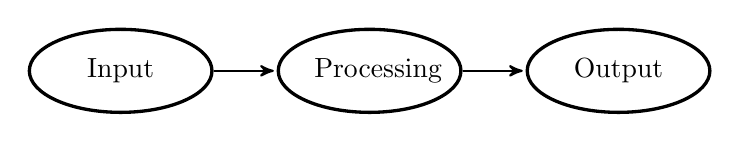
\begin{tikzpicture}
      [>=stealth',
        element/.style={
          ellipse,
          draw=black, very thick,
          text width=4em,
          minimum height=3em,
          text centered,
          on chain},
        line/.style={draw, thick, <-},
        every join/.style={->, thick,shorten >=1pt},
        node distance=.8cm,
        start chain=going right,]
      \node[element, join] (input) {Input};
      \node[element, join] (processing) {Processing};
      \node[element, join] (output) {Output};
    \end{tikzpicture}
    }

      {\small
        \bibliographystyle{plain}
        \bibliography{slides}{}
      }

    \end{column}
    \begin{column}{.5\textwidth}
    \resizebox{\textwidth}{!}{
    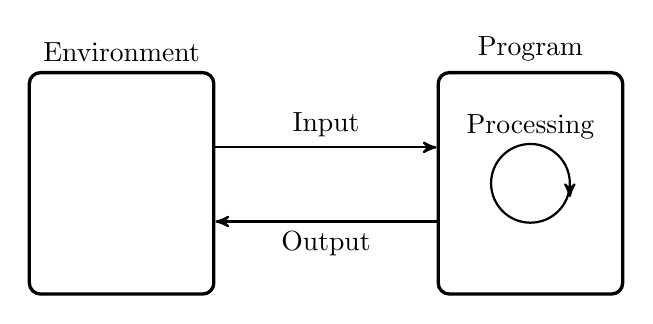
\begin{tikzpicture}
      [>=stealth',
        line/.style={draw, thick, ->},
        entity/.style={
          rectangle,
          rounded corners,
          draw=black, very thick,
          text centered,
          text width=6em,
          minimum height=8em,
}]
      \node[entity, label={Environment}] (environment) {};
      \node[entity, right=4cm, label={Program}] (program) at (environment) {};
      \draw[line] ($(environment.south east)!0.66!(environment.north east)$) -- ($(program.south west)!0.66!(program.north west)$) node [midway, above] {Input};
      \draw[line] ($(program.south west)!0.33!(program.north west)$) -- ($(environment.south east)!0.33!(environment.north east)$) node [midway, below] {Output};

      \draw[line,
        decoration={markings, mark=at position 0.0 with {\arrow{<}}},
        postaction={decorate}
      ]
      (program) circle (0.5) node [label={[label distance=.3cm]90:Processing}] {};
    \end{tikzpicture}
    }
    \end{column}
  \end{columns}

  %%\rule{\textwidth}{0.4pt}

  \begin{columns}
    \begin{column}{.7\textwidth}
      \begin{center}
      {\Large Contributions}
      \end{center}

      \begin{itemize}
        \item Formal Model - Reactive Components
        \item Programming Language - \rcgo{}
        \item Platform
        \item Scheduler Evaluation
      \end{itemize}
    \end{column}
    \begin{column}{.3\textwidth}

      \begin{center}
        
\includegraphics[width=1.25cm]{smartphone.jpg}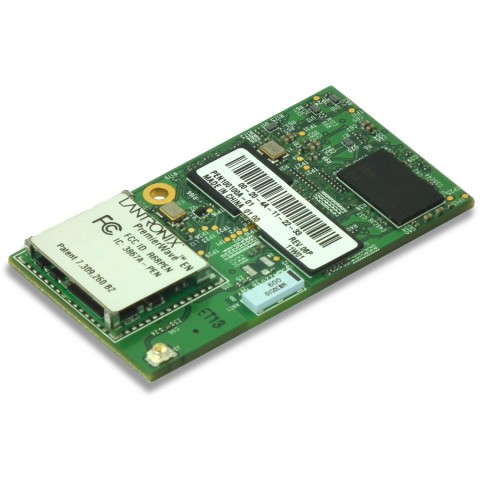
\includegraphics[width=1.25cm]{embedded.jpg}

        \vspace*{12pt}

        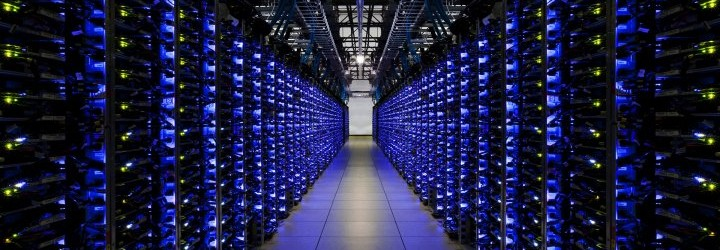
\includegraphics[height=1cm]{servers.jpg}
      \end{center}

    \end{column}
  \end{columns}

\end{frame}

\begin{frame}{Fundamental Characteristics of Reactive Systems}

  \begin{columns}
    \begin{column}{.5\textwidth}
  \centering

  \resizebox{!}{.8\textheight}{
    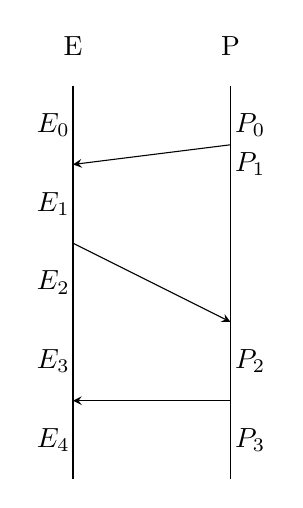
\begin{tikzpicture}
      [
        arrowstyle/.style={draw, -stealth}
      ]

      \node (a) at (0,.5) {E};
      \draw (0,0) -- (0,-5);
      \node at (-.25,-.5) {$E_0$};
      \node at (-.25,-1.5) {$E_1$};
      \node at (-.25,-2.5) {$E_2$};
      \node at (-.25,-3.5) {$E_3$};
      \node at (-.25,-4.5) {$E_4$};

      \node (b) at (2,.5) {P};
      \draw (2,0) -- (2,-5);
      \node at (2.25,-.5) {$P_0$};
      \node at (2.25,-1) {$P_1$};
      \node at (2.25,-3.5) {$P_2$};
      \node at (2.25,-4.5) {$P_3$};

      \draw[arrowstyle] (2,-.75) -- (0,-1);
      \draw[arrowstyle] (0,-2) -- (2,-3);
      \draw[arrowstyle] (2,-4) -- (0,-4);

    \end{tikzpicture}
  }
    \end{column}
    \begin{column}{.5\textwidth}

      {
        \begin{block}{Time and State}
          Reason about the \emph{state} of the program relative to the \emph{state} of the environment.
        \end{block}

        \begin{block}{Concurrency}
          A program and its environment may act at the same time.
        \end{block}

        \begin{block}{Synchronous Systems}
          Program and environment share a common clock.
        \end{block}

        \begin{block}{Asynchronous Systems}
          Program and environment do not share a common clock (this work).
        \end{block}
      }

  %% \begin{block}{State (and Time)}
  %%   To simplify reasoning, we assume reactive programs have state variables manipulated by assignment statements.
  %% \end{block}

    \end{column}
  \end{columns}
  %% \begin{block}{Examples}
  %%   Operating Systems, Clients/Servers, Databases, Embedded Systems, Smart Phone Apps, Web Applications, etc.
  %% \end{block}

\end{frame}

\begin{frame}{Trends}

  \begin{block}{Enabling Technologies}

  \begin{columns}
    \begin{column}{.5\textwidth}
      \begin{itemize}
      \item \emph{Form Factors} \\ new domains
      \item \emph{(Wireless) Networking} \\ new frontiers
      %% \item \emph{IaaS/PaaS/SaaS} \\ rapid deployment
      %% \item \emph{Services and Microservices} \\ integration over implementation
      \end{itemize}
    \end{column}
    \begin{column}{.5\textwidth}
      \centering

      
\includegraphics[width=1.25cm]{smartphone.jpg}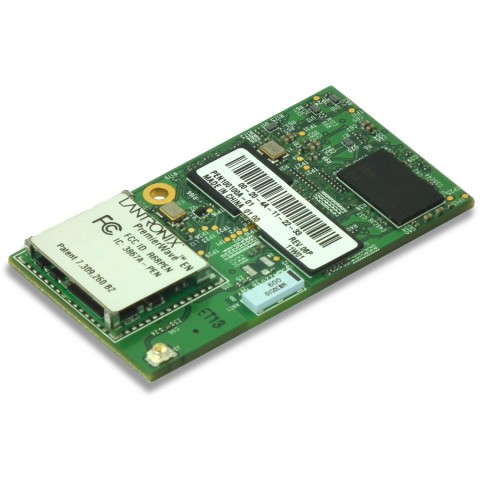
\includegraphics[width=1.25cm]{embedded.jpg}

      \vspace*{12pt}

      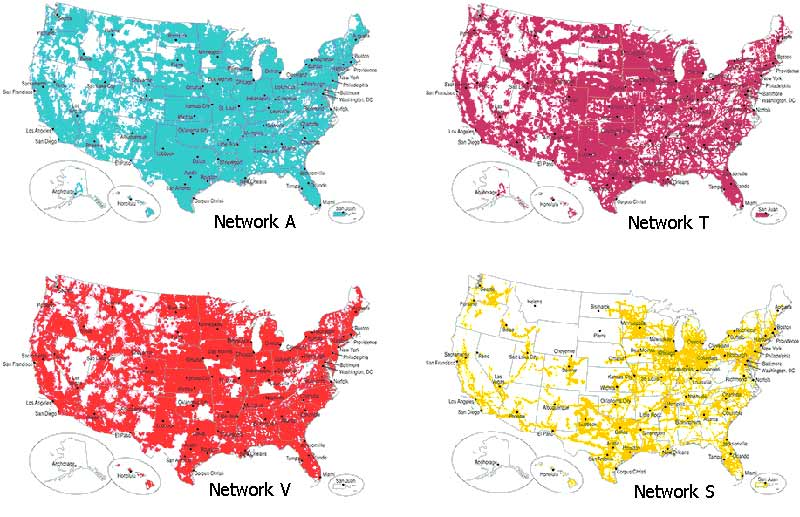
\includegraphics[height=1.25cm]{cellmap.jpg}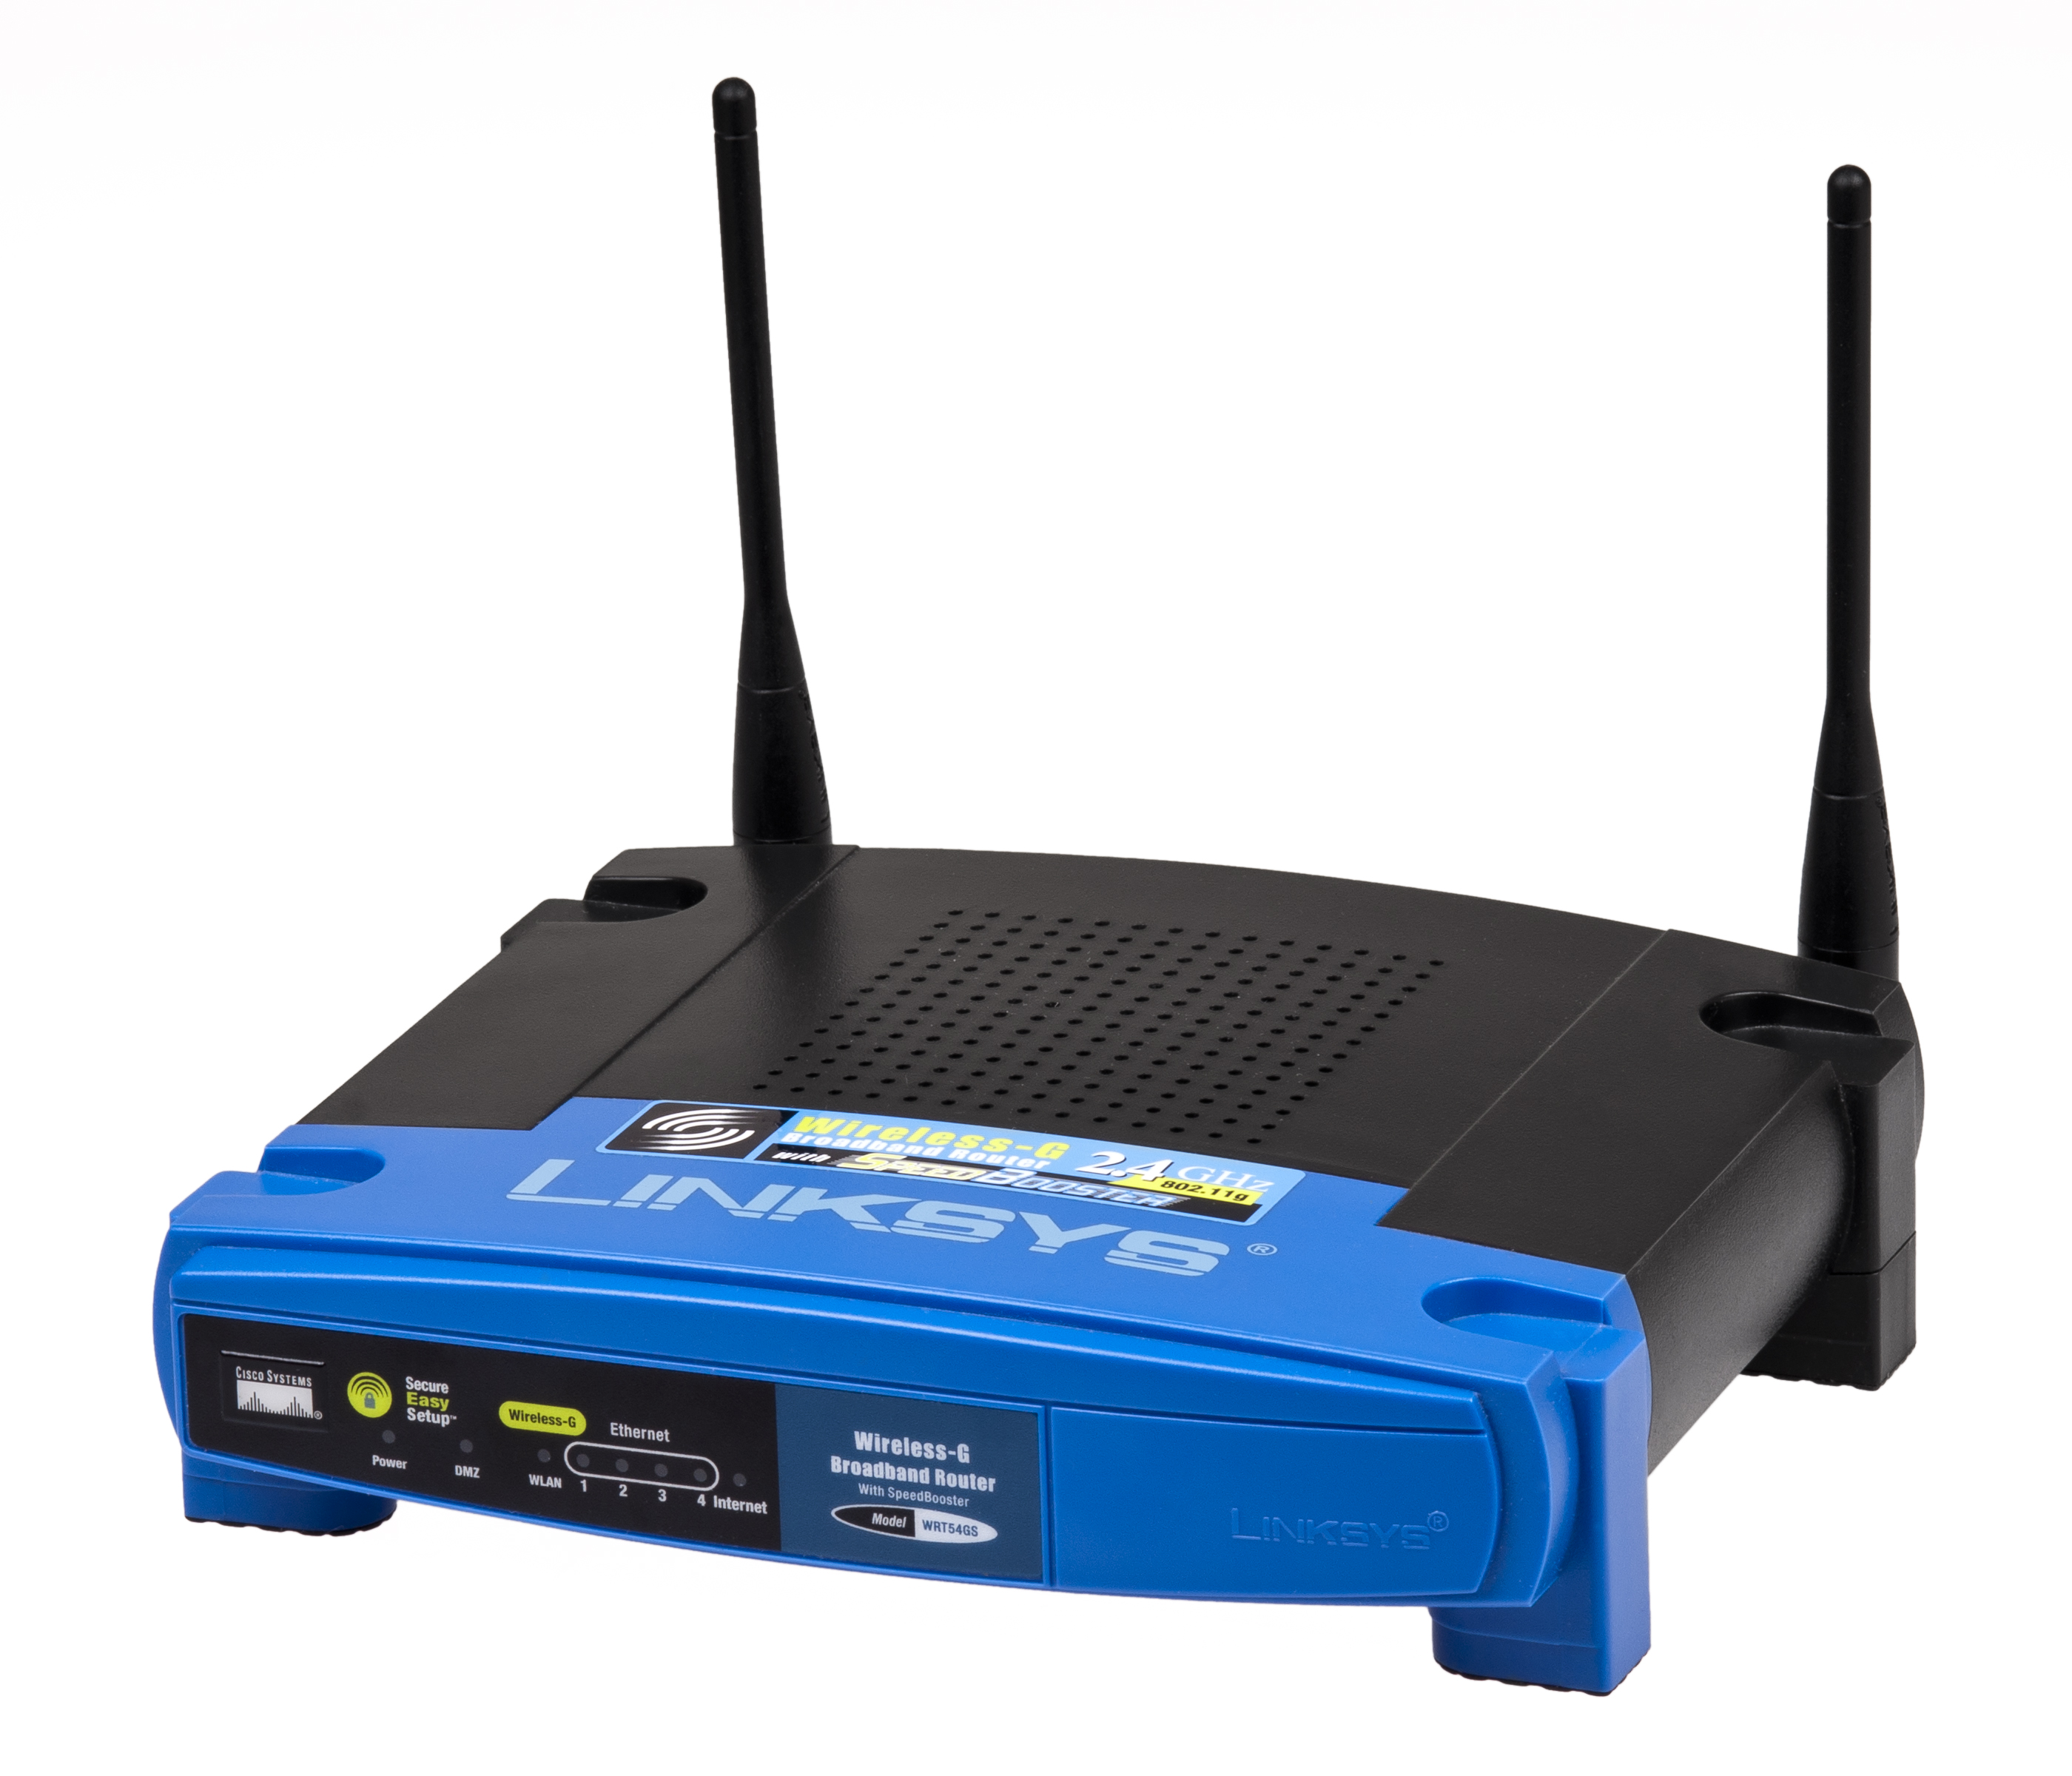
\includegraphics[height=1.25cm]{wirelessrouter.jpg}

      %% \vspace*{12pt}

      %% 
\includegraphics[height=1.25cm]{cloud.png}

      %% \vspace*{12pt}

      %% 
\includegraphics[height=1.25cm]{kafka_logo.png}
\includegraphics[height=1.25cm]{elasticsearch.png}

    \end{column}
  \end{columns}
  \end{block}

  \begin{block}{Consequences}

  \begin{columns}
    \begin{column}{.5\textwidth}
      \begin{itemize}
      \item \emph{Scale} \\ large systems require different techniques

      \item \emph{Complexity} \\ systems of systems of \ldots

      %\item \emph{Heterogeneity} \\ systems incorporate software/services from a variety of sources
      \end{itemize}

    \end{column}
    \begin{column}{.5\textwidth}
      \centering

      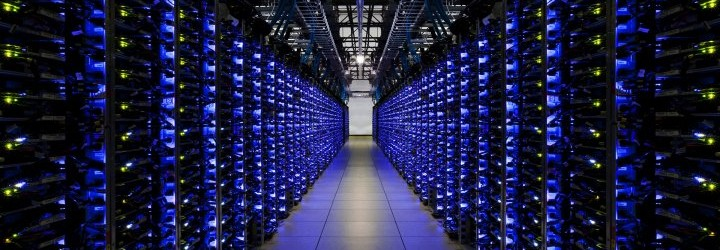
\includegraphics[height=1cm]{servers.jpg}

      \vspace*{12pt}

      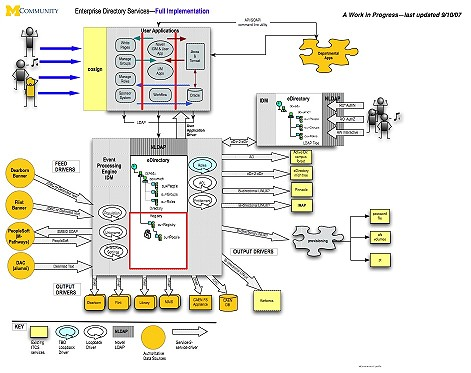
\includegraphics[height=1.5cm]{system.jpg}

      %% \vspace*{12pt}

      %% 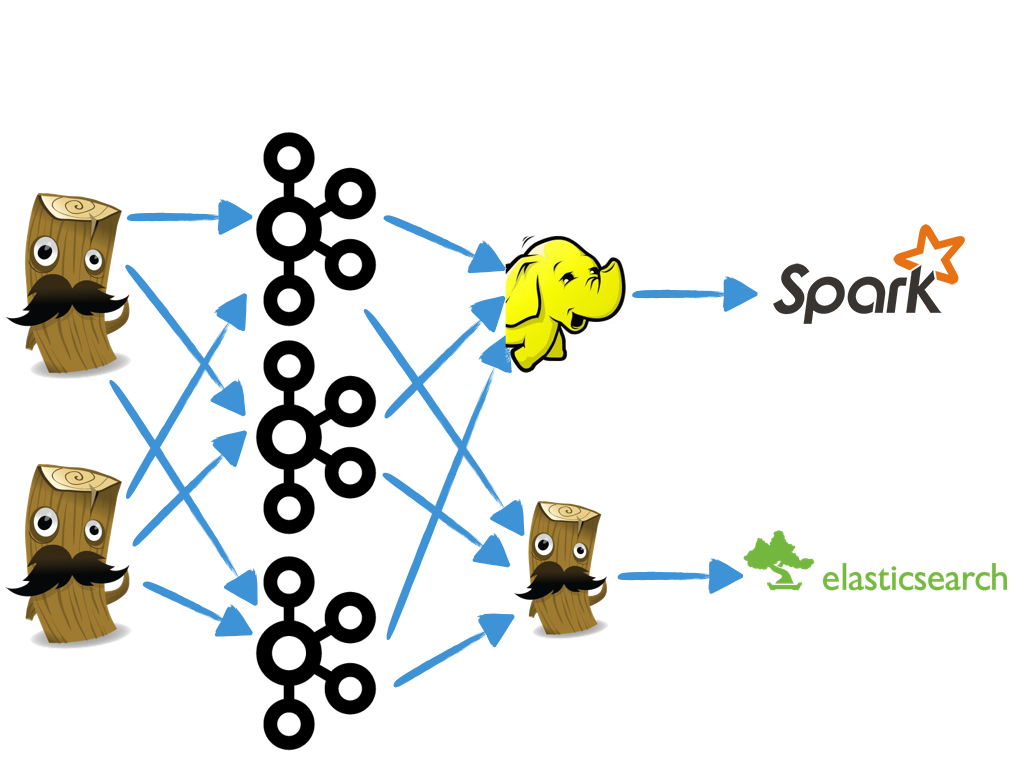
\includegraphics[height=1.5cm]{integration.png}
    \end{column}
  \end{columns}

  \end{block}
\end{frame}

\begin{frame}{The Goal}

  \Large

  An abstraction that makes reactive programs easy to
  \begin{itemize}
  \item design
  \item implement
  \item test
  \item debug
  \item reuse
  \end{itemize}
  without sacrificing performance.

\end{frame}

\begin{frame}{Limitations of the State of the Art:  Threads and Events}
  \begin{columns}
    \begin{column}{.6\textwidth}

      \resizebox{\textwidth}{!}{
        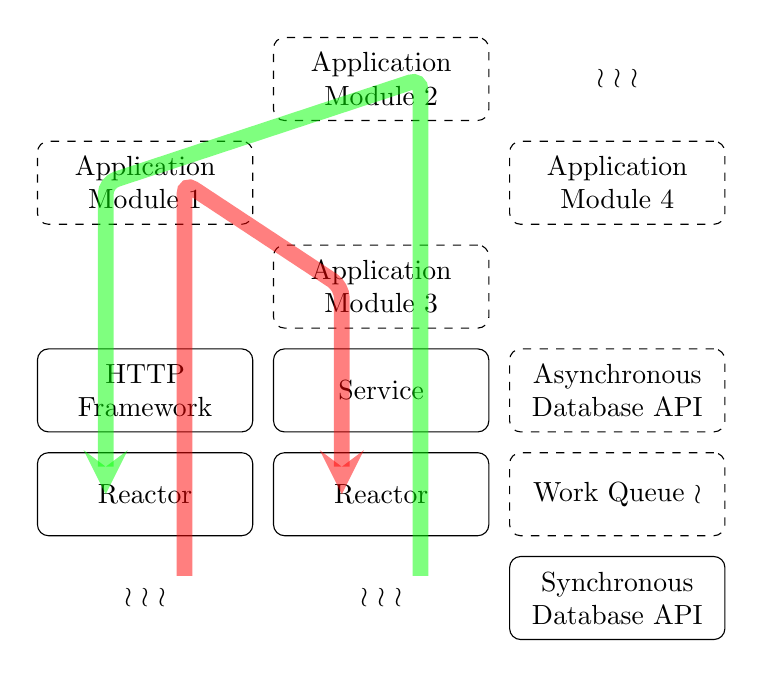
\begin{tikzpicture}
          [ ampersand replacement=\&,
            element/.style={
              rectangle,
              draw,
              rounded corners,
              text width=2.5cm,
              minimum height=3em,
              text centered},
            line/.style={
              draw,
              thick,
              ->,
              >=stealth,
              line width=2mm,
              opacity=.5,
              rounded corners,
            },
          ]

          \matrix [row sep=.25cm, column sep=.25cm] {
            \&
            \node (apm2) [element, dashed] {Application Module 2}; \&
            \node {$\wr$ $\wr$ $\wr$}; \\

            \node (apm1) [element, dashed] {Application Module 1}; \&
            \&
            \node [element, dashed] {Application Module 4}; \\

            \&
            \node (apm3) [element, dashed] {Application Module 3}; \&
            \\

            \node (http) [element] {HTTP Framework}; \&
            \node (service) [element] {Service}; \&
            \node [element, dashed] {Asynchronous Database API}; \\

            \node (reactor1) [element] {Reactor}; \&
            \node (reactor2) [element] {Reactor}; \&
            \node [element, dashed] {Work Queue $\wr$}; \\

            \node (thread1) {$\wr$ $\wr$ $\wr$}; \&
            \node (thread2) {$\wr$ $\wr$ $\wr$}; \&
            \node [element] {Synchronous Database API}; \\
          };

          \draw[line,red] ($(thread1.north) + (.5,0)$) -- ($(reactor1.center) + (.5,0)$) -- ($(http.center) + (.5,0)$) -- ($(apm1.center) + (.5,0)$) -- ($(apm3.center) - (.5,0)$) -- ($(service.center) - (.5,0)$) -- ($(reactor2.center) - (.5,0)$);

          \draw[line,green] ($(thread2.north) + (.5,0)$) -- ($(service.center) + (.5,0)$) -- ($(apm3.center) + (.5,0)$) -- ($(apm2.center) + (.5,0)$) -- ($(apm1.center) + (-.5,0)$) -- ($(http.center) - (.5,0)$) -- ($(reactor1.center) - (.5,0)$);

        \end{tikzpicture}
      }
    \end{column}

    \begin{column}{.4\textwidth}
      \begin{block}{Hazards}
        \begin{itemize}
          \item deadlock
          \item livelock
          \item memory corruption
        \end{itemize}
      \end{block}
      \begin{block}{Brittle unless developers}
        \begin{itemize}
        \item identify and protect shared state
        \item understand call graph
        \end{itemize}
      \end{block}

    \end{column}
  \end{columns}

\end{frame}

\begin{frame}{Challenges}

  \begin{block}{Reduce Accidental Complexity}
    \begin{itemize}
    \item implicit atomicity
    \item eliminate uncoordinated access to shared state
    \end{itemize}
  \end{block}

  \begin{block}{Achieve Principled Composition}
    \begin{enumerate}
    \item Define units and means of composition
    \item ``Well-formed-ness''
    \item Recursive Encapsulation - units may contain other units (hierarchical reasoning)
    \item Interfaces - reason about interface instead of implementation
    \item Compositionality - reason about whole from parts
    \item Substitutional Equivalence - substitute definition for use
    \end{enumerate}
  \end{block}
\end{frame}

%% \begin{frame}{Compositionality and Substitutional Equivalence}

%%   \begin{columns}
%%     \begin{column}[T]{.45\textwidth}
%%       \begin{block}{Compositionality}
%%         $f(x) \mod 2 = 1$ (odd)

%%         $g(x) \mod 2 = 1$ (odd)

%%         $h(x) = f(x) + g(x)$

%%         $h(x) \mod 2 = ?$
%%       \end{block}
%%     \end{column}
%%     \begin{column}[T]{.45\textwidth}
%%       \begin{block}{Substitutional Equivalence}
%%         $f(x) = 2x$

%%         $g(x) = x+1$

%%         $h(x) = f(g(x)) = 2(x+1)$

%%         $h(x) = 2x + 2$
%%       \end{block}
%%     \end{column}
%%   \end{columns}

%%   \vspace*{24pt}

%%   \begin{center}
%%     \LARGE
%%     Straightforward for simple algebras.  How can we achieve this in reactive systems?
%%   \end{center}

%% \end{frame}

\begin{frame}{Related Work}

  Abstract Models for Analysis
  \begin{itemize}
  \item e.g., Calculus of Communicating Systems, Algebra of Communicating Processes
  \item Not practical for design and implementation
  \end{itemize}

  Processes-Oriented Models
  \begin{itemize}
  \item e.g., Cooperating Sequential Processes, Communicating Sequential Processes, Kahn Process Networks
  \item Difficult to rewrite $N$ processes as one process
  \end{itemize}

  Asynchronous Message Passing
  \begin{itemize}
  \item e.g., Actor Model
  \item Weak guarantees limit compositional design and reasoning
  \end{itemize}
\end{frame}

\begin{frame}{Related Work}
  UNITY
  \begin{itemize}
  \item State variables, parallel assignment statements, non-deterministic selection and execution
  \item Lack of encapsulation/interface precludes compositionality
  \end{itemize}

  I/O Automata
  \begin{itemize}
  \item State variables, input/output/internal actions, pre/post conditions, signatures (interfaces)
  \item Named-based composition limited in depth
  \end{itemize}

\end{frame}

\begin{frame}[fragile]{Approach and Contributions}
  \centering
  \begin{tabular}{|C{.4\textwidth}|C{.4\textwidth}|}
    \hline
     \emph{Reactive Components} \newline \emph{Formal Model} & \rcgo{} \newline Programming Language \\

     \resizebox{.25\textwidth}{!}{%
       \chapter{Reactive Component Model}
\label{model}

In this chapter, we present a new model for composing and decomposing reactive programs via \emph{reactive components}.
The model is biased toward practical software development even as it enforces properties based in formal methods.
Consequently, the model favors utility, practicality, flexibility, and ease of implementation.
Unlike UNITY in which composition is not property-preserving, the composition of reactive components is property-preserving which facilitates hierarchical and modular reasoning.
Unlike I/O Automata in which transitions have limited depth, a transition among reactive components may access and cascade to an arbitrary number of other components, which permits decomposition to an arbitrary depth and degree.

%% \paragraph{Formal models and software engineering.}
%% I claim that most of the software that is ``put into production'' will never be proved formally correct.
%% This is a function of economics since modeling and constructing proofs is a labor-intensive process that can only be justified for safety or mission critical software.
%% However, I would argue that the development and application of formal models are critical to software engineering.
%% To illustrate, consider \emph{structured programming}~\cite{dahl1972structured}.
%% Structured programming assumes an abstract machine that executes programs that are restricted to a small set of well-defined control structures and assignment statements.
%% A program written in this form can be reasoned about directly from the text by formulating a Hoare-triple for each statement.
%% Structured programming opened the door for \emph{structured programming languages} which are also based on well-defined control structures and evaluation semantics.
%% Thus, while very few programmers will prove their structured programs correct, all of them informally use structured programming when they are fixing a bug revealed by a unit test or analyzing a core dump in a debugger.
%% Structured programming languages reduced the accidental complexity associated with writing the same program in assembly language.

%% The realm of reactive programs is waiting for a similar reduction in accidental complexity.
%% Taking a hint from structured programming, I believe two things are required.
%% First, we must write reactive programs against an easy-to-reason-about abstract machine instead of low-level interfaces like atomic instructions and thread libraries.
%% Second, we must restrict the form of reactive programs so that they can be reasoned about from the text.
%% I hope the proposed model of reactive systems is a step toward toward this goal.

\section{Features of the Model}

%% left active pull port
%% x, y, width, height, label
\def\lapull[#1,#2,#3,#4,#5,#6]#7{
  \draw [fill=lightgray] (#1,#2) -- ++(${#4*.5}*(-1,0) + {#4*.5}*(0,-1)$) -- ++($#3*(1,0)$) -- ++($#4*(0,1)$) -- ++($#3*(-1,0)$) -- cycle;
  \node (#5) at (#1,#2) {};
  \node (#6) at ($(#1,#2) + {#3 - .5 * #4}*(1,0)$) {};
  \node [right, align=left] at (#1,#2) {#7};
}

%% left active push port
%% x, y, width, height, label
\def\lapush[#1,#2,#3,#4,#5,#6]#7{
  \draw [fill=white] ($(#1,#2) + {#4*.5}*(-1,0)$) -- ++(${#4*.5}*(1,0) + {#4*.5}*(0,-1)$) -- ++($#3*(1,0)$) -- ++($#4*(0,1)$) -- ++($#3*(-1,0)$) -- cycle;
  \node (#5) at ($(#1,#2) - .5*#4*(1,0)$) {};
  \node (#6) at ($(#1,#2) + {#3}*(1,0)$) {};
  \node [right, align=left] at (#1,#2) {#7};
}

%% left passive pull port
%% x, y, width, height, label
\def\lppull[#1,#2,#3,#4,#5,#6]#7{
  \draw [fill=lightgray] ($(#1,#2) + {#4*.5}*(-1,0)$) -- ++(${#4*.5}*(1,0) + {#4*.5}*(0,-1)$) -- ++($#3*(1,0)$) -- ++($#4*(0,1)$) -- ++($#3*(-1,0)$) -- cycle;
  \node (#5) at ($(#1,#2) - .5*#4*(1,0)$) {};
  \node (#6) at ($(#1,#2) + {#3}*(1,0)$) {};
  \node [right, align=left] at (#1,#2) {#7};
}

%% left passive push port
%% x, y, width, height, label
\def\lppush[#1,#2,#3,#4,#5,#6]#7{
  \draw [fill=white] (#1,#2) -- ++(${#4*.5}*(-1,0) + {#4*.5}*(0,-1)$) -- ++($#3*(1,0)$) -- ++($#4*(0,1)$) -- ++($#3*(-1,0)$) -- cycle;
  \node (#5) at (#1,#2) {};
  \node (#6) at ($(#1,#2) + {#3 - .5*#4}*(1,0)$) {};
  \node [right, align=left] at (#1,#2) {#7};
}

%% right passive pull port
%% x, y, width, height, label
\def\rppull[#1,#2,#3,#4,#5,#6]#7{
  \draw [fill=lightgray] ($(#1,#2) + {#4*.5}*(1,0)$) -- ++(${#4*.5}*(-1,0) + {#4*.5}*(0,-1)$) -- ++($#3*(-1,0)$) -- ++($#4*(0,1)$) -- ++($#3*(1,0)$) -- cycle;
  \node (#5) at ($(#1,#2) + {#4*.5}*(1,0)$) {};
  \node (#6) at ($(#1,#2) + {#3}*(-1,0)$) {};
  \node [left] at (#1,#2) {#7};
}

%% right active push port
%% x, y, width, height, label
\def\rapush[#1,#2,#3,#4,#5,#6]#7{
  \draw [fill=white] ($(#1,#2) + {#4*.5}*(1,0)$) -- ++(${#4*.5}*(-1,0) + {#4*.5}*(0,-1)$) -- ++($#3*(-1,0)$) -- ++($#4*(0,1)$) -- ++($#3*(1,0)$) -- cycle;
  \node (#5) at ($(#1,#2) + {#4*.5}*(1,0)$) {};
  \node (#6) at ($(#1,#2) + {#3}*(-1,0)$) {};
  \node [left] at (#1,#2) {#7};
}

%% right passive push port
%% x, y, width, height, label
\def\rppush[#1,#2,#3,#4,#5,#6]#7{
  \draw [fill=white] (#1,#2) -- ++(${#4*.5}*(1,0) + {#4*.5}*(0,-1)$) -- ++($#3*(-1,0)$) -- ++($#4*(0,1)$) -- ++($#3*(1,0)$) -- cycle;
  \node (#5) at (#1,#2) {};
  \node (#6) at ($(#1,#2) + {#3 - .5*#4}*(-1,0)$) {};
  \node [left] at (#1,#2) {#7};
}

%% right active pull port
%% x, y, width, height, label
\def\rapull[#1,#2,#3,#4,#5,#6]#7{
  \draw [fill=lightgray] (#1,#2) -- ++(${#4*.5}*(1,0) + {#4*.5}*(0,-1)$) -- ++($#3*(-1,0)$) -- ++($#4*(0,1)$) -- ++($#3*(1,0)$) -- cycle;
  \node (#5) at (#1,#2) {};
  \node (#6) at ($(#1,#2) + {#3 - .5*#4}*(-1,0)$) {};
  \node [left] at (#1,#2) {#7};
}

\begin{figure}[H]
\centering
\resizebox{\textwidth}{!}{%
\begingroup
\fontsize{10pt}{12pt}\selectfont
\begin{tikzpicture}
[
arrowstyle/.style={
  decoration={markings,mark=at position 1 with {\arrow[scale=2,]{stealth}}},
  postaction={decorate},
  shorten >=0.4pt
}
]

%% component boundary
\draw (0,0) rectangle (10,8.25);
%% active pull ports
\lapull[0,1.5,1,.5,apullex1,apullin1]{}
\node[align=center] at (-1,1.5) {active\\pull port};
\lapull[0,.5,1,.5,apullex2,apullin2]{}
%% passive pull ports
\rppull[10,1.5,1,.5,ppullex1,ppullin1]{}
\node[align=center] at (11,1.5) {passive\\pull port};
\rppull[10,.5,1,.5,ppullex2,ppullin2]{}
\draw[thick] (apullin2.center) -- (ppullin2.center);
%% actions and rections
\node[draw, diamond, minimum height=15, minimum width=20] (pre) at (2.5,3) {};
\node at (2.5,2.5) {precondition};
\node[draw, minimum height=15, minimum width=50, rounded corners=5] (trans1) at (5,3) {};
\draw[dashed] (3.5,3) ellipse (3 and 1);
\node at (3.5,3.5) {\textbf{\emph{action}}};
\node[draw, minimum height=15, minimum width=50, rounded corners=5] (trans2) at (5,5) {};
\node at (5,4.5) {transition};
\draw[thick,arrowstyle] (pre) -- (trans1);
\draw[thick] (apullin1.center) -| (trans1) node[pos=.5,right] {\textbf{call}};
%% active push ports
\rapush[10,3,1,.5,apushex1,apushin1]{}
\rapush[10,4,1,.5,apushex2,apushin2]{}
\rapush[10,5,1,.5,apushex3,apushin3]{}
\node[align=center] at (11.1,5) {active\\push port};
\draw[thick,dashed,arrowstyle] (trans1) -- (apushin1.center);
\draw[thick,dashed,arrowstyle] (trans1) -- (apushin2.center);
\node at(7.5,4) {\textbf{activate}};
\draw[thick,dashed,arrowstyle] (trans2) -- (apushin2.center);
\draw[thick,dashed,arrowstyle] (trans2) -- (apushin3.center);
%% passive push ports
\lppush[0,5,1,.5,ppushex1,ppushin1]{}
\draw[thick,arrowstyle] (ppushin1.center) -- (trans2);
\node[align=center] at (-1.1,5) {passive\\push port};
\draw[dashed] (2,5) ellipse (5 and 1);
\node at (2,5.5) {\textbf{\emph{reaction}}};
\node[draw, cylinder, shape border rotate=90, minimum height=40, minimum width=40] (sv1) at (5,7.25) {};
\node[align=center] at (5,6.25) {state variables};
\end{tikzpicture}
\endgroup
}%
\caption{Features of a reactive component\label{reactive_component}}
\end{figure}

Figure~\ref{reactive_component} shows the major features of a reactive component.
As in other state-based formal models like UNITY~\cite{chandy1989parallel} and I/O Automata~\cite{nancy1996distributed}, the core of a reactive component in this model is a set of \emph{state variables} and a set of atomic \emph{transitions} that manipulate those state variables.
When reasoning about a system, behavior is expressed as propositions over the state variables where the propositions are derived from the transitions.

%% The contribution that this work makes to existing state-based formal models of reactive systems is a combination of interface elements and composition semantics that allow reactive programs to be composed in a principled way.

The reactive component model defines interface elements and composition semantics that allow reactive programs to be composed in a principled way.
For example, an \emph{active push port} allows a transition in one component to be linked to a transition in another component such that the resulting combined transition is atomic.
Active push ports allow reactive components to publicize their behavior.
An active push port may be \emph{bound} to and conditionally \emph{activate} zero or more \emph{passive push ports}.
A passive push port names the corresponding transition that will be executed when the passive push port is activated.
This combination of passive push port and transition is called a \emph{reaction} because it reacts to a transition in another component.

The atomic linkage of a transition in one component to a transition in another component through the push port mechanism allows the properties of each component to be related to one another and more complex systems to be constructed by composing simpler systems.
Transitions that are not executed via a passive push port are executed by the scheduler.
A transition of this kind may be governed by a Boolean expression called a \emph{precondition}.
The combination of a precondition and transition is called an \emph{action} because it is a voluntary transition under the control of the containing component.

An \emph{active pull port} represents an immutable external data dependency.
The component may \emph{call} an active pull port to yield a value required in a transition.
Active pull ports must be bound to a \emph{passive pull port} which resembles a function returning a value, e.g., a getter or a predicate.
Where push ports allow components to publicize their behavior, pull ports allow components to safely publicize their internal state for use by other components.

Composition in the reactive component model has two main features.
The first is recursive encapsulation where a state variable in one component may represent an instance of another reactive component.
The second is the ability to bind push ports and pull ports through an \emph{explicit} set of \emph{bindings}.
The decision to use an explicit set of bindings (as opposed to implicit named-based matching) is more in keeping with the goals and techniques of practical software development, since it facilitates the use of software developed under different naming conventions, i.e., third-party software.
A third minor feature called \emph{exporting} is the ability of an encapsulating component to adopt interface elements of its sub-components without defining complimentary ports and transitions that do nothing but forward an activation or call.
The ability to publicize behavior and state and the ability to assemble well-defined behavior from existing behaviors in a straight-forward and flexible way are thus defining characteristics of the reactive component model.

\begin{figure}
\centering
\resizebox{\textwidth}{!}{%
\begingroup
\fontsize{10pt}{12pt}\selectfont
\begin{tikzpicture}
\draw (0,6.5) rectangle (5,10);
\node[below] at (2.5,10) {Web Server};
\rapull[5,9,3.4,.5,ex1a,ignore]{verify(HttpHeader)};
\rapush[5,8,3.6,.5,ex2a,ignore]{request(HttpRequest)};
\rppush[5,7,4.2,.5,ex3a,ignore]{respond(HttpResponse)};

\draw(6,2.5) rectangle (11,10);
\node[below] at (8.5,10) {Application Logic};
\lppull[6,9,3.4,.5,ex1b,ignore]{verify(HttpHeader)};
\lppush[6,8,3.8,.5,ex2b,ignore]{request(HttpRequest)};
\lapush[6,7,3.9,.5,ex3b,ignore]{respond(HttpResponse)};

\rapush[11,6,3.5,.5,ex4a,ignore]{request(DBRequest)};
\rppush[11,5,4.1,.5,ex5a,ignore]{respond(DBResponse)};

\rapush[11,3,2.4,.5,ex6a,ignore]{log(Message)};

\draw (12,4.5) rectangle (17,7);
\node[below] at (14.5,7) {Database};
\lppush[12,6,3.7,.5,ex4b,ignore]{request(DBRequest)};
\lapush[12,5,3.8,.5,ex5b,ignore]{respond(DBResponse)};

\draw (12,2.5) rectangle (17,4);
\node[below] at (14.5,4) {Logging Service};
\lppush[12,3,2.5,.5,ex6b,ignore]{log(Message)};

\draw (ex1a.center) -- (ex1b.center);
\draw (ex2a.center) -- (ex2b.center);
\draw (ex3a.center) -- (ex3b.center);
\draw (ex4a.center) -- (ex4b.center);
\draw (ex5a.center) -- (ex5b.center);
\draw (ex6a.center) -- (ex6b.center);

\end{tikzpicture}
\endgroup
}%
\caption{Diagram of a web application built using reactive components\label{web_server}}
\end{figure}

To demonstrate the utility of component interfaces and explicit support for property-preserving composition, we now present an illustrative design for a web application using reactive components, as is shown in Figure~\ref{web_server}.
The web application consists of five reactive components.
The first is an unnamed top-level component representing the complete application.
This component has four sub-components representing a web server, the application logic, a database, and a logging service.
The ports of the application logic component have been bound to the corresponding ports in the web server, database, and logging service components.
The interface of a component, which consists of its ports, provides insight into the behavior of the component.
For example, based on the interface of the web server component we may expect it to 1)~verify incoming HTTP requests\footnote{A production web server may verify that the requested HTTP method can be applied to the given URI, that content length limits are respected, that content types are supported, etc.}, 2)~pass on valid HTTP requests to the application, and 3)~accept HTTP responses from the application.

Figure~\ref{web_server} also demonstrates how reactive programs can be constructed by composing reactive components, so that a developer may focus on the application logic and use existing components for the web server, database, and logging service.
Furthermore, one can imagine developing three stateless components surrounding the application logic that do nothing but translate messages between application specific message types and the generic types required by the web server, database, and logging service.
The application logic, then, is completely isolated from the surrounding libraries and may be tested by providing mock components for the web server, database, and logging service.
The application logic itself has a well-defined interface and could be reused, say, by implementing a graphical front-end to drive the application instead of a web service.

\subsection{State Variables}
Part of the internal core of a reactive component is a set of state variables, which are the subject of the propositions that demonstrate the behavior of the system.
The state variables are manipulated by the assignment statements that constitute the transitions.
As in other formal models, the types of the state variables may be selected to make writing proofs easier.
%% That is, the state variables have mathematically friendly types like integers, sets, and lists.
However, implementations of the reactive component model must provide a concrete type system that allows the state variables to be realized on a given machine.
For example, the \rcgo{} language for reactive components presented in Chapter~\ref{language} of this dissertation uses the type system of Go to define the types of state variables.
The type of a state variable also may be a reactive component type, which facilitates recursive encapsulation.
For modeling purposes, state variables typically have \emph{value semantics} to avoid reasoning about references and aliasing.
However, and as a practical concession, we will introduce pointers for building arbitrary linked data structures (since we advocate an imperative state-based implementation) and discuss issues raised by introducing pointers into the reactive component model in Chapter~\ref{language}.

\subsection{Atomic State Transitions}
The rest of the internal core of a reactive component is a set of atomic state transitions that manipulate the state variables.
A precise definition of the atomicity of state transitions will be deferred to the subsequent sections on composition (Section~\ref{composition}) and execution (Section~\ref{execution}).
State variables and state transitions are private, meaning that transitions can only refer to the state variables of the associated reactive component and a transition in one reactive component can only be linked to a transition in another component through the composition mechanisms.
Thus, all initialization and updates to state variables can be determined by examining the transitions of the corresponding component.
The encapsulation of state variables contribute to composition being \emph{compositional}.
All properties established from the transitions of a component will continue to hold as the component participates in composition since the set of transitions that affect the state variables is fixed.
State transitions must be deterministic meaning that the next value of every state variable is uniquely and well defined.
State transitions defined by a sequence of simple assignments are implicitly deterministic.
However, special care must be take to ensure that state transitions are deterministic when described using parallel assignment statements as the same variable may appear on the left-hand-side and be assigned two different values~\cite{chandy1989parallel}.
As described in Sections~\ref{composition} and \ref{execution}, composition links transitions using parallel assignment which creates an opportunity for non-deterministic state transitions.
The problem of non-deterministic state transitions arising from composition is explored in Section~\ref{propcomp}.

The reactive component model presented in this chapter does not prescribe a specific language for encoding state transitions.
The language used depends on the goals and tastes of the one developing or analyzing the model.
For example, expressing transitions using the programming language of UNITY~\cite{chandy1989parallel} may allow the modeler to extract proofs from the text, a major goal of UNITY.
The approach used by I/O Automata~\cite{nancy1996distributed} is to specify the condition established by each transition.
As with state variables, we present a language that uses the statements and expressions of the Go programming language to encode state transitions in Chapter~\ref{language}.
This furthers our goal of making reactive components approachable by a general software engineering audience.
%% from Dr. Gill
%% which aims to allow models to be incorporated directly into standard software environments.
%% This isn't accurate.  Compatibility with existing software is not the goal nor should it be a goal as existing software is based on threads which cannot reasonably be integrated with reactive components.

\subsection{Actions, Reactions, Push Ports, Bindings, and Composition}
\label{composition}
A state transition is either part of an action or a reaction.
An \emph{action} is a state transition whose execution is under the control of the component to which it belongs.
The action is guarded by a \emph{precondition} that is guaranteed to be true the instant before the action is executed.
The precondition is a Boolean expression that determines if the action is \emph{enabled} or \emph{disabled}.
If the precondition is absent, it is assumed to be true.

A \emph{reaction} is a state transition whose execution is under the control of another action or reaction.
Thus, we require a mechanism for linking a reaction to an action or another reaction.
To do this, we introduce the notion of a \emph{push port}.
A push port is a typed interaction point consisting of an active side that conditionally \emph{activates} the port and provides arguments to the port, and a passive side that \emph{reacts} to the port and may access the arguments provided by the active side.
A reaction, therefore, is the combination of a passive push port and a state transition.

A \emph{binding} is a declaration that associates an active push port in one component with a reaction in another component.
The transition associated with the reaction is executed atomically with the transition that activates the active push port.
Composition in the reactive component model is achieved by declaring sub-components (recursive encapsulation) and linking transitions via binding.

\subsection{Transactions}

A \emph{transaction} is a compound and concrete state transition formed by expanding the activations in an instance/action pair, subject to the bindings in a system.
The instance and action that define a transaction are called the \emph{root} of the transaction.
A transaction is enabled/disabled if its root action is enabled/disabled.
Given the root instance and action, we may enumerate the active push ports that may be activated by the transition of the action.
Note that the activation of a push port is conditional, being under the control of the transition.
The push ports, in turn, activate reactions in particular component instances.
The transitions associated with the reactions may activate other push ports and so on.
This analysis can be repeated to discover all of the reactions that are linked to the root action.
The result is a \emph{transaction graph} which is a directed acyclic graph $G = (N,E)$.
Each node $n \in N$ is a pair $(i, x)$ where $i$ is a component instance and $x$ is either an action, reaction, activation, or push port.
Each edge $e \in E$ corresponds to a causal relationship between an action/reaction and an activation, an activation and a push port, or a push port and a reaction.
The edges between actions/reactions and activations indicate that the action/reaction \emph{may} execute the activation, as they may be conditionally executed.
The edges between activations and push ports and between push ports and reactions indicate that the implied push port or reaction \emph{will} be executed if the upstream activation is executed.

\subsection{Execution}
\label{execution}
We adopt the common practice of modeling concurrency with non-deterministically executed atomic actions as is done in UNITY~\cite{chandy1989parallel}, I/O Automata~\cite{nancy1996distributed}, and the Actor Model~\cite{agha1985actors}.
The execution of transactions is performed by a \emph{scheduler}.
The scheduler executes one transaction at a time, thus, each transaction is \emph{atomic} with respect to all other transactions.
A transaction is \emph{enabled} if its precondition is true.
When executing a transaction, the scheduler first evaluates the precondition and then executes the body of the transaction if the transaction is enabled.
Thus, executing an enabled transaction \emph{may} result in a state change while executing a disabled transaction \emph{never} causes a state change.
The scheduler is \emph{fair} meaning that each transaction is executed an infinite number of times.
The system may reach a \emph{fixed point} where all transactions are disabled.
The order in which transactions are executed is not determined, thus, execution is \emph{non-deterministic}.

We divide a state transition into two phases called the \emph{immutable phase} and the \emph{mutable phase}.
Logically, a transition assigns values to a set of state variables.
This can be modeled as a parallel assignment statement with a left-hand side (LHS) consisting of a list of state variables and a right-hand side (RHS) consisting of a list of expressions that provide the next value for each corresponding state variable.
The immutable phase corresponds to the computation of the RHS in a state transition.
The mutable phase corresponds to the update of the values on the LHS with the values on the RHS.
When transitions are linked with composition, we must relate the mutable and immutable phase in one state transition to the mutable and immutable phases of the other transitions in the transaction.
Let $A$ be a transition (action) and $R$ be a transition (reaction) that is activated by $A$.
Let $A_I$ be the immutable phase of $A$, $A_M$ be the mutable phase of $A$, $R_I$ be the immutable phase of $R$, and $R_M$ be the mutable phase of $R$.
For the sake of argument, assume that $A_I$ reads variables that are written in $R_M$ and that $R_I$ reads variables that are written in $A_M$.
We require that $A_I$ be evaluated before $A_M$, $R_I$ be evaluated before $R_M$, and $A_I$ be evaluated before $R_I$ since activation is conditional.
This leaves three possible sequences:
\begin{itemize}
\item $A_I A_M R_I R_M$.  In this sequence, a variable is first updated in $A_M$ and then the updated value is read in $R_I$.  The issue with this interpretation is that it does not compose well.  Ideally, we would like to be able to rewrite the transition as a single transition consisting of a single immutable phase and mutable phase.
\item $A_I R_I A_M R_M$ and $A_I R_I R_M A_M$.  These sequences resolve the issue with the first sequence by providing a clear immutable phase ($A_I R_I$) and mutable phase ($A_M R_M$ and $R_M A_M$).
\end{itemize}
Thus, with respect to transactions, all immutable phases (which includes all push port activations) are performed before all mutable phases.

\section{Example:  Clock System}
To illustrate the behavior of reactive components under this model, we rewrite the \emph{Clock automaton} example in \cite{nancy1996distributed} using reactive components.
The Clock automaton consists of a free-running counter and flag used to implement a request-response protocol.
Our Clock component is defined in Figure~\ref{clock_component}.
The state variables are identified with \verb+var+ and their initial values are provided.
The component contains a reaction named \verb+request+ for receiving requests to sample the current value of the counter.
The component also contains an active push port named \verb+clock+ for communicating the sampled value of the counter.
The \verb+Clock+ action is conditioned on the flag variable (which indicates that a request has been made) which when it executes resets the flag and communicates the value of \verb+counter+ by activating the \verb+clock+ port.
The \verb+Tick+ action increments the free-running counter.
The absence of a precondition means this action is always enabled.
A simple client for the Clock component that perpetually requests the current count is shown in Figure~\ref{client_component}.

\begin{figure}
\begin{verbatim}
component Clock {
  var int counter (0)
  var bool flag (false)
  push clock(int t)

  reaction request() flag := true

  Clock: flag -> flag := false activates clock(counter)

  Tick: counter := counter + 1
}
\end{verbatim}
\caption{Definition of the Clock component of the Clock System}
\label{clock_component}
\end{figure}

\begin{figure}
\begin{verbatim}
component Client {
  var bool flag (false)
  push request()

  Request: !flag -> flag := true activates request()

  reaction clock(int t) flag := false || /* do something with t */
}
\end{verbatim}
\caption{Definition of the Client of the Clock System}
\label{client_component}
\end{figure}

In isolation, a Clock component will increment its counter forever and a Client component will make a request and then stop.
In order to make the two components work together, we must compose them.
Figure~\ref{system_component} shows a System component that instantiates a Clock component and a Client component and binds the corresponding push ports in each instance.
In the composed system, the client's \verb+Request+ action will be executed activating the \verb+request+ port which in turn causes the \verb+request+ reaction in the clock to be executed.
Figure~\ref{request_transaction} shows the transaction graph for the \verb+Request+ action.
Eventually, the clock's \verb+Response+ action will be executed activating the \verb+clock+ port which in turn causes the \verb+clock+ reaction in the client to be executed with the current value of the clock's counter.
Figure~\ref{clock_transaction} shows the transaction graph for the \verb+Clock+ action.
In between these actions, the \verb+Tick+ action of the clock is incrementing the counter.

\begin{figure}
\begin{verbatim}
component System {
  var Clock clock
  var Client client

  bind {
    client.request -> clock.request
    clock.clock -> client.clock
  }
}
\end{verbatim}
\caption{Definition of the System component of the Clock System}
\label{system_component}
\end{figure}

\begin{figure}
\centering
%%\resizebox{\textwidth}{!}{%
\begingroup
\fontsize{10pt}{12pt}\selectfont
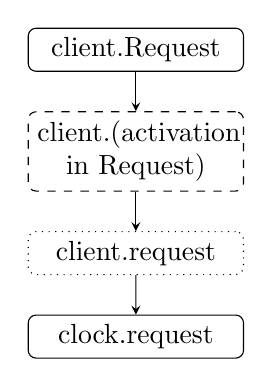
\begin{tikzpicture}[
    arrowstyle/.style={draw, -stealth},
    edge from parent/.style={draw, -stealth},
    reaction/.style={rectangle, draw, rounded corners=1mm, text width=2.5cm,
        text centered, anchor=north},
    activation/.style={rectangle, draw, rounded corners=1mm, dashed, text width=2.5cm,
        text centered, anchor=north},
    push/.style={rectangle, draw, rounded corners=1mm, dotted, text width=2.5cm,
        text centered, anchor=north},
    level 1/.style={sibling distance=7.0cm},
    level 2/.style={sibling distance=4.0cm},
    level 3/.style={sibling distance=3.0cm},
    level distance=0.5cm, growth parent anchor=south
]
\node (Action) [reaction] {client.Request}
  child {
    node (Activation01) [activation] {client.(activation in Request)}
    child {
      node (Push01) [push] {client.request}
      child {
        node (Reaction01) [reaction] {clock.request}
      }
    }
  }
;
\end{tikzpicture}
\endgroup
%%}%
\cprotect\caption{Transaction diagram for the \verb+client.Request+ action of the Clock System}
\label{request_transaction}
\end{figure}

\begin{figure}
\centering
%%\resizebox{\textwidth}{!}{%
\begingroup
\fontsize{10pt}{12pt}\selectfont
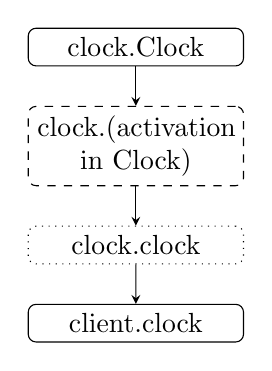
\begin{tikzpicture}[
    arrowstyle/.style={draw, -stealth},
    edge from parent/.style={draw, -stealth},
    reaction/.style={rectangle, draw, rounded corners=1mm, text width=2.5cm,
        text centered, anchor=north},
    activation/.style={rectangle, draw, rounded corners=1mm, dashed, text width=2.5cm,
        text centered, anchor=north},
    push/.style={rectangle, draw, rounded corners=1mm, dotted, text width=2.5cm,
        text centered, anchor=north},
    level 1/.style={sibling distance=7.0cm},
    level 2/.style={sibling distance=4.0cm},
    level 3/.style={sibling distance=3.0cm},
    level distance=0.5cm, growth parent anchor=south
]
\node (Action) [reaction] {clock.Clock}
  child {
    node (Activation01) [activation] {clock.(activation in Clock)}
    child {
      node (Push01) [push] {clock.clock}
      child {
        node (Reaction01) [reaction] {client.clock}
      }
    }
  }
;
\end{tikzpicture}
\endgroup
%%}%
\cprotect\caption{Transaction diagram for the \verb+clock.Clock+ action of the Clock System}
\label{clock_transaction}
\end{figure}

\section{Properties of Composition}
\label{propcomp}
In this section, we examine various features related to reactive components and composition.
Substitutional equivalence for reactive components is demonstrated by outlining a procedure for in-lining sub-components.
Hazards of composition, namely, non-deterministic state transitions resulting from conflicting and recursive composition, are identified and a means of detecting them is proposed.
The issue of decomposition is considered and \emph{pull ports} are introduced as a mechanism for decomposition.

\begin{figure}
\begin{verbatim}
component System {
  /* Substitution of clock component. */
  var int clock_counter (0)
  var bool clock_flag (false)
  push clock_clock(int t)

  reaction clock_request() clock_flag := true

  clock_Clock: clock_flag -> clock_flag := false activates clock_clock(clock_counter)

  clock_Tick: clock_counter := clock_counter + 1

  /* Substitution of client component. */
  var bool client_flag (false)
  push client_request()

  client_Request: !client_flag -> client_flag := true activates client_request()

  reaction client_clock(int t) client_flag := false || /* do something with t */

  bind {
    client_request -> clock_request
    clock_clock -> client_clock
  }
}
\end{verbatim}
\caption[Substitution of sub-components for the Clock System]{Substitution of state variables, ports, actions, and reactions for the sub-components of the System component of the Clock System}
\label{se1}
\end{figure}

\begin{figure}
\begin{verbatim}
component System {
  var int clock_counter (0)
  var bool clock_flag (false)
  var bool client_flag (false)
  push clock_clock(int t)
  push client_request()

  clock_Clock: clock_flag -> clock_flag, client_flag :=
    false, false activates clock_clock(clock_counter) ||
    /* do something with clock_counter */

  client_Request: !client_flag -> client_flag, clock_flag :=
    true, true activates client_request()

  clock_Tick: clock_counter := clock_counter + 1
}
\end{verbatim}
\caption[Simplification of expanded System component of the Clock System]{Simplifications of ports, bindings, and transitions in the expanded System component of the Clock System}
\label{se2}
\end{figure}

\subsection{Substitutional Equivalence}
\label{substitutional_equivalence}
For reactive components, substitutional equivalence means that a sub-component can be replaced with its definition and the result is a well-defined entity in the model.
To this end, a procedure for substituting the definition of a sub-component involves 1) renaming and adding all state variables, ports, actions, and reactions to the parent component and 2) simplifying bindings by substituting the transitions associated with a reaction into the action or reaction that activates the reaction in question.

To illustrate, Figure~\ref{se1} shows the result of substituting state variables, ports, actions, and reactions into the System component of Figure~\ref{system_component}.
Identifiers in the sub-components have been prefixed with the name of the sub-component instance to avoid name clashes.
For example, the \verb+request+ reaction in the \verb+clock+ sub-component has been renamed to \verb+clock_request+.
Figure~\ref{se2} shows the result of simplifying bindings and state transitions.
Note that the push ports have been retained for subsequent composition, i.e., the System component may be a component in a larger system.
The result is a reactive component whose ``size'' in terms of state variables, actions, and reactions is the sum of the sizes  of its constituent components.
Substituting the definition of the Clock component and Client components into the System component confirms the intuition that the flag variable in the client and flag variable in the clock are the same since 1) initially they have the same value and 2) they take on the same value in every state transition.

\subsection{Determinism and Composition}
\label{determinism}

\begin{figure}
\centering
%%\resizebox{\textwidth}{!}{%
\begingroup
\fontsize{10pt}{12pt}\selectfont
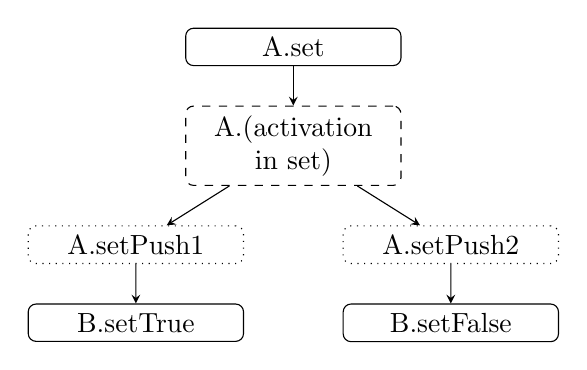
\begin{tikzpicture}[
    arrowstyle/.style={draw, -stealth},
    edge from parent/.style={draw, -stealth},
    reaction/.style={rectangle, draw, rounded corners=1mm, text width=2.5cm,
        text centered, anchor=north},
    activation/.style={rectangle, draw, rounded corners=1mm, dashed, text width=2.5cm,
        text centered, anchor=north},
    push/.style={rectangle, draw, rounded corners=1mm, dotted, text width=2.5cm,
        text centered, anchor=north},
    level 1/.style={sibling distance=7.0cm},
    level 2/.style={sibling distance=4.0cm},
    level 3/.style={sibling distance=3.0cm},
    level distance=0.5cm, growth parent anchor=south
]
\node (Action) [reaction] {A.set}
  child {
    node (Activation01) [activation] {A.(activation in set)}
    child {
      node (Push01) [push] {A.setPush1}
      child {
        node (Reaction01) [reaction] {B.setTrue}
      }
    }
    child {
      node (Push02) [push] {A.setPush2}
      child {
        node (Reaction02) [reaction] {B.setFalse}
      }
    }
  }
;
\end{tikzpicture}
\endgroup
%%}%
\caption{Transaction diagram for a non-deterministic transaction}
\label{ndt}
\end{figure}

The result of composing two well-defined reactive components may yield a system that is non-deterministic.
The two ``hazards'' that must be avoided are non-deterministic assignment to state variables and recursively activated reactions.
Non-deterministic assignment results when the next value for a state variable is not well defined due to the inclusion of two or more transitions in a transaction that operate on the state variable.
To illustrate, consider the transaction depicted in Figure~\ref{ndt}.
The set action of component A has a single activation that activates both the setPush1 and setPush2 push ports.
The setPush1 port is bound to the setTrue reaction of component B while the setPush2 port is bound to the setFalse reaction of the same component B.
Suppose that the setTrue reaction sets a flag to true while the setFalse reaction sets the same flag to false.
The transaction is non-deterministic because the value of the flag after the (A,set) transaction may either be true or false.
An offending pair of transitions may appear anywhere in a transaction graph given that arbitrary transaction graphs may be constructed through composition.
If the underlying language used to define transitions admits pointers, dynamic memory, if statements, and loops (i.e., is Turing-complete), then the problem of determining if two transitions operate on the same state variable is undecidable in general~\cite{Landi:1992:USA:161494.161501, Ramalingam:1994:UA:186025.186041}.
For a transaction graph $G$, instances $i_1$ and $i_2$, and actions/reactions $t_1$ and $t_2$, a necessary (but not sufficient) condition for non-deterministic assignment $\mathit{NDA}$ from composition is $\mathit{NDA}(G): \exists (i_1, t_1), (i_2, t_2) \in G.N, i_1 = i_2, t_1 \ne t_2$ which says that the transaction must contain two different transitions involving the same component instance.

A recursively activated transition occurs when the transaction graph has a cycle.
The execution of such a transaction may result in well-defined next values for all state variables assuming that 1)~the recursion is bounded and 2)~the parameters passed to every reaction result in identical computations.
A transaction may be analyzed like a traditional transformational program since it has finite input, a finite output, and should terminate.
The first problem, then, is a thinly disguised version of the halting problem since it asks if a computation (the transaction) expressed in a Turing-complete language terminates (has bounded recursion)~\cite{Turing01011937, davis1958computability}.
A bounded recursion means that the execution of the transaction will generate a bounded number of activations $A$.
For each activation $a \in A$, we must determine what state is updated by $a$.
If the language is Turing-complete, then this problem is undecidable in general~\cite{Landi:1992:USA:161494.161501, Ramalingam:1994:UA:186025.186041}.
For state variables that are updated by more than one activation, we must then show that each activation sets the state variable to the exact same next state.
If we treat each activation as a program, then we require a function that determines if two (arbitrary) programs compute the same function, which is again, undecidable in general~\cite{Rice:53}.

The difficulty of detecting composition that results in non-deterministic assignments suggests that these problems are best checked by a machine.
That is, an implementation of reactive components may prevent non-deterministic assignment by checking that $\mathit{NDA}(G)$ is false for all transaction graphs in the system.
Similarly, an implementation may check for recursive activation by checking for cycles in transaction graphs.
Both of these approaches are used by the implementation described in Section~\ref{sound_composition}.

\subsection{Decomposition, Getters, and Pull Ports}
\label{decomposition}
Substitutional equivalence implies that the process of substituting the definition of a sub-component into a parent component may be reversed and that sub-components may be ``factored out'' of an existing component, e.g., for reuse with other components.
%% One motivation for extracting sub-components is to support the software engineering practice of refactoring where common code is extracted so that it can be reused in various places.

Another motivation for decomposition is potentially increased performance through parallelism.
Recall that true concurrency in reactive components is modeled as the serial and non-deterministic execution of atomic actions.
Two transactions can be safely executed concurrently if it can be shown that the state variables involved in each transaction are disjoint.
As was previously mentioned, making this determination is undecidable for Turing-complete languages in the general case.
However, the problem becomes decidable if the component instance is used as a proxy for its constituent state variables.
Let $\mathit{rw}: t \to \{ \mathit{Read}, \mathit{Write} \}$ be a function that maps a transition to a value indicating that variables are read-only during the transition or written in some way.
Two instance/transition pairs are independent ($\mathit{indp}$) if either the instances are different or at most one of the transitions writes to the variables of the instance:
\begin{equation}
\mathit{indp}((i_1, t_1), (i_2, t_2)): i_1 \ne i_2 \lor \lnot (\mathit{rw}(t_1) = \mathit{Write} \land \mathit{rw}(t_2) = \mathit{Write})
\end{equation}
Two transaction graphs are independent if all of their nodes are independent $\mathit{indp}(G_1, G_2) = \forall (i_1, t_1) \in G_1.N, (i_2, t_2) \in G_2.N \; \mathit{indp}((i_1, t_1), (i_2, t_2))$.
The significance of the preceding analysis is that the determination about what actions can be executed concurrently becomes machine checkable due to the strong guarantee that state variables belonging to an instance can only be modified by the transitions of that instance.

To illustrate the mechanisms required for decomposition, we will factor out a Counter component from the Clock component of Figure~\ref{clock_component} and then rewrite the Clock component using the Counter component.
Upon inspection, the \verb+Tick+ action and \verb+request+ reaction can be executed concurrently since the state variables involved in each transition are disjoint.
Figure~\ref{counter_component} shows the Counter component which consists of a \verb+counter+ state variable.
The \verb+Tick+ action can be moved to the Counter component without complication.
The \verb+Clock+ action of the Clock component \emph{reads} the value of \verb+counter+ which suggests that a mechanism for accessing the state variables in a component is required.
Thus, we introduce the notion of a \emph{getter} method which can be called on a component to produce a value that may be derived from its state variables.
In the Counter component, the \verb+getCounter+ getter returns the current value of the counter.
A getter is not allowed to modify the state of a component and may only be invoked in the immutable phase.
These semantics preserve the strict separation of immutable phase and mutable phase.
When analyzing composition, a getter is treated like a transition that reads the state variable of the corresponding instance.
Figure~\ref{factored_clock_component} shows the Clock component rewritten to use a Counter sub-component and a getter.

\begin{figure}
\begin{verbatim}
component Counter {
  var int counter (0)

  Tick: counter := counter + 1

  getCounter() int {
    return counter
  }
}
\end{verbatim}
\caption{Definition of the Counter component of the Factored Clock System}
\label{counter_component}
\end{figure}

\begin{figure}
\begin{verbatim}
component Clock {
  var Counter c
  var bool flag (false)
  push clock(int t)

  reaction request() flag := true

  Clock: flag -> flag := false activates clock(c.getCounter())
}
\end{verbatim}
\caption{Definition of the Clock component of the Factored Clock System}
\label{factored_clock_component}
\end{figure}

The logic associated with the \verb+flag+ state variable represents a generic request-response protocol except for the call to \verb+c.getCounter()+.
To indirect the call to \verb+c.getCounter()+ we introduce the notion of a \emph{pull port}.
A pull port represents an external value dependency.
A component can demand a value from the pull port in the immutable phase.
Like push ports, pull ports have an active and passive side.
The active side represents the caller and the passive side represents the callee.
Getters are sufficient to realize the passive side of a pull port.
Every active pull port must be bound to exactly one passive pull port via composition.
Figure~\ref{request_response_component} shows a component that implements the request-response protocol using a pull port \verb+getValue+.
Figure~\ref{factored2_clock_component} shows the Clock component written in terms of the Counter and RequestResponse components.
An \verb+export+ directive allows reactions, getters, and ports in sub-components to be available in the interface of the encapsulating component.

\begin{figure}
\begin{verbatim}
component RequestResponse {
  var bool flag (false)
  pull getValue() int
  push response(int t)

  reaction request() flag := true

  Response: flag -> flag := false activates response(getValue())
}
\end{verbatim}
\caption{Definition of the RequestResponse component of the Factored Clock System}
\label{request_response_component}
\end{figure}

\begin{figure}
\begin{verbatim}
component Clock {
  var Counter c
  var RequestResponse rr
  push request()
  push clock(int t)

  bind {
    c.getCounter -> rr.getValue
  }

  export rr.request as request
  export rr.response as clock
}
\end{verbatim}
\caption{Definition of the Clock component of the Factored Clock System (fully-factored)}
\label{factored2_clock_component}
\end{figure}

Pull ports are subject to a hazard of composition similar to the recursive activation hazard of push ports.
A cycle in the graph of composed pull ports is equivalent to a recursively defined function.
The recursion may be bounded but this is undecidable in the general case.
Consequently, an implementation may reject recursively defined getters and pull ports.

\section{Summary}
In this chapter, we have presented the reactive component model for reactive programs.
A reactive component consists of a set of state variables and transitions that are private to the component.
The interface of a reactive component consists of push ports and reactions, which allow a component to trigger a transition in another component, and pull ports and getters, which allow a component to access the state of another component.
The external or visible behavior of a reactive component can be traced through its interface, specifically its push ports.
The internal details of a component can often be abstracted away to permit reasoning about the behavior of a composed system at various levels of detail.
Composition is achieved through recursive encapsulation (sub-components) and explicit port binding and satisfies the requirements for principled composition set forth in Section~\ref{challenges}.
As demonstrated in Section~\ref{substitutional_equivalence}, the definitions of sub-components can be substituted into the containing component resulting in an equivalent system (substitutional equivalence).
Similarly, sub-components may be ``factored out'' by using pull ports and getters to safely access the state of the sub-components.

The private nature of state variables and transitions causes properties established from the text of a component to be preserved through composition.
Composition links transitions to form an atomic transaction that allows the properties of one component to be related to another component.
When the sub-components of a component are protected from further composition, the properties derived from their interactions are preserved as the parent component is composed.
Property-preserving composition is essential for reasoning about systems in a hierarchical and/or modular fashion.

The result of composing reactive components is either well-defined due to the atomic nature of transactions or illegal due to the composition hazards of recursive transactions and non-deterministic state transitions.
Analysis of these hazards at the state variable level is impossible due to the undecidable nature of their sub-problems.
This suggests that implementations may restrict composition to prevent the conditions necessary for recursive transactions and non-deterministic state transitions.
The main concession is allowing a component instance to proxy for its state variables.
The problem of detecting recursive transactions, then, can be posed as the problem of detecting cycles in a directed graph.
Similarly, the problem of detecting potentially non-deterministic state transitions is reduced to a set membership problem.
Valid systems that fail the check for non-deterministic state transitions using component instance proxies can be refactored by decomposing  the offending components.

     }%
        &
        {\center
\lstset{
  language={rcgo},
  basicstyle=\tiny\ttfamily,
  columns=fixed,
}

\begin{lstlisting}
type Clock component {
  counter uint;
  flag bool;
  response push (t uint);
};
...
\end{lstlisting}
}

        \\
        \hline
        \rcgo{} Platform & \rcgo{} Scheduler \\

\begin{center}
\resizebox{.25\textwidth}{!}{%
\begingroup
\fontsize{10pt}{12pt}\selectfont
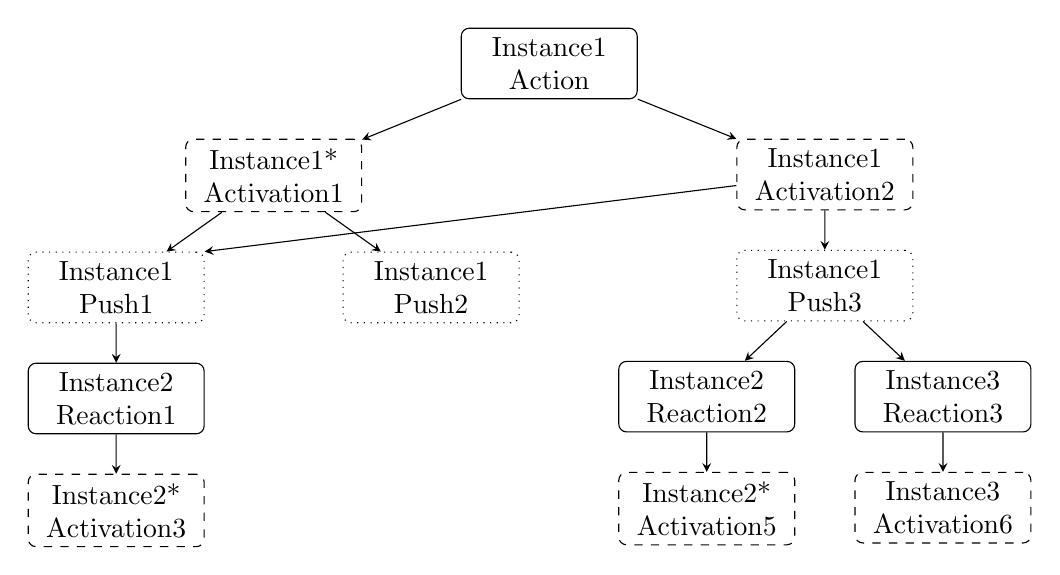
\begin{tikzpicture}[
    arrowstyle/.style={draw, -stealth},
    edge from parent/.style={draw, -stealth},
    reaction/.style={rectangle, draw, rounded corners=1mm, text width=2cm,
        text centered, anchor=north},
    activation/.style={rectangle, draw, rounded corners=1mm, dashed, text width=2cm,
        text centered, anchor=north},
    push/.style={rectangle, draw, rounded corners=1mm, dotted, text width=2cm,
        text centered, anchor=north},
    level 1/.style={sibling distance=7.0cm},
    level 2/.style={sibling distance=4.0cm},
    level 3/.style={sibling distance=3.0cm},
    level distance=0.5cm, growth parent anchor=south
]
\node (Action) [reaction] {Instance1 Action}
  child {
    node (Activation01) [activation] {Instance1* Activation1}
    child {
      node (Push01) [push] {Instance1 Push1}
      child {
        node (Reaction01) [reaction] {Instance2 Reaction1}
        child {
          node (Activation03) [activation] {Instance2* Activation3}
        }
      }
    }
    child {
      node (Push02) [push] {Instance1 Push2}
    }
  }
  child {
    node (Activation02) [activation] {Instance1 Activation2}
    child {
      node (Push03) [push] {Instance1 Push3}
      child {
        node (Reaction02) [reaction] {Instance2 Reaction2}
        child {
          node (Activation04) [activation] {Instance2* Activation5}
        }
      }
      child {
        node (Reaction03) [reaction] {Instance3 Reaction3}
        child {
          node (Activation05) [activation] {Instance3 Activation6}
        }
      }
    }
  }
;

\draw[arrowstyle] (Activation02) -- (Push01.north east);

\end{tikzpicture}
\endgroup
}%
\end{center}
&
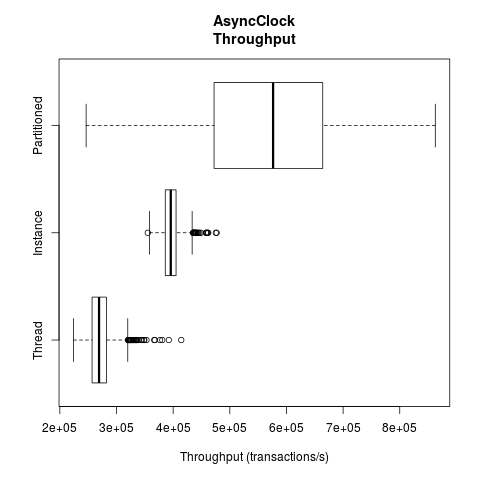
\includegraphics[width=.25\textwidth]{async_throughput_box.png}
\\
        \hline
  \end{tabular}


\end{frame}

%% \begin{frame}{Preliminaries}
%%   \centering

%%     \resizebox{\textwidth}{!}{
%%     \begin{tikzpicture}
%%       [>=stealth',
%%         line/.style={draw, thick, ->},
%%         entity/.style={
%%           rectangle,
%%           rounded corners,
%%           draw=black, very thick,
%%           text centered,
%%           text width=6em,
%%           minimum height=8em,
%% }]
%%       \node[entity, label={Environment}] (environment) {};
%%       \node[entity, right=4cm, label={Program}] (program) at (environment) {};
%%       \draw[line] ($(environment.south east)!0.66!(environment.north east)$) -- ($(program.south west)!0.66!(program.north west)$) node [midway, above] {Input};
%%       \draw[line] ($(program.south west)!0.33!(program.north west)$) -- ($(environment.south east)!0.33!(environment.north east)$) node [midway, below] {Output};

%%       \draw[line,
%%         decoration={markings, mark=at position 0.0 with {\arrow{<}}},
%%         postaction={decorate}
%%       ]
%%       (program) circle (0.5) node [label={[label distance=.3cm]90:Processing}] {};
%%     \end{tikzpicture}
%%     }

%%     \begin{itemize}
%%     \item Output/input is atomic
%%     \item Interface consists of input/output structures
%%     \item Processing/output is sporadic
%%     \end{itemize}

%% \end{frame}

\begin{frame}{The Reactive Components Model}
  \centering

  \vspace*{24pt}

        \resizebox{\textwidth}{!}{%
          \chapter{Reactive Component Model}
\label{model}

In this chapter, we present a new model for composing and decomposing reactive programs via \emph{reactive components}.
The model is biased toward practical software development even as it enforces properties based in formal methods.
Consequently, the model favors utility, practicality, flexibility, and ease of implementation.
Unlike UNITY in which composition is not property-preserving, the composition of reactive components is property-preserving which facilitates hierarchical and modular reasoning.
Unlike I/O Automata in which transitions have limited depth, a transition among reactive components may access and cascade to an arbitrary number of other components, which permits decomposition to an arbitrary depth and degree.

%% \paragraph{Formal models and software engineering.}
%% I claim that most of the software that is ``put into production'' will never be proved formally correct.
%% This is a function of economics since modeling and constructing proofs is a labor-intensive process that can only be justified for safety or mission critical software.
%% However, I would argue that the development and application of formal models are critical to software engineering.
%% To illustrate, consider \emph{structured programming}~\cite{dahl1972structured}.
%% Structured programming assumes an abstract machine that executes programs that are restricted to a small set of well-defined control structures and assignment statements.
%% A program written in this form can be reasoned about directly from the text by formulating a Hoare-triple for each statement.
%% Structured programming opened the door for \emph{structured programming languages} which are also based on well-defined control structures and evaluation semantics.
%% Thus, while very few programmers will prove their structured programs correct, all of them informally use structured programming when they are fixing a bug revealed by a unit test or analyzing a core dump in a debugger.
%% Structured programming languages reduced the accidental complexity associated with writing the same program in assembly language.

%% The realm of reactive programs is waiting for a similar reduction in accidental complexity.
%% Taking a hint from structured programming, I believe two things are required.
%% First, we must write reactive programs against an easy-to-reason-about abstract machine instead of low-level interfaces like atomic instructions and thread libraries.
%% Second, we must restrict the form of reactive programs so that they can be reasoned about from the text.
%% I hope the proposed model of reactive systems is a step toward toward this goal.

\section{Features of the Model}

%% left active pull port
%% x, y, width, height, label
\def\lapull[#1,#2,#3,#4,#5,#6]#7{
  \draw [fill=lightgray] (#1,#2) -- ++(${#4*.5}*(-1,0) + {#4*.5}*(0,-1)$) -- ++($#3*(1,0)$) -- ++($#4*(0,1)$) -- ++($#3*(-1,0)$) -- cycle;
  \node (#5) at (#1,#2) {};
  \node (#6) at ($(#1,#2) + {#3 - .5 * #4}*(1,0)$) {};
  \node [right, align=left] at (#1,#2) {#7};
}

%% left active push port
%% x, y, width, height, label
\def\lapush[#1,#2,#3,#4,#5,#6]#7{
  \draw [fill=white] ($(#1,#2) + {#4*.5}*(-1,0)$) -- ++(${#4*.5}*(1,0) + {#4*.5}*(0,-1)$) -- ++($#3*(1,0)$) -- ++($#4*(0,1)$) -- ++($#3*(-1,0)$) -- cycle;
  \node (#5) at ($(#1,#2) - .5*#4*(1,0)$) {};
  \node (#6) at ($(#1,#2) + {#3}*(1,0)$) {};
  \node [right, align=left] at (#1,#2) {#7};
}

%% left passive pull port
%% x, y, width, height, label
\def\lppull[#1,#2,#3,#4,#5,#6]#7{
  \draw [fill=lightgray] ($(#1,#2) + {#4*.5}*(-1,0)$) -- ++(${#4*.5}*(1,0) + {#4*.5}*(0,-1)$) -- ++($#3*(1,0)$) -- ++($#4*(0,1)$) -- ++($#3*(-1,0)$) -- cycle;
  \node (#5) at ($(#1,#2) - .5*#4*(1,0)$) {};
  \node (#6) at ($(#1,#2) + {#3}*(1,0)$) {};
  \node [right, align=left] at (#1,#2) {#7};
}

%% left passive push port
%% x, y, width, height, label
\def\lppush[#1,#2,#3,#4,#5,#6]#7{
  \draw [fill=white] (#1,#2) -- ++(${#4*.5}*(-1,0) + {#4*.5}*(0,-1)$) -- ++($#3*(1,0)$) -- ++($#4*(0,1)$) -- ++($#3*(-1,0)$) -- cycle;
  \node (#5) at (#1,#2) {};
  \node (#6) at ($(#1,#2) + {#3 - .5*#4}*(1,0)$) {};
  \node [right, align=left] at (#1,#2) {#7};
}

%% right passive pull port
%% x, y, width, height, label
\def\rppull[#1,#2,#3,#4,#5,#6]#7{
  \draw [fill=lightgray] ($(#1,#2) + {#4*.5}*(1,0)$) -- ++(${#4*.5}*(-1,0) + {#4*.5}*(0,-1)$) -- ++($#3*(-1,0)$) -- ++($#4*(0,1)$) -- ++($#3*(1,0)$) -- cycle;
  \node (#5) at ($(#1,#2) + {#4*.5}*(1,0)$) {};
  \node (#6) at ($(#1,#2) + {#3}*(-1,0)$) {};
  \node [left] at (#1,#2) {#7};
}

%% right active push port
%% x, y, width, height, label
\def\rapush[#1,#2,#3,#4,#5,#6]#7{
  \draw [fill=white] ($(#1,#2) + {#4*.5}*(1,0)$) -- ++(${#4*.5}*(-1,0) + {#4*.5}*(0,-1)$) -- ++($#3*(-1,0)$) -- ++($#4*(0,1)$) -- ++($#3*(1,0)$) -- cycle;
  \node (#5) at ($(#1,#2) + {#4*.5}*(1,0)$) {};
  \node (#6) at ($(#1,#2) + {#3}*(-1,0)$) {};
  \node [left] at (#1,#2) {#7};
}

%% right passive push port
%% x, y, width, height, label
\def\rppush[#1,#2,#3,#4,#5,#6]#7{
  \draw [fill=white] (#1,#2) -- ++(${#4*.5}*(1,0) + {#4*.5}*(0,-1)$) -- ++($#3*(-1,0)$) -- ++($#4*(0,1)$) -- ++($#3*(1,0)$) -- cycle;
  \node (#5) at (#1,#2) {};
  \node (#6) at ($(#1,#2) + {#3 - .5*#4}*(-1,0)$) {};
  \node [left] at (#1,#2) {#7};
}

%% right active pull port
%% x, y, width, height, label
\def\rapull[#1,#2,#3,#4,#5,#6]#7{
  \draw [fill=lightgray] (#1,#2) -- ++(${#4*.5}*(1,0) + {#4*.5}*(0,-1)$) -- ++($#3*(-1,0)$) -- ++($#4*(0,1)$) -- ++($#3*(1,0)$) -- cycle;
  \node (#5) at (#1,#2) {};
  \node (#6) at ($(#1,#2) + {#3 - .5*#4}*(-1,0)$) {};
  \node [left] at (#1,#2) {#7};
}

\begin{figure}[H]
\centering
\resizebox{\textwidth}{!}{%
\begingroup
\fontsize{10pt}{12pt}\selectfont
\begin{tikzpicture}
[
arrowstyle/.style={
  decoration={markings,mark=at position 1 with {\arrow[scale=2,]{stealth}}},
  postaction={decorate},
  shorten >=0.4pt
}
]

%% component boundary
\draw (0,0) rectangle (10,8.25);
%% active pull ports
\lapull[0,1.5,1,.5,apullex1,apullin1]{}
\node[align=center] at (-1,1.5) {active\\pull port};
\lapull[0,.5,1,.5,apullex2,apullin2]{}
%% passive pull ports
\rppull[10,1.5,1,.5,ppullex1,ppullin1]{}
\node[align=center] at (11,1.5) {passive\\pull port};
\rppull[10,.5,1,.5,ppullex2,ppullin2]{}
\draw[thick] (apullin2.center) -- (ppullin2.center);
%% actions and rections
\node[draw, diamond, minimum height=15, minimum width=20] (pre) at (2.5,3) {};
\node at (2.5,2.5) {precondition};
\node[draw, minimum height=15, minimum width=50, rounded corners=5] (trans1) at (5,3) {};
\draw[dashed] (3.5,3) ellipse (3 and 1);
\node at (3.5,3.5) {\textbf{\emph{action}}};
\node[draw, minimum height=15, minimum width=50, rounded corners=5] (trans2) at (5,5) {};
\node at (5,4.5) {transition};
\draw[thick,arrowstyle] (pre) -- (trans1);
\draw[thick] (apullin1.center) -| (trans1) node[pos=.5,right] {\textbf{call}};
%% active push ports
\rapush[10,3,1,.5,apushex1,apushin1]{}
\rapush[10,4,1,.5,apushex2,apushin2]{}
\rapush[10,5,1,.5,apushex3,apushin3]{}
\node[align=center] at (11.1,5) {active\\push port};
\draw[thick,dashed,arrowstyle] (trans1) -- (apushin1.center);
\draw[thick,dashed,arrowstyle] (trans1) -- (apushin2.center);
\node at(7.5,4) {\textbf{activate}};
\draw[thick,dashed,arrowstyle] (trans2) -- (apushin2.center);
\draw[thick,dashed,arrowstyle] (trans2) -- (apushin3.center);
%% passive push ports
\lppush[0,5,1,.5,ppushex1,ppushin1]{}
\draw[thick,arrowstyle] (ppushin1.center) -- (trans2);
\node[align=center] at (-1.1,5) {passive\\push port};
\draw[dashed] (2,5) ellipse (5 and 1);
\node at (2,5.5) {\textbf{\emph{reaction}}};
\node[draw, cylinder, shape border rotate=90, minimum height=40, minimum width=40] (sv1) at (5,7.25) {};
\node[align=center] at (5,6.25) {state variables};
\end{tikzpicture}
\endgroup
}%
\caption{Features of a reactive component\label{reactive_component}}
\end{figure}

Figure~\ref{reactive_component} shows the major features of a reactive component.
As in other state-based formal models like UNITY~\cite{chandy1989parallel} and I/O Automata~\cite{nancy1996distributed}, the core of a reactive component in this model is a set of \emph{state variables} and a set of atomic \emph{transitions} that manipulate those state variables.
When reasoning about a system, behavior is expressed as propositions over the state variables where the propositions are derived from the transitions.

%% The contribution that this work makes to existing state-based formal models of reactive systems is a combination of interface elements and composition semantics that allow reactive programs to be composed in a principled way.

The reactive component model defines interface elements and composition semantics that allow reactive programs to be composed in a principled way.
For example, an \emph{active push port} allows a transition in one component to be linked to a transition in another component such that the resulting combined transition is atomic.
Active push ports allow reactive components to publicize their behavior.
An active push port may be \emph{bound} to and conditionally \emph{activate} zero or more \emph{passive push ports}.
A passive push port names the corresponding transition that will be executed when the passive push port is activated.
This combination of passive push port and transition is called a \emph{reaction} because it reacts to a transition in another component.

The atomic linkage of a transition in one component to a transition in another component through the push port mechanism allows the properties of each component to be related to one another and more complex systems to be constructed by composing simpler systems.
Transitions that are not executed via a passive push port are executed by the scheduler.
A transition of this kind may be governed by a Boolean expression called a \emph{precondition}.
The combination of a precondition and transition is called an \emph{action} because it is a voluntary transition under the control of the containing component.

An \emph{active pull port} represents an immutable external data dependency.
The component may \emph{call} an active pull port to yield a value required in a transition.
Active pull ports must be bound to a \emph{passive pull port} which resembles a function returning a value, e.g., a getter or a predicate.
Where push ports allow components to publicize their behavior, pull ports allow components to safely publicize their internal state for use by other components.

Composition in the reactive component model has two main features.
The first is recursive encapsulation where a state variable in one component may represent an instance of another reactive component.
The second is the ability to bind push ports and pull ports through an \emph{explicit} set of \emph{bindings}.
The decision to use an explicit set of bindings (as opposed to implicit named-based matching) is more in keeping with the goals and techniques of practical software development, since it facilitates the use of software developed under different naming conventions, i.e., third-party software.
A third minor feature called \emph{exporting} is the ability of an encapsulating component to adopt interface elements of its sub-components without defining complimentary ports and transitions that do nothing but forward an activation or call.
The ability to publicize behavior and state and the ability to assemble well-defined behavior from existing behaviors in a straight-forward and flexible way are thus defining characteristics of the reactive component model.

\begin{figure}
\centering
\resizebox{\textwidth}{!}{%
\begingroup
\fontsize{10pt}{12pt}\selectfont
\begin{tikzpicture}
\draw (0,6.5) rectangle (5,10);
\node[below] at (2.5,10) {Web Server};
\rapull[5,9,3.4,.5,ex1a,ignore]{verify(HttpHeader)};
\rapush[5,8,3.6,.5,ex2a,ignore]{request(HttpRequest)};
\rppush[5,7,4.2,.5,ex3a,ignore]{respond(HttpResponse)};

\draw(6,2.5) rectangle (11,10);
\node[below] at (8.5,10) {Application Logic};
\lppull[6,9,3.4,.5,ex1b,ignore]{verify(HttpHeader)};
\lppush[6,8,3.8,.5,ex2b,ignore]{request(HttpRequest)};
\lapush[6,7,3.9,.5,ex3b,ignore]{respond(HttpResponse)};

\rapush[11,6,3.5,.5,ex4a,ignore]{request(DBRequest)};
\rppush[11,5,4.1,.5,ex5a,ignore]{respond(DBResponse)};

\rapush[11,3,2.4,.5,ex6a,ignore]{log(Message)};

\draw (12,4.5) rectangle (17,7);
\node[below] at (14.5,7) {Database};
\lppush[12,6,3.7,.5,ex4b,ignore]{request(DBRequest)};
\lapush[12,5,3.8,.5,ex5b,ignore]{respond(DBResponse)};

\draw (12,2.5) rectangle (17,4);
\node[below] at (14.5,4) {Logging Service};
\lppush[12,3,2.5,.5,ex6b,ignore]{log(Message)};

\draw (ex1a.center) -- (ex1b.center);
\draw (ex2a.center) -- (ex2b.center);
\draw (ex3a.center) -- (ex3b.center);
\draw (ex4a.center) -- (ex4b.center);
\draw (ex5a.center) -- (ex5b.center);
\draw (ex6a.center) -- (ex6b.center);

\end{tikzpicture}
\endgroup
}%
\caption{Diagram of a web application built using reactive components\label{web_server}}
\end{figure}

To demonstrate the utility of component interfaces and explicit support for property-preserving composition, we now present an illustrative design for a web application using reactive components, as is shown in Figure~\ref{web_server}.
The web application consists of five reactive components.
The first is an unnamed top-level component representing the complete application.
This component has four sub-components representing a web server, the application logic, a database, and a logging service.
The ports of the application logic component have been bound to the corresponding ports in the web server, database, and logging service components.
The interface of a component, which consists of its ports, provides insight into the behavior of the component.
For example, based on the interface of the web server component we may expect it to 1)~verify incoming HTTP requests\footnote{A production web server may verify that the requested HTTP method can be applied to the given URI, that content length limits are respected, that content types are supported, etc.}, 2)~pass on valid HTTP requests to the application, and 3)~accept HTTP responses from the application.

Figure~\ref{web_server} also demonstrates how reactive programs can be constructed by composing reactive components, so that a developer may focus on the application logic and use existing components for the web server, database, and logging service.
Furthermore, one can imagine developing three stateless components surrounding the application logic that do nothing but translate messages between application specific message types and the generic types required by the web server, database, and logging service.
The application logic, then, is completely isolated from the surrounding libraries and may be tested by providing mock components for the web server, database, and logging service.
The application logic itself has a well-defined interface and could be reused, say, by implementing a graphical front-end to drive the application instead of a web service.

\subsection{State Variables}
Part of the internal core of a reactive component is a set of state variables, which are the subject of the propositions that demonstrate the behavior of the system.
The state variables are manipulated by the assignment statements that constitute the transitions.
As in other formal models, the types of the state variables may be selected to make writing proofs easier.
%% That is, the state variables have mathematically friendly types like integers, sets, and lists.
However, implementations of the reactive component model must provide a concrete type system that allows the state variables to be realized on a given machine.
For example, the \rcgo{} language for reactive components presented in Chapter~\ref{language} of this dissertation uses the type system of Go to define the types of state variables.
The type of a state variable also may be a reactive component type, which facilitates recursive encapsulation.
For modeling purposes, state variables typically have \emph{value semantics} to avoid reasoning about references and aliasing.
However, and as a practical concession, we will introduce pointers for building arbitrary linked data structures (since we advocate an imperative state-based implementation) and discuss issues raised by introducing pointers into the reactive component model in Chapter~\ref{language}.

\subsection{Atomic State Transitions}
The rest of the internal core of a reactive component is a set of atomic state transitions that manipulate the state variables.
A precise definition of the atomicity of state transitions will be deferred to the subsequent sections on composition (Section~\ref{composition}) and execution (Section~\ref{execution}).
State variables and state transitions are private, meaning that transitions can only refer to the state variables of the associated reactive component and a transition in one reactive component can only be linked to a transition in another component through the composition mechanisms.
Thus, all initialization and updates to state variables can be determined by examining the transitions of the corresponding component.
The encapsulation of state variables contribute to composition being \emph{compositional}.
All properties established from the transitions of a component will continue to hold as the component participates in composition since the set of transitions that affect the state variables is fixed.
State transitions must be deterministic meaning that the next value of every state variable is uniquely and well defined.
State transitions defined by a sequence of simple assignments are implicitly deterministic.
However, special care must be take to ensure that state transitions are deterministic when described using parallel assignment statements as the same variable may appear on the left-hand-side and be assigned two different values~\cite{chandy1989parallel}.
As described in Sections~\ref{composition} and \ref{execution}, composition links transitions using parallel assignment which creates an opportunity for non-deterministic state transitions.
The problem of non-deterministic state transitions arising from composition is explored in Section~\ref{propcomp}.

The reactive component model presented in this chapter does not prescribe a specific language for encoding state transitions.
The language used depends on the goals and tastes of the one developing or analyzing the model.
For example, expressing transitions using the programming language of UNITY~\cite{chandy1989parallel} may allow the modeler to extract proofs from the text, a major goal of UNITY.
The approach used by I/O Automata~\cite{nancy1996distributed} is to specify the condition established by each transition.
As with state variables, we present a language that uses the statements and expressions of the Go programming language to encode state transitions in Chapter~\ref{language}.
This furthers our goal of making reactive components approachable by a general software engineering audience.
%% from Dr. Gill
%% which aims to allow models to be incorporated directly into standard software environments.
%% This isn't accurate.  Compatibility with existing software is not the goal nor should it be a goal as existing software is based on threads which cannot reasonably be integrated with reactive components.

\subsection{Actions, Reactions, Push Ports, Bindings, and Composition}
\label{composition}
A state transition is either part of an action or a reaction.
An \emph{action} is a state transition whose execution is under the control of the component to which it belongs.
The action is guarded by a \emph{precondition} that is guaranteed to be true the instant before the action is executed.
The precondition is a Boolean expression that determines if the action is \emph{enabled} or \emph{disabled}.
If the precondition is absent, it is assumed to be true.

A \emph{reaction} is a state transition whose execution is under the control of another action or reaction.
Thus, we require a mechanism for linking a reaction to an action or another reaction.
To do this, we introduce the notion of a \emph{push port}.
A push port is a typed interaction point consisting of an active side that conditionally \emph{activates} the port and provides arguments to the port, and a passive side that \emph{reacts} to the port and may access the arguments provided by the active side.
A reaction, therefore, is the combination of a passive push port and a state transition.

A \emph{binding} is a declaration that associates an active push port in one component with a reaction in another component.
The transition associated with the reaction is executed atomically with the transition that activates the active push port.
Composition in the reactive component model is achieved by declaring sub-components (recursive encapsulation) and linking transitions via binding.

\subsection{Transactions}

A \emph{transaction} is a compound and concrete state transition formed by expanding the activations in an instance/action pair, subject to the bindings in a system.
The instance and action that define a transaction are called the \emph{root} of the transaction.
A transaction is enabled/disabled if its root action is enabled/disabled.
Given the root instance and action, we may enumerate the active push ports that may be activated by the transition of the action.
Note that the activation of a push port is conditional, being under the control of the transition.
The push ports, in turn, activate reactions in particular component instances.
The transitions associated with the reactions may activate other push ports and so on.
This analysis can be repeated to discover all of the reactions that are linked to the root action.
The result is a \emph{transaction graph} which is a directed acyclic graph $G = (N,E)$.
Each node $n \in N$ is a pair $(i, x)$ where $i$ is a component instance and $x$ is either an action, reaction, activation, or push port.
Each edge $e \in E$ corresponds to a causal relationship between an action/reaction and an activation, an activation and a push port, or a push port and a reaction.
The edges between actions/reactions and activations indicate that the action/reaction \emph{may} execute the activation, as they may be conditionally executed.
The edges between activations and push ports and between push ports and reactions indicate that the implied push port or reaction \emph{will} be executed if the upstream activation is executed.

\subsection{Execution}
\label{execution}
We adopt the common practice of modeling concurrency with non-deterministically executed atomic actions as is done in UNITY~\cite{chandy1989parallel}, I/O Automata~\cite{nancy1996distributed}, and the Actor Model~\cite{agha1985actors}.
The execution of transactions is performed by a \emph{scheduler}.
The scheduler executes one transaction at a time, thus, each transaction is \emph{atomic} with respect to all other transactions.
A transaction is \emph{enabled} if its precondition is true.
When executing a transaction, the scheduler first evaluates the precondition and then executes the body of the transaction if the transaction is enabled.
Thus, executing an enabled transaction \emph{may} result in a state change while executing a disabled transaction \emph{never} causes a state change.
The scheduler is \emph{fair} meaning that each transaction is executed an infinite number of times.
The system may reach a \emph{fixed point} where all transactions are disabled.
The order in which transactions are executed is not determined, thus, execution is \emph{non-deterministic}.

We divide a state transition into two phases called the \emph{immutable phase} and the \emph{mutable phase}.
Logically, a transition assigns values to a set of state variables.
This can be modeled as a parallel assignment statement with a left-hand side (LHS) consisting of a list of state variables and a right-hand side (RHS) consisting of a list of expressions that provide the next value for each corresponding state variable.
The immutable phase corresponds to the computation of the RHS in a state transition.
The mutable phase corresponds to the update of the values on the LHS with the values on the RHS.
When transitions are linked with composition, we must relate the mutable and immutable phase in one state transition to the mutable and immutable phases of the other transitions in the transaction.
Let $A$ be a transition (action) and $R$ be a transition (reaction) that is activated by $A$.
Let $A_I$ be the immutable phase of $A$, $A_M$ be the mutable phase of $A$, $R_I$ be the immutable phase of $R$, and $R_M$ be the mutable phase of $R$.
For the sake of argument, assume that $A_I$ reads variables that are written in $R_M$ and that $R_I$ reads variables that are written in $A_M$.
We require that $A_I$ be evaluated before $A_M$, $R_I$ be evaluated before $R_M$, and $A_I$ be evaluated before $R_I$ since activation is conditional.
This leaves three possible sequences:
\begin{itemize}
\item $A_I A_M R_I R_M$.  In this sequence, a variable is first updated in $A_M$ and then the updated value is read in $R_I$.  The issue with this interpretation is that it does not compose well.  Ideally, we would like to be able to rewrite the transition as a single transition consisting of a single immutable phase and mutable phase.
\item $A_I R_I A_M R_M$ and $A_I R_I R_M A_M$.  These sequences resolve the issue with the first sequence by providing a clear immutable phase ($A_I R_I$) and mutable phase ($A_M R_M$ and $R_M A_M$).
\end{itemize}
Thus, with respect to transactions, all immutable phases (which includes all push port activations) are performed before all mutable phases.

\section{Example:  Clock System}
To illustrate the behavior of reactive components under this model, we rewrite the \emph{Clock automaton} example in \cite{nancy1996distributed} using reactive components.
The Clock automaton consists of a free-running counter and flag used to implement a request-response protocol.
Our Clock component is defined in Figure~\ref{clock_component}.
The state variables are identified with \verb+var+ and their initial values are provided.
The component contains a reaction named \verb+request+ for receiving requests to sample the current value of the counter.
The component also contains an active push port named \verb+clock+ for communicating the sampled value of the counter.
The \verb+Clock+ action is conditioned on the flag variable (which indicates that a request has been made) which when it executes resets the flag and communicates the value of \verb+counter+ by activating the \verb+clock+ port.
The \verb+Tick+ action increments the free-running counter.
The absence of a precondition means this action is always enabled.
A simple client for the Clock component that perpetually requests the current count is shown in Figure~\ref{client_component}.

\begin{figure}
\begin{verbatim}
component Clock {
  var int counter (0)
  var bool flag (false)
  push clock(int t)

  reaction request() flag := true

  Clock: flag -> flag := false activates clock(counter)

  Tick: counter := counter + 1
}
\end{verbatim}
\caption{Definition of the Clock component of the Clock System}
\label{clock_component}
\end{figure}

\begin{figure}
\begin{verbatim}
component Client {
  var bool flag (false)
  push request()

  Request: !flag -> flag := true activates request()

  reaction clock(int t) flag := false || /* do something with t */
}
\end{verbatim}
\caption{Definition of the Client of the Clock System}
\label{client_component}
\end{figure}

In isolation, a Clock component will increment its counter forever and a Client component will make a request and then stop.
In order to make the two components work together, we must compose them.
Figure~\ref{system_component} shows a System component that instantiates a Clock component and a Client component and binds the corresponding push ports in each instance.
In the composed system, the client's \verb+Request+ action will be executed activating the \verb+request+ port which in turn causes the \verb+request+ reaction in the clock to be executed.
Figure~\ref{request_transaction} shows the transaction graph for the \verb+Request+ action.
Eventually, the clock's \verb+Response+ action will be executed activating the \verb+clock+ port which in turn causes the \verb+clock+ reaction in the client to be executed with the current value of the clock's counter.
Figure~\ref{clock_transaction} shows the transaction graph for the \verb+Clock+ action.
In between these actions, the \verb+Tick+ action of the clock is incrementing the counter.

\begin{figure}
\begin{verbatim}
component System {
  var Clock clock
  var Client client

  bind {
    client.request -> clock.request
    clock.clock -> client.clock
  }
}
\end{verbatim}
\caption{Definition of the System component of the Clock System}
\label{system_component}
\end{figure}

\begin{figure}
\centering
%%\resizebox{\textwidth}{!}{%
\begingroup
\fontsize{10pt}{12pt}\selectfont
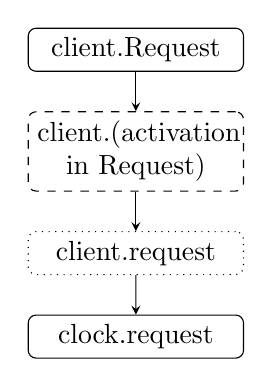
\begin{tikzpicture}[
    arrowstyle/.style={draw, -stealth},
    edge from parent/.style={draw, -stealth},
    reaction/.style={rectangle, draw, rounded corners=1mm, text width=2.5cm,
        text centered, anchor=north},
    activation/.style={rectangle, draw, rounded corners=1mm, dashed, text width=2.5cm,
        text centered, anchor=north},
    push/.style={rectangle, draw, rounded corners=1mm, dotted, text width=2.5cm,
        text centered, anchor=north},
    level 1/.style={sibling distance=7.0cm},
    level 2/.style={sibling distance=4.0cm},
    level 3/.style={sibling distance=3.0cm},
    level distance=0.5cm, growth parent anchor=south
]
\node (Action) [reaction] {client.Request}
  child {
    node (Activation01) [activation] {client.(activation in Request)}
    child {
      node (Push01) [push] {client.request}
      child {
        node (Reaction01) [reaction] {clock.request}
      }
    }
  }
;
\end{tikzpicture}
\endgroup
%%}%
\cprotect\caption{Transaction diagram for the \verb+client.Request+ action of the Clock System}
\label{request_transaction}
\end{figure}

\begin{figure}
\centering
%%\resizebox{\textwidth}{!}{%
\begingroup
\fontsize{10pt}{12pt}\selectfont
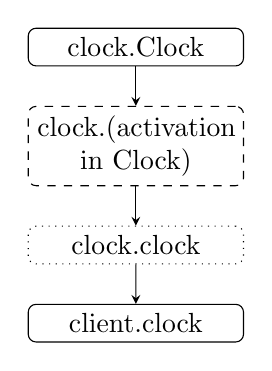
\begin{tikzpicture}[
    arrowstyle/.style={draw, -stealth},
    edge from parent/.style={draw, -stealth},
    reaction/.style={rectangle, draw, rounded corners=1mm, text width=2.5cm,
        text centered, anchor=north},
    activation/.style={rectangle, draw, rounded corners=1mm, dashed, text width=2.5cm,
        text centered, anchor=north},
    push/.style={rectangle, draw, rounded corners=1mm, dotted, text width=2.5cm,
        text centered, anchor=north},
    level 1/.style={sibling distance=7.0cm},
    level 2/.style={sibling distance=4.0cm},
    level 3/.style={sibling distance=3.0cm},
    level distance=0.5cm, growth parent anchor=south
]
\node (Action) [reaction] {clock.Clock}
  child {
    node (Activation01) [activation] {clock.(activation in Clock)}
    child {
      node (Push01) [push] {clock.clock}
      child {
        node (Reaction01) [reaction] {client.clock}
      }
    }
  }
;
\end{tikzpicture}
\endgroup
%%}%
\cprotect\caption{Transaction diagram for the \verb+clock.Clock+ action of the Clock System}
\label{clock_transaction}
\end{figure}

\section{Properties of Composition}
\label{propcomp}
In this section, we examine various features related to reactive components and composition.
Substitutional equivalence for reactive components is demonstrated by outlining a procedure for in-lining sub-components.
Hazards of composition, namely, non-deterministic state transitions resulting from conflicting and recursive composition, are identified and a means of detecting them is proposed.
The issue of decomposition is considered and \emph{pull ports} are introduced as a mechanism for decomposition.

\begin{figure}
\begin{verbatim}
component System {
  /* Substitution of clock component. */
  var int clock_counter (0)
  var bool clock_flag (false)
  push clock_clock(int t)

  reaction clock_request() clock_flag := true

  clock_Clock: clock_flag -> clock_flag := false activates clock_clock(clock_counter)

  clock_Tick: clock_counter := clock_counter + 1

  /* Substitution of client component. */
  var bool client_flag (false)
  push client_request()

  client_Request: !client_flag -> client_flag := true activates client_request()

  reaction client_clock(int t) client_flag := false || /* do something with t */

  bind {
    client_request -> clock_request
    clock_clock -> client_clock
  }
}
\end{verbatim}
\caption[Substitution of sub-components for the Clock System]{Substitution of state variables, ports, actions, and reactions for the sub-components of the System component of the Clock System}
\label{se1}
\end{figure}

\begin{figure}
\begin{verbatim}
component System {
  var int clock_counter (0)
  var bool clock_flag (false)
  var bool client_flag (false)
  push clock_clock(int t)
  push client_request()

  clock_Clock: clock_flag -> clock_flag, client_flag :=
    false, false activates clock_clock(clock_counter) ||
    /* do something with clock_counter */

  client_Request: !client_flag -> client_flag, clock_flag :=
    true, true activates client_request()

  clock_Tick: clock_counter := clock_counter + 1
}
\end{verbatim}
\caption[Simplification of expanded System component of the Clock System]{Simplifications of ports, bindings, and transitions in the expanded System component of the Clock System}
\label{se2}
\end{figure}

\subsection{Substitutional Equivalence}
\label{substitutional_equivalence}
For reactive components, substitutional equivalence means that a sub-component can be replaced with its definition and the result is a well-defined entity in the model.
To this end, a procedure for substituting the definition of a sub-component involves 1) renaming and adding all state variables, ports, actions, and reactions to the parent component and 2) simplifying bindings by substituting the transitions associated with a reaction into the action or reaction that activates the reaction in question.

To illustrate, Figure~\ref{se1} shows the result of substituting state variables, ports, actions, and reactions into the System component of Figure~\ref{system_component}.
Identifiers in the sub-components have been prefixed with the name of the sub-component instance to avoid name clashes.
For example, the \verb+request+ reaction in the \verb+clock+ sub-component has been renamed to \verb+clock_request+.
Figure~\ref{se2} shows the result of simplifying bindings and state transitions.
Note that the push ports have been retained for subsequent composition, i.e., the System component may be a component in a larger system.
The result is a reactive component whose ``size'' in terms of state variables, actions, and reactions is the sum of the sizes  of its constituent components.
Substituting the definition of the Clock component and Client components into the System component confirms the intuition that the flag variable in the client and flag variable in the clock are the same since 1) initially they have the same value and 2) they take on the same value in every state transition.

\subsection{Determinism and Composition}
\label{determinism}

\begin{figure}
\centering
%%\resizebox{\textwidth}{!}{%
\begingroup
\fontsize{10pt}{12pt}\selectfont
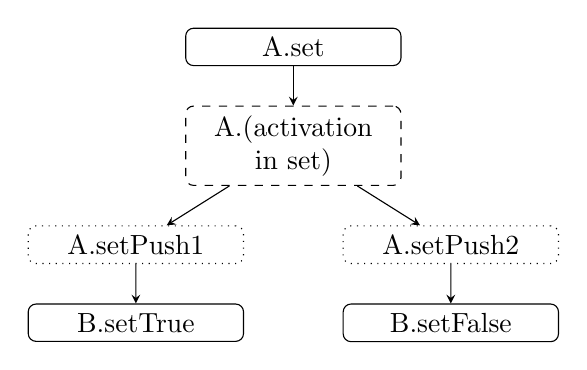
\begin{tikzpicture}[
    arrowstyle/.style={draw, -stealth},
    edge from parent/.style={draw, -stealth},
    reaction/.style={rectangle, draw, rounded corners=1mm, text width=2.5cm,
        text centered, anchor=north},
    activation/.style={rectangle, draw, rounded corners=1mm, dashed, text width=2.5cm,
        text centered, anchor=north},
    push/.style={rectangle, draw, rounded corners=1mm, dotted, text width=2.5cm,
        text centered, anchor=north},
    level 1/.style={sibling distance=7.0cm},
    level 2/.style={sibling distance=4.0cm},
    level 3/.style={sibling distance=3.0cm},
    level distance=0.5cm, growth parent anchor=south
]
\node (Action) [reaction] {A.set}
  child {
    node (Activation01) [activation] {A.(activation in set)}
    child {
      node (Push01) [push] {A.setPush1}
      child {
        node (Reaction01) [reaction] {B.setTrue}
      }
    }
    child {
      node (Push02) [push] {A.setPush2}
      child {
        node (Reaction02) [reaction] {B.setFalse}
      }
    }
  }
;
\end{tikzpicture}
\endgroup
%%}%
\caption{Transaction diagram for a non-deterministic transaction}
\label{ndt}
\end{figure}

The result of composing two well-defined reactive components may yield a system that is non-deterministic.
The two ``hazards'' that must be avoided are non-deterministic assignment to state variables and recursively activated reactions.
Non-deterministic assignment results when the next value for a state variable is not well defined due to the inclusion of two or more transitions in a transaction that operate on the state variable.
To illustrate, consider the transaction depicted in Figure~\ref{ndt}.
The set action of component A has a single activation that activates both the setPush1 and setPush2 push ports.
The setPush1 port is bound to the setTrue reaction of component B while the setPush2 port is bound to the setFalse reaction of the same component B.
Suppose that the setTrue reaction sets a flag to true while the setFalse reaction sets the same flag to false.
The transaction is non-deterministic because the value of the flag after the (A,set) transaction may either be true or false.
An offending pair of transitions may appear anywhere in a transaction graph given that arbitrary transaction graphs may be constructed through composition.
If the underlying language used to define transitions admits pointers, dynamic memory, if statements, and loops (i.e., is Turing-complete), then the problem of determining if two transitions operate on the same state variable is undecidable in general~\cite{Landi:1992:USA:161494.161501, Ramalingam:1994:UA:186025.186041}.
For a transaction graph $G$, instances $i_1$ and $i_2$, and actions/reactions $t_1$ and $t_2$, a necessary (but not sufficient) condition for non-deterministic assignment $\mathit{NDA}$ from composition is $\mathit{NDA}(G): \exists (i_1, t_1), (i_2, t_2) \in G.N, i_1 = i_2, t_1 \ne t_2$ which says that the transaction must contain two different transitions involving the same component instance.

A recursively activated transition occurs when the transaction graph has a cycle.
The execution of such a transaction may result in well-defined next values for all state variables assuming that 1)~the recursion is bounded and 2)~the parameters passed to every reaction result in identical computations.
A transaction may be analyzed like a traditional transformational program since it has finite input, a finite output, and should terminate.
The first problem, then, is a thinly disguised version of the halting problem since it asks if a computation (the transaction) expressed in a Turing-complete language terminates (has bounded recursion)~\cite{Turing01011937, davis1958computability}.
A bounded recursion means that the execution of the transaction will generate a bounded number of activations $A$.
For each activation $a \in A$, we must determine what state is updated by $a$.
If the language is Turing-complete, then this problem is undecidable in general~\cite{Landi:1992:USA:161494.161501, Ramalingam:1994:UA:186025.186041}.
For state variables that are updated by more than one activation, we must then show that each activation sets the state variable to the exact same next state.
If we treat each activation as a program, then we require a function that determines if two (arbitrary) programs compute the same function, which is again, undecidable in general~\cite{Rice:53}.

The difficulty of detecting composition that results in non-deterministic assignments suggests that these problems are best checked by a machine.
That is, an implementation of reactive components may prevent non-deterministic assignment by checking that $\mathit{NDA}(G)$ is false for all transaction graphs in the system.
Similarly, an implementation may check for recursive activation by checking for cycles in transaction graphs.
Both of these approaches are used by the implementation described in Section~\ref{sound_composition}.

\subsection{Decomposition, Getters, and Pull Ports}
\label{decomposition}
Substitutional equivalence implies that the process of substituting the definition of a sub-component into a parent component may be reversed and that sub-components may be ``factored out'' of an existing component, e.g., for reuse with other components.
%% One motivation for extracting sub-components is to support the software engineering practice of refactoring where common code is extracted so that it can be reused in various places.

Another motivation for decomposition is potentially increased performance through parallelism.
Recall that true concurrency in reactive components is modeled as the serial and non-deterministic execution of atomic actions.
Two transactions can be safely executed concurrently if it can be shown that the state variables involved in each transaction are disjoint.
As was previously mentioned, making this determination is undecidable for Turing-complete languages in the general case.
However, the problem becomes decidable if the component instance is used as a proxy for its constituent state variables.
Let $\mathit{rw}: t \to \{ \mathit{Read}, \mathit{Write} \}$ be a function that maps a transition to a value indicating that variables are read-only during the transition or written in some way.
Two instance/transition pairs are independent ($\mathit{indp}$) if either the instances are different or at most one of the transitions writes to the variables of the instance:
\begin{equation}
\mathit{indp}((i_1, t_1), (i_2, t_2)): i_1 \ne i_2 \lor \lnot (\mathit{rw}(t_1) = \mathit{Write} \land \mathit{rw}(t_2) = \mathit{Write})
\end{equation}
Two transaction graphs are independent if all of their nodes are independent $\mathit{indp}(G_1, G_2) = \forall (i_1, t_1) \in G_1.N, (i_2, t_2) \in G_2.N \; \mathit{indp}((i_1, t_1), (i_2, t_2))$.
The significance of the preceding analysis is that the determination about what actions can be executed concurrently becomes machine checkable due to the strong guarantee that state variables belonging to an instance can only be modified by the transitions of that instance.

To illustrate the mechanisms required for decomposition, we will factor out a Counter component from the Clock component of Figure~\ref{clock_component} and then rewrite the Clock component using the Counter component.
Upon inspection, the \verb+Tick+ action and \verb+request+ reaction can be executed concurrently since the state variables involved in each transition are disjoint.
Figure~\ref{counter_component} shows the Counter component which consists of a \verb+counter+ state variable.
The \verb+Tick+ action can be moved to the Counter component without complication.
The \verb+Clock+ action of the Clock component \emph{reads} the value of \verb+counter+ which suggests that a mechanism for accessing the state variables in a component is required.
Thus, we introduce the notion of a \emph{getter} method which can be called on a component to produce a value that may be derived from its state variables.
In the Counter component, the \verb+getCounter+ getter returns the current value of the counter.
A getter is not allowed to modify the state of a component and may only be invoked in the immutable phase.
These semantics preserve the strict separation of immutable phase and mutable phase.
When analyzing composition, a getter is treated like a transition that reads the state variable of the corresponding instance.
Figure~\ref{factored_clock_component} shows the Clock component rewritten to use a Counter sub-component and a getter.

\begin{figure}
\begin{verbatim}
component Counter {
  var int counter (0)

  Tick: counter := counter + 1

  getCounter() int {
    return counter
  }
}
\end{verbatim}
\caption{Definition of the Counter component of the Factored Clock System}
\label{counter_component}
\end{figure}

\begin{figure}
\begin{verbatim}
component Clock {
  var Counter c
  var bool flag (false)
  push clock(int t)

  reaction request() flag := true

  Clock: flag -> flag := false activates clock(c.getCounter())
}
\end{verbatim}
\caption{Definition of the Clock component of the Factored Clock System}
\label{factored_clock_component}
\end{figure}

The logic associated with the \verb+flag+ state variable represents a generic request-response protocol except for the call to \verb+c.getCounter()+.
To indirect the call to \verb+c.getCounter()+ we introduce the notion of a \emph{pull port}.
A pull port represents an external value dependency.
A component can demand a value from the pull port in the immutable phase.
Like push ports, pull ports have an active and passive side.
The active side represents the caller and the passive side represents the callee.
Getters are sufficient to realize the passive side of a pull port.
Every active pull port must be bound to exactly one passive pull port via composition.
Figure~\ref{request_response_component} shows a component that implements the request-response protocol using a pull port \verb+getValue+.
Figure~\ref{factored2_clock_component} shows the Clock component written in terms of the Counter and RequestResponse components.
An \verb+export+ directive allows reactions, getters, and ports in sub-components to be available in the interface of the encapsulating component.

\begin{figure}
\begin{verbatim}
component RequestResponse {
  var bool flag (false)
  pull getValue() int
  push response(int t)

  reaction request() flag := true

  Response: flag -> flag := false activates response(getValue())
}
\end{verbatim}
\caption{Definition of the RequestResponse component of the Factored Clock System}
\label{request_response_component}
\end{figure}

\begin{figure}
\begin{verbatim}
component Clock {
  var Counter c
  var RequestResponse rr
  push request()
  push clock(int t)

  bind {
    c.getCounter -> rr.getValue
  }

  export rr.request as request
  export rr.response as clock
}
\end{verbatim}
\caption{Definition of the Clock component of the Factored Clock System (fully-factored)}
\label{factored2_clock_component}
\end{figure}

Pull ports are subject to a hazard of composition similar to the recursive activation hazard of push ports.
A cycle in the graph of composed pull ports is equivalent to a recursively defined function.
The recursion may be bounded but this is undecidable in the general case.
Consequently, an implementation may reject recursively defined getters and pull ports.

\section{Summary}
In this chapter, we have presented the reactive component model for reactive programs.
A reactive component consists of a set of state variables and transitions that are private to the component.
The interface of a reactive component consists of push ports and reactions, which allow a component to trigger a transition in another component, and pull ports and getters, which allow a component to access the state of another component.
The external or visible behavior of a reactive component can be traced through its interface, specifically its push ports.
The internal details of a component can often be abstracted away to permit reasoning about the behavior of a composed system at various levels of detail.
Composition is achieved through recursive encapsulation (sub-components) and explicit port binding and satisfies the requirements for principled composition set forth in Section~\ref{challenges}.
As demonstrated in Section~\ref{substitutional_equivalence}, the definitions of sub-components can be substituted into the containing component resulting in an equivalent system (substitutional equivalence).
Similarly, sub-components may be ``factored out'' by using pull ports and getters to safely access the state of the sub-components.

The private nature of state variables and transitions causes properties established from the text of a component to be preserved through composition.
Composition links transitions to form an atomic transaction that allows the properties of one component to be related to another component.
When the sub-components of a component are protected from further composition, the properties derived from their interactions are preserved as the parent component is composed.
Property-preserving composition is essential for reasoning about systems in a hierarchical and/or modular fashion.

The result of composing reactive components is either well-defined due to the atomic nature of transactions or illegal due to the composition hazards of recursive transactions and non-deterministic state transitions.
Analysis of these hazards at the state variable level is impossible due to the undecidable nature of their sub-problems.
This suggests that implementations may restrict composition to prevent the conditions necessary for recursive transactions and non-deterministic state transitions.
The main concession is allowing a component instance to proxy for its state variables.
The problem of detecting recursive transactions, then, can be posed as the problem of detecting cycles in a directed graph.
Similarly, the problem of detecting potentially non-deterministic state transitions is reduced to a set membership problem.
Valid systems that fail the check for non-deterministic state transitions using component instance proxies can be refactored by decomposing  the offending components.

        }%

% State variables
\onslide<2>
\begin{tikzpicture}[overlay,remember picture]
  \pgftransformshift{\pgfpointanchor{current page}{center}}
  \node [draw, rectangle, minimum height=50, minimum width=60, red, very thick] at (.3,2.3) {};
\end{tikzpicture}

% Transitions
\onslide<3>
\begin{tikzpicture}[overlay,remember picture]
  \pgftransformshift{\pgfpointanchor{current page}{center}}
  \node [draw, rectangle, minimum height=30, minimum width=50, red, very thick] at (.2,.8) {};
  \node [draw, rectangle, minimum height=30, minimum width=50, red, very thick] at (.2,-.5) {};
\end{tikzpicture}

% Active Push Port
\onslide<4>
\begin{tikzpicture}[overlay,remember picture]
  \pgftransformshift{\pgfpointanchor{current page}{center}}
  \node [draw, rectangle, minimum height=20, minimum width=70, red, very thick] at (4.1,.85) {};
  \node [draw, rectangle, minimum height=20, minimum width=60, red, very thick, dashed] at (-3.6,.85) {};
\end{tikzpicture}

% Precondition
\onslide<5>
\begin{tikzpicture}[overlay,remember picture]
  \pgftransformshift{\pgfpointanchor{current page}{center}}
  \node [draw, rectangle, minimum height=25, minimum width=50, red, very thick] at (-1.5,-.7) {};
\end{tikzpicture}

% Action
\onslide<6>
\begin{tikzpicture}[overlay,remember picture]
  \pgftransformshift{\pgfpointanchor{current page}{center}}
  \node [draw, rectangle, minimum height=35, minimum width=100, red, very thick] at (-.6,-.7) {};
\end{tikzpicture}

% Reaction
\onslide<7>
\begin{tikzpicture}[overlay,remember picture]
  \pgftransformshift{\pgfpointanchor{current page}{center}}
  \node [draw, rectangle, minimum height=30, minimum width=170, red, very thick] at (-1.7,.8) {};
\end{tikzpicture}

% Active Pull Port
\onslide<8>
\begin{tikzpicture}[overlay,remember picture]
  \pgftransformshift{\pgfpointanchor{current page}{center}}
  \node [draw, rectangle, minimum height=20, minimum width=70, red, very thick, dashed] at (4.1,-1.6) {};
  \node [draw, rectangle, minimum height=20, minimum width=60, red, very thick] at (-3.6,-1.6) {};
\end{tikzpicture}

% Expression
\onslide<9>
\begin{tikzpicture}[overlay,remember picture]
  \pgftransformshift{\pgfpointanchor{current page}{center}}
  \node [red] at (2.4,-3.2) {interrogate state variables};
  \node [draw, rectangle, minimum height=15, minimum width=60, red, very thick] at (2.3,-2.3) {};
\end{tikzpicture}

% Getter
\onslide<10>
\begin{tikzpicture}[overlay,remember picture]
  \pgftransformshift{\pgfpointanchor{current page}{center}}
  \node [draw, rectangle, minimum height=40, minimum width=110, red, very thick] at (3.1,-1.9) {};
\end{tikzpicture}

\end{frame}

\begin{frame}{Transitions, Transactions, and Execution}

\begin{block}{Transitions}
  Conceptually, a \emph{transition} is an atomic parallel assignment statement:

  \hspace{4em} var1, var2, ... := expr1, expr2, ...

  \hspace{4em} \emph{Mutable Phase} := \emph{Immutable Phase}
\end{block}

\begin{block}{Transactions}
  A \emph{transaction} is a set of transitively linked transitions.
\end{block}

\begin{block}{(Logical) Execution}
  Repeatedly execute transactions (order is not determined).
\end{block}

\begin{block}{Fairness}
  All transactions are selected an infinite number of times.
\end{block}
\end{frame}

\begin{frame}{Clock System Example 
\includegraphics[height=12pt]{CLOCK01-300px.png}}

\vspace*{36pt}

\centering
\resizebox{\textwidth}{!}{%
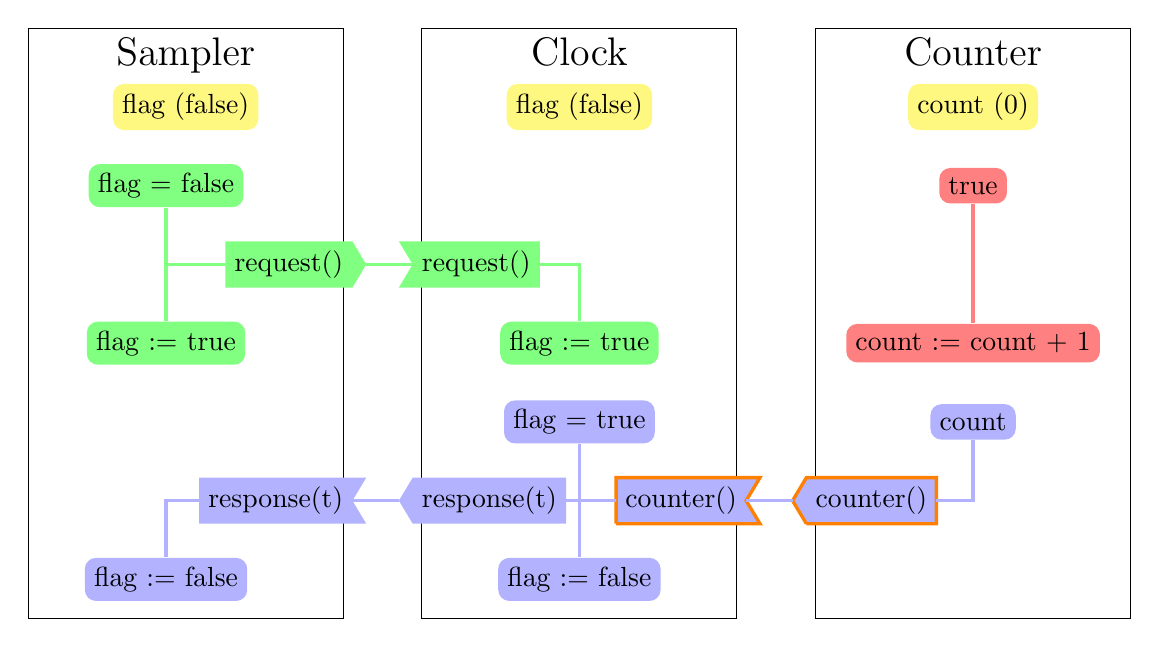
\begin{tikzpicture}
  [
    initial/.style={
      fill=yellow!50,
      rounded corners,
    },
    trans1/.style={
      fill=green!50,
    },
    trans1line/.style={
      draw=green!50,
    },
    trans2/.style={
      fill=blue!30,
    },
    trans2line/.style={
      draw=blue!30,
    },
    trans3/.style={
      fill=red!50,
    },
    trans3line/.style={
      draw=red!50,
    },
    line/.style={
      very thick
    },
    pre/.style={
      rectangle,
      rounded corners
    },
    post/.style={
      rectangle,
      rounded corners
    },
    pull/.style={
      draw=orange, very thick
    }
  ]
% Sampler
\draw (2,2.5) rectangle (6,10);
\node [below] at (4,10) {\Large Sampler};
\node [initial] at (4,9) {flag (false)};

\node (pre1)  [trans1, pre]            at (3.75,8) {flag = false};
\node (ex2a)  [trans1, shape=rightout] at (6,7)    {request()};
\node (post1) [trans1, post]           at (3.75,6) {flag := true};
\draw [trans1line, line] (pre1.south) |- (ex2a.west) -| (post1.north);

\node (ex3a)  [trans2, shape=rightin]  at (6,4)    {response(t)};
\node (post2) [trans2, post]           at (3.75,3) {flag := false};
\draw [trans2line, line] (ex3a.west) -| (post2.north);

% Clock
\draw (7,2.5) rectangle (11,10);
\node [below] at (9,10) {\Large Clock};
\node [initial] at (9,9) {flag (false)};

\node (ex2b)  [trans1, shape=leftin] at (7,7) {request()};
\node (post2) [trans1, post]         at (9,6) {flag := true};
\draw [trans1line, line] (ex2b.east) -| (post2.north);

\node (pre2)  [trans2, pre]           at (9,5)  {flag = true};
\node (ex3b)  [trans2, shape=leftout] at (7,4)  {response(t)};
\node (pull)  [trans2, shape=rightin, pull] at (11,4) {counter()};
\node (post3) [trans2, post]          at (9,3)  {flag := false};
\draw [trans2line, line] (pre2.south) |- (ex3b.east) -| (pull.west) -| (post3.north);

% Counter
\draw (12,2.5) rectangle (16,10);
\node [below] at (14,10) {\Large Counter};
\node [initial] at (14,9) {count (0)};

\node (pre4)  [trans3, pre]  at (14,8) {true};
\node (post4) [trans3, post] at (14,6) {count := count + 1};
\draw [trans3line, line] (pre4.south) -- (post4.north);

\node (pre3)   [trans2, pre]           at (14,5) {count};
\node (getter) [trans2, shape=leftout, pull] at (12,4) {counter()};
\draw [trans2line, line] (pre3.south) |- (getter.east);

\draw [trans1line, line] (ex2a.east) -- (ex2b.west);
\draw [trans2line, line] (ex3a.east) -- (ex3b.west);
\draw [trans2line, line] (pull.east) -- (getter.west);

\end{tikzpicture}
}%

% Variables
\onslide<2>
\begin{tikzpicture}[overlay,remember picture]
  \pgftransformshift{\pgfpointanchor{current page}{center}}
  \node [draw, rectangle, minimum height=20, minimum width=270, red, very thick] at (-.1,1.9) {};
\end{tikzpicture}

\onslide<3>
\begin{tikzpicture}[overlay,remember picture]
  \pgftransformshift{\pgfpointanchor{current page}{center}}
  \node [draw, rectangle, minimum height=60, minimum width=170, red, very thick] at (-2.05,.4) {};
\end{tikzpicture}

\onslide<4>
\begin{tikzpicture}[overlay,remember picture]
  \pgftransformshift{\pgfpointanchor{current page}{center}}
  \node [draw, rectangle, minimum height=60, minimum width=270, red, very thick] at (-.35,-1.9) {};
\end{tikzpicture}

\onslide<5>
\begin{tikzpicture}[overlay,remember picture]
  \pgftransformshift{\pgfpointanchor{current page}{center}}
  \node [draw, rectangle, minimum height=60, minimum width=80, red, very thick] at (3.75,.4) {};
\end{tikzpicture}


\end{frame}

\begin{frame}{Simplification of Clock System 
\includegraphics[height=12pt]{CLOCK01-300px.png}}

  \centering

  Reactive components allow principled composition.

\resizebox{\textwidth}{!}{%
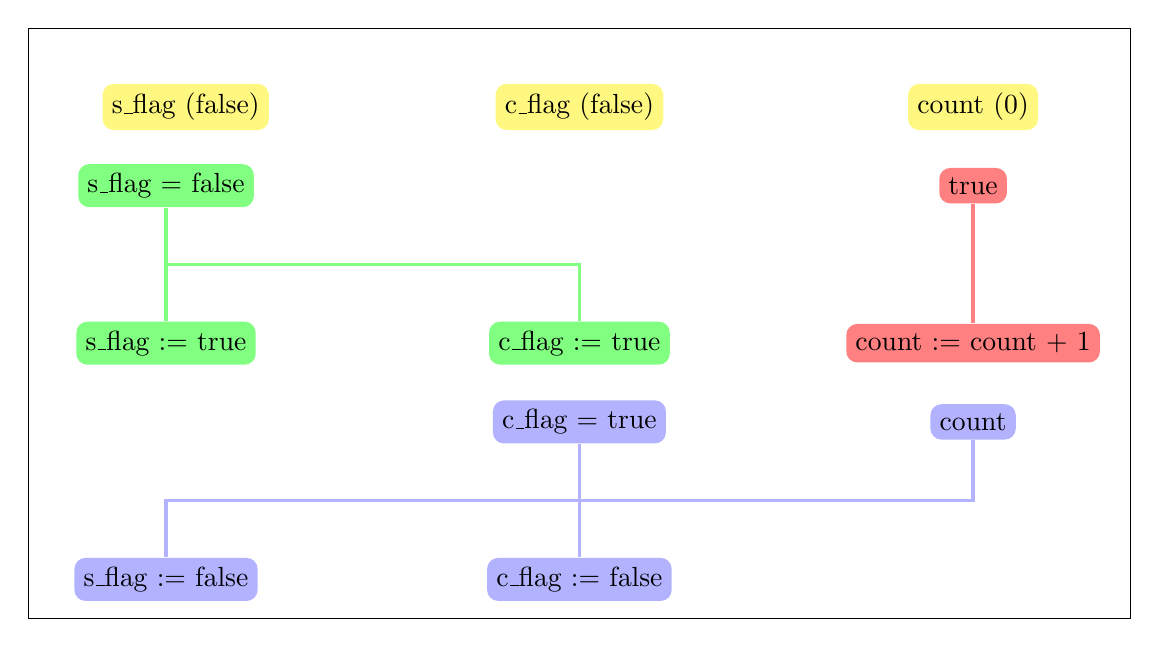
\begin{tikzpicture}
  [
    initial/.style={
      fill=yellow!50,
      rounded corners,
    },
    trans1/.style={
      fill=green!50,
    },
    trans1line/.style={
      draw=green!50,
    },
    trans2/.style={
      fill=blue!30,
    },
    trans2line/.style={
      draw=blue!30,
    },
    trans3/.style={
      fill=red!50,
    },
    trans3line/.style={
      draw=red!50,
    },
    line/.style={
      very thick
    },
    pre/.style={
      rectangle,
      rounded corners
    },
    post/.style={
      rectangle,
      rounded corners
    },
    pull/.style={
      draw=orange, very thick
    }
  ]
% Sampler
\draw (2,2.5) rectangle (16,10);
\node [initial] at (4,9) {s\_flag (false)};

\node (pre1)  [trans1, pre]            at (3.75,8) {s\_flag = false};
\node (post1) [trans1, post]           at (3.75,6) {s\_flag := true};
\draw [trans1line, line] (pre1.south) |- (6,7) -| (post1.north);

\node (post2) [trans2, post]           at (3.75,3) {s\_flag := false};
\draw [trans2line, line] (6,4) -| (post2.north);

% Clock
\node [initial] at (9,9) {c\_flag (false)};

\node (post2) [trans1, post]         at (9,6) {c\_flag := true};
\draw [trans1line, line] (7,7) -| (post2.north);

\node (pre2)  [trans2, pre]           at (9,5)  {c\_flag = true};
\node (post3) [trans2, post]          at (9,3)  {c\_flag := false};
\draw [trans2line, line] (pre2.south) |- (7,4) -| (11,4) -| (post3.north);

% Counter
\node [initial] at (14,9) {count (0)};

\node (pre4)  [trans3, pre]  at (14,8) {true};
\node (post4) [trans3, post] at (14,6) {count := count + 1};
\draw [trans3line, line] (pre4.south) -- (post4.north);

\node (pre3)   [trans2, pre]           at (14,5) {count};
\draw [trans2line, line] (pre3.south) |- (12,4);

\draw [trans1line, line] (6,7) -- (7,7);
\draw [trans2line, line] (6,4) -- (7,4);
\draw [trans2line, line] (11,4) -- (12,4);

\end{tikzpicture}
}%

\end{frame}

\begin{frame}{Platform Requirements}
  \begin{center}
  \begin{tikzpicture}
    [
      ampersand replacement=\&,
      node distance=5cm,
      node/.style={
        rectangle,
        draw,
        rounded corners,
        minimum height=3em,
        text width=2cm,
        text centered,
        very thick
      },
      line/.style = {
        >=stealth,
        ->,
        very thick,
      }
    ]

    \matrix [row sep=.25cm, column sep=1cm] {
      \node (m) [node] {Model}; \&
      \node (p) [node] {Platform}; \&
      \node (s) [node] {Systems}; \\
    };

    \node at ($(m.south east)!.5!(p.south west)$) {
\includegraphics[height=.75cm]{thumbs.png}};
    \node at ($(p.south east)!.5!(s.south west)$) {
\includegraphics[height=.75cm]{thumbs.png}};

    \draw[line] ($(m.south east)!.66!(m.north east)$) -- ($(p.south west)!.66!(p.north west)$);
    \draw[line] ($(p.south east)!.66!(p.north east)$) -- ($(s.south west)!.66!(s.north west)$);
    \draw[line] ($(s.south west)!.33!(s.north west)$) -- ($(p.south east)!.33!(p.north east)$);
    \draw[line] ($(p.south west)!.33!(p.north west)$) -- ($(m.south east)!.33!(m.north east)$);
  \end{tikzpicture}
  \end{center}

  \vspace*{-20pt}

  \begin{center}
  \begin{columns}
    \begin{column}{.25\textwidth}
      \center
      
\includegraphics[width=3cm]{mind_the_gap_edit.png}
    \end{column}
    \begin{column}{.75\textwidth}
      \center
      \begin{itemize}
      \item Strict enforcement of the model
      \item Reference semantics and linked data structures
      \item Efficient inter-component communication
      \end{itemize}
    \end{column}
  \end{columns}
  \end{center}

  \vspace*{-20pt}

  \begin{columns}
    \begin{column}{.5\textwidth}
      \begin{itemize}
      \item \rcgo{} is based on \emph{Go} 
\includegraphics[height=32pt]{gopher.png}
        \begin{itemize}
        \item Go is like C with methods, interfaces, and garbage collection
        \end{itemize}
      \item rc\textsubscript{java} would be different
      \end{itemize}
    \end{column}
    \begin{column}{.5\textwidth}
      \fbox{
        \parbox{\linewidth}{\raggedright
          \emph{Static System Assumption}:\\Number and configuration of components is fixed.
        }
      }
    \end{column}
  \end{columns}


\end{frame}

\begin{frame}{Model $\to$ Language}
  \centering

  \resizebox{\textwidth}{!}{%
    \chapter{Reactive Component Model}
\label{model}

In this chapter, we present a new model for composing and decomposing reactive programs via \emph{reactive components}.
The model is biased toward practical software development even as it enforces properties based in formal methods.
Consequently, the model favors utility, practicality, flexibility, and ease of implementation.
Unlike UNITY in which composition is not property-preserving, the composition of reactive components is property-preserving which facilitates hierarchical and modular reasoning.
Unlike I/O Automata in which transitions have limited depth, a transition among reactive components may access and cascade to an arbitrary number of other components, which permits decomposition to an arbitrary depth and degree.

%% \paragraph{Formal models and software engineering.}
%% I claim that most of the software that is ``put into production'' will never be proved formally correct.
%% This is a function of economics since modeling and constructing proofs is a labor-intensive process that can only be justified for safety or mission critical software.
%% However, I would argue that the development and application of formal models are critical to software engineering.
%% To illustrate, consider \emph{structured programming}~\cite{dahl1972structured}.
%% Structured programming assumes an abstract machine that executes programs that are restricted to a small set of well-defined control structures and assignment statements.
%% A program written in this form can be reasoned about directly from the text by formulating a Hoare-triple for each statement.
%% Structured programming opened the door for \emph{structured programming languages} which are also based on well-defined control structures and evaluation semantics.
%% Thus, while very few programmers will prove their structured programs correct, all of them informally use structured programming when they are fixing a bug revealed by a unit test or analyzing a core dump in a debugger.
%% Structured programming languages reduced the accidental complexity associated with writing the same program in assembly language.

%% The realm of reactive programs is waiting for a similar reduction in accidental complexity.
%% Taking a hint from structured programming, I believe two things are required.
%% First, we must write reactive programs against an easy-to-reason-about abstract machine instead of low-level interfaces like atomic instructions and thread libraries.
%% Second, we must restrict the form of reactive programs so that they can be reasoned about from the text.
%% I hope the proposed model of reactive systems is a step toward toward this goal.

\section{Features of the Model}

%% left active pull port
%% x, y, width, height, label
\def\lapull[#1,#2,#3,#4,#5,#6]#7{
  \draw [fill=lightgray] (#1,#2) -- ++(${#4*.5}*(-1,0) + {#4*.5}*(0,-1)$) -- ++($#3*(1,0)$) -- ++($#4*(0,1)$) -- ++($#3*(-1,0)$) -- cycle;
  \node (#5) at (#1,#2) {};
  \node (#6) at ($(#1,#2) + {#3 - .5 * #4}*(1,0)$) {};
  \node [right, align=left] at (#1,#2) {#7};
}

%% left active push port
%% x, y, width, height, label
\def\lapush[#1,#2,#3,#4,#5,#6]#7{
  \draw [fill=white] ($(#1,#2) + {#4*.5}*(-1,0)$) -- ++(${#4*.5}*(1,0) + {#4*.5}*(0,-1)$) -- ++($#3*(1,0)$) -- ++($#4*(0,1)$) -- ++($#3*(-1,0)$) -- cycle;
  \node (#5) at ($(#1,#2) - .5*#4*(1,0)$) {};
  \node (#6) at ($(#1,#2) + {#3}*(1,0)$) {};
  \node [right, align=left] at (#1,#2) {#7};
}

%% left passive pull port
%% x, y, width, height, label
\def\lppull[#1,#2,#3,#4,#5,#6]#7{
  \draw [fill=lightgray] ($(#1,#2) + {#4*.5}*(-1,0)$) -- ++(${#4*.5}*(1,0) + {#4*.5}*(0,-1)$) -- ++($#3*(1,0)$) -- ++($#4*(0,1)$) -- ++($#3*(-1,0)$) -- cycle;
  \node (#5) at ($(#1,#2) - .5*#4*(1,0)$) {};
  \node (#6) at ($(#1,#2) + {#3}*(1,0)$) {};
  \node [right, align=left] at (#1,#2) {#7};
}

%% left passive push port
%% x, y, width, height, label
\def\lppush[#1,#2,#3,#4,#5,#6]#7{
  \draw [fill=white] (#1,#2) -- ++(${#4*.5}*(-1,0) + {#4*.5}*(0,-1)$) -- ++($#3*(1,0)$) -- ++($#4*(0,1)$) -- ++($#3*(-1,0)$) -- cycle;
  \node (#5) at (#1,#2) {};
  \node (#6) at ($(#1,#2) + {#3 - .5*#4}*(1,0)$) {};
  \node [right, align=left] at (#1,#2) {#7};
}

%% right passive pull port
%% x, y, width, height, label
\def\rppull[#1,#2,#3,#4,#5,#6]#7{
  \draw [fill=lightgray] ($(#1,#2) + {#4*.5}*(1,0)$) -- ++(${#4*.5}*(-1,0) + {#4*.5}*(0,-1)$) -- ++($#3*(-1,0)$) -- ++($#4*(0,1)$) -- ++($#3*(1,0)$) -- cycle;
  \node (#5) at ($(#1,#2) + {#4*.5}*(1,0)$) {};
  \node (#6) at ($(#1,#2) + {#3}*(-1,0)$) {};
  \node [left] at (#1,#2) {#7};
}

%% right active push port
%% x, y, width, height, label
\def\rapush[#1,#2,#3,#4,#5,#6]#7{
  \draw [fill=white] ($(#1,#2) + {#4*.5}*(1,0)$) -- ++(${#4*.5}*(-1,0) + {#4*.5}*(0,-1)$) -- ++($#3*(-1,0)$) -- ++($#4*(0,1)$) -- ++($#3*(1,0)$) -- cycle;
  \node (#5) at ($(#1,#2) + {#4*.5}*(1,0)$) {};
  \node (#6) at ($(#1,#2) + {#3}*(-1,0)$) {};
  \node [left] at (#1,#2) {#7};
}

%% right passive push port
%% x, y, width, height, label
\def\rppush[#1,#2,#3,#4,#5,#6]#7{
  \draw [fill=white] (#1,#2) -- ++(${#4*.5}*(1,0) + {#4*.5}*(0,-1)$) -- ++($#3*(-1,0)$) -- ++($#4*(0,1)$) -- ++($#3*(1,0)$) -- cycle;
  \node (#5) at (#1,#2) {};
  \node (#6) at ($(#1,#2) + {#3 - .5*#4}*(-1,0)$) {};
  \node [left] at (#1,#2) {#7};
}

%% right active pull port
%% x, y, width, height, label
\def\rapull[#1,#2,#3,#4,#5,#6]#7{
  \draw [fill=lightgray] (#1,#2) -- ++(${#4*.5}*(1,0) + {#4*.5}*(0,-1)$) -- ++($#3*(-1,0)$) -- ++($#4*(0,1)$) -- ++($#3*(1,0)$) -- cycle;
  \node (#5) at (#1,#2) {};
  \node (#6) at ($(#1,#2) + {#3 - .5*#4}*(-1,0)$) {};
  \node [left] at (#1,#2) {#7};
}

\begin{figure}[H]
\centering
\resizebox{\textwidth}{!}{%
\begingroup
\fontsize{10pt}{12pt}\selectfont
\begin{tikzpicture}
[
arrowstyle/.style={
  decoration={markings,mark=at position 1 with {\arrow[scale=2,]{stealth}}},
  postaction={decorate},
  shorten >=0.4pt
}
]

%% component boundary
\draw (0,0) rectangle (10,8.25);
%% active pull ports
\lapull[0,1.5,1,.5,apullex1,apullin1]{}
\node[align=center] at (-1,1.5) {active\\pull port};
\lapull[0,.5,1,.5,apullex2,apullin2]{}
%% passive pull ports
\rppull[10,1.5,1,.5,ppullex1,ppullin1]{}
\node[align=center] at (11,1.5) {passive\\pull port};
\rppull[10,.5,1,.5,ppullex2,ppullin2]{}
\draw[thick] (apullin2.center) -- (ppullin2.center);
%% actions and rections
\node[draw, diamond, minimum height=15, minimum width=20] (pre) at (2.5,3) {};
\node at (2.5,2.5) {precondition};
\node[draw, minimum height=15, minimum width=50, rounded corners=5] (trans1) at (5,3) {};
\draw[dashed] (3.5,3) ellipse (3 and 1);
\node at (3.5,3.5) {\textbf{\emph{action}}};
\node[draw, minimum height=15, minimum width=50, rounded corners=5] (trans2) at (5,5) {};
\node at (5,4.5) {transition};
\draw[thick,arrowstyle] (pre) -- (trans1);
\draw[thick] (apullin1.center) -| (trans1) node[pos=.5,right] {\textbf{call}};
%% active push ports
\rapush[10,3,1,.5,apushex1,apushin1]{}
\rapush[10,4,1,.5,apushex2,apushin2]{}
\rapush[10,5,1,.5,apushex3,apushin3]{}
\node[align=center] at (11.1,5) {active\\push port};
\draw[thick,dashed,arrowstyle] (trans1) -- (apushin1.center);
\draw[thick,dashed,arrowstyle] (trans1) -- (apushin2.center);
\node at(7.5,4) {\textbf{activate}};
\draw[thick,dashed,arrowstyle] (trans2) -- (apushin2.center);
\draw[thick,dashed,arrowstyle] (trans2) -- (apushin3.center);
%% passive push ports
\lppush[0,5,1,.5,ppushex1,ppushin1]{}
\draw[thick,arrowstyle] (ppushin1.center) -- (trans2);
\node[align=center] at (-1.1,5) {passive\\push port};
\draw[dashed] (2,5) ellipse (5 and 1);
\node at (2,5.5) {\textbf{\emph{reaction}}};
\node[draw, cylinder, shape border rotate=90, minimum height=40, minimum width=40] (sv1) at (5,7.25) {};
\node[align=center] at (5,6.25) {state variables};
\end{tikzpicture}
\endgroup
}%
\caption{Features of a reactive component\label{reactive_component}}
\end{figure}

Figure~\ref{reactive_component} shows the major features of a reactive component.
As in other state-based formal models like UNITY~\cite{chandy1989parallel} and I/O Automata~\cite{nancy1996distributed}, the core of a reactive component in this model is a set of \emph{state variables} and a set of atomic \emph{transitions} that manipulate those state variables.
When reasoning about a system, behavior is expressed as propositions over the state variables where the propositions are derived from the transitions.

%% The contribution that this work makes to existing state-based formal models of reactive systems is a combination of interface elements and composition semantics that allow reactive programs to be composed in a principled way.

The reactive component model defines interface elements and composition semantics that allow reactive programs to be composed in a principled way.
For example, an \emph{active push port} allows a transition in one component to be linked to a transition in another component such that the resulting combined transition is atomic.
Active push ports allow reactive components to publicize their behavior.
An active push port may be \emph{bound} to and conditionally \emph{activate} zero or more \emph{passive push ports}.
A passive push port names the corresponding transition that will be executed when the passive push port is activated.
This combination of passive push port and transition is called a \emph{reaction} because it reacts to a transition in another component.

The atomic linkage of a transition in one component to a transition in another component through the push port mechanism allows the properties of each component to be related to one another and more complex systems to be constructed by composing simpler systems.
Transitions that are not executed via a passive push port are executed by the scheduler.
A transition of this kind may be governed by a Boolean expression called a \emph{precondition}.
The combination of a precondition and transition is called an \emph{action} because it is a voluntary transition under the control of the containing component.

An \emph{active pull port} represents an immutable external data dependency.
The component may \emph{call} an active pull port to yield a value required in a transition.
Active pull ports must be bound to a \emph{passive pull port} which resembles a function returning a value, e.g., a getter or a predicate.
Where push ports allow components to publicize their behavior, pull ports allow components to safely publicize their internal state for use by other components.

Composition in the reactive component model has two main features.
The first is recursive encapsulation where a state variable in one component may represent an instance of another reactive component.
The second is the ability to bind push ports and pull ports through an \emph{explicit} set of \emph{bindings}.
The decision to use an explicit set of bindings (as opposed to implicit named-based matching) is more in keeping with the goals and techniques of practical software development, since it facilitates the use of software developed under different naming conventions, i.e., third-party software.
A third minor feature called \emph{exporting} is the ability of an encapsulating component to adopt interface elements of its sub-components without defining complimentary ports and transitions that do nothing but forward an activation or call.
The ability to publicize behavior and state and the ability to assemble well-defined behavior from existing behaviors in a straight-forward and flexible way are thus defining characteristics of the reactive component model.

\begin{figure}
\centering
\resizebox{\textwidth}{!}{%
\begingroup
\fontsize{10pt}{12pt}\selectfont
\begin{tikzpicture}
\draw (0,6.5) rectangle (5,10);
\node[below] at (2.5,10) {Web Server};
\rapull[5,9,3.4,.5,ex1a,ignore]{verify(HttpHeader)};
\rapush[5,8,3.6,.5,ex2a,ignore]{request(HttpRequest)};
\rppush[5,7,4.2,.5,ex3a,ignore]{respond(HttpResponse)};

\draw(6,2.5) rectangle (11,10);
\node[below] at (8.5,10) {Application Logic};
\lppull[6,9,3.4,.5,ex1b,ignore]{verify(HttpHeader)};
\lppush[6,8,3.8,.5,ex2b,ignore]{request(HttpRequest)};
\lapush[6,7,3.9,.5,ex3b,ignore]{respond(HttpResponse)};

\rapush[11,6,3.5,.5,ex4a,ignore]{request(DBRequest)};
\rppush[11,5,4.1,.5,ex5a,ignore]{respond(DBResponse)};

\rapush[11,3,2.4,.5,ex6a,ignore]{log(Message)};

\draw (12,4.5) rectangle (17,7);
\node[below] at (14.5,7) {Database};
\lppush[12,6,3.7,.5,ex4b,ignore]{request(DBRequest)};
\lapush[12,5,3.8,.5,ex5b,ignore]{respond(DBResponse)};

\draw (12,2.5) rectangle (17,4);
\node[below] at (14.5,4) {Logging Service};
\lppush[12,3,2.5,.5,ex6b,ignore]{log(Message)};

\draw (ex1a.center) -- (ex1b.center);
\draw (ex2a.center) -- (ex2b.center);
\draw (ex3a.center) -- (ex3b.center);
\draw (ex4a.center) -- (ex4b.center);
\draw (ex5a.center) -- (ex5b.center);
\draw (ex6a.center) -- (ex6b.center);

\end{tikzpicture}
\endgroup
}%
\caption{Diagram of a web application built using reactive components\label{web_server}}
\end{figure}

To demonstrate the utility of component interfaces and explicit support for property-preserving composition, we now present an illustrative design for a web application using reactive components, as is shown in Figure~\ref{web_server}.
The web application consists of five reactive components.
The first is an unnamed top-level component representing the complete application.
This component has four sub-components representing a web server, the application logic, a database, and a logging service.
The ports of the application logic component have been bound to the corresponding ports in the web server, database, and logging service components.
The interface of a component, which consists of its ports, provides insight into the behavior of the component.
For example, based on the interface of the web server component we may expect it to 1)~verify incoming HTTP requests\footnote{A production web server may verify that the requested HTTP method can be applied to the given URI, that content length limits are respected, that content types are supported, etc.}, 2)~pass on valid HTTP requests to the application, and 3)~accept HTTP responses from the application.

Figure~\ref{web_server} also demonstrates how reactive programs can be constructed by composing reactive components, so that a developer may focus on the application logic and use existing components for the web server, database, and logging service.
Furthermore, one can imagine developing three stateless components surrounding the application logic that do nothing but translate messages between application specific message types and the generic types required by the web server, database, and logging service.
The application logic, then, is completely isolated from the surrounding libraries and may be tested by providing mock components for the web server, database, and logging service.
The application logic itself has a well-defined interface and could be reused, say, by implementing a graphical front-end to drive the application instead of a web service.

\subsection{State Variables}
Part of the internal core of a reactive component is a set of state variables, which are the subject of the propositions that demonstrate the behavior of the system.
The state variables are manipulated by the assignment statements that constitute the transitions.
As in other formal models, the types of the state variables may be selected to make writing proofs easier.
%% That is, the state variables have mathematically friendly types like integers, sets, and lists.
However, implementations of the reactive component model must provide a concrete type system that allows the state variables to be realized on a given machine.
For example, the \rcgo{} language for reactive components presented in Chapter~\ref{language} of this dissertation uses the type system of Go to define the types of state variables.
The type of a state variable also may be a reactive component type, which facilitates recursive encapsulation.
For modeling purposes, state variables typically have \emph{value semantics} to avoid reasoning about references and aliasing.
However, and as a practical concession, we will introduce pointers for building arbitrary linked data structures (since we advocate an imperative state-based implementation) and discuss issues raised by introducing pointers into the reactive component model in Chapter~\ref{language}.

\subsection{Atomic State Transitions}
The rest of the internal core of a reactive component is a set of atomic state transitions that manipulate the state variables.
A precise definition of the atomicity of state transitions will be deferred to the subsequent sections on composition (Section~\ref{composition}) and execution (Section~\ref{execution}).
State variables and state transitions are private, meaning that transitions can only refer to the state variables of the associated reactive component and a transition in one reactive component can only be linked to a transition in another component through the composition mechanisms.
Thus, all initialization and updates to state variables can be determined by examining the transitions of the corresponding component.
The encapsulation of state variables contribute to composition being \emph{compositional}.
All properties established from the transitions of a component will continue to hold as the component participates in composition since the set of transitions that affect the state variables is fixed.
State transitions must be deterministic meaning that the next value of every state variable is uniquely and well defined.
State transitions defined by a sequence of simple assignments are implicitly deterministic.
However, special care must be take to ensure that state transitions are deterministic when described using parallel assignment statements as the same variable may appear on the left-hand-side and be assigned two different values~\cite{chandy1989parallel}.
As described in Sections~\ref{composition} and \ref{execution}, composition links transitions using parallel assignment which creates an opportunity for non-deterministic state transitions.
The problem of non-deterministic state transitions arising from composition is explored in Section~\ref{propcomp}.

The reactive component model presented in this chapter does not prescribe a specific language for encoding state transitions.
The language used depends on the goals and tastes of the one developing or analyzing the model.
For example, expressing transitions using the programming language of UNITY~\cite{chandy1989parallel} may allow the modeler to extract proofs from the text, a major goal of UNITY.
The approach used by I/O Automata~\cite{nancy1996distributed} is to specify the condition established by each transition.
As with state variables, we present a language that uses the statements and expressions of the Go programming language to encode state transitions in Chapter~\ref{language}.
This furthers our goal of making reactive components approachable by a general software engineering audience.
%% from Dr. Gill
%% which aims to allow models to be incorporated directly into standard software environments.
%% This isn't accurate.  Compatibility with existing software is not the goal nor should it be a goal as existing software is based on threads which cannot reasonably be integrated with reactive components.

\subsection{Actions, Reactions, Push Ports, Bindings, and Composition}
\label{composition}
A state transition is either part of an action or a reaction.
An \emph{action} is a state transition whose execution is under the control of the component to which it belongs.
The action is guarded by a \emph{precondition} that is guaranteed to be true the instant before the action is executed.
The precondition is a Boolean expression that determines if the action is \emph{enabled} or \emph{disabled}.
If the precondition is absent, it is assumed to be true.

A \emph{reaction} is a state transition whose execution is under the control of another action or reaction.
Thus, we require a mechanism for linking a reaction to an action or another reaction.
To do this, we introduce the notion of a \emph{push port}.
A push port is a typed interaction point consisting of an active side that conditionally \emph{activates} the port and provides arguments to the port, and a passive side that \emph{reacts} to the port and may access the arguments provided by the active side.
A reaction, therefore, is the combination of a passive push port and a state transition.

A \emph{binding} is a declaration that associates an active push port in one component with a reaction in another component.
The transition associated with the reaction is executed atomically with the transition that activates the active push port.
Composition in the reactive component model is achieved by declaring sub-components (recursive encapsulation) and linking transitions via binding.

\subsection{Transactions}

A \emph{transaction} is a compound and concrete state transition formed by expanding the activations in an instance/action pair, subject to the bindings in a system.
The instance and action that define a transaction are called the \emph{root} of the transaction.
A transaction is enabled/disabled if its root action is enabled/disabled.
Given the root instance and action, we may enumerate the active push ports that may be activated by the transition of the action.
Note that the activation of a push port is conditional, being under the control of the transition.
The push ports, in turn, activate reactions in particular component instances.
The transitions associated with the reactions may activate other push ports and so on.
This analysis can be repeated to discover all of the reactions that are linked to the root action.
The result is a \emph{transaction graph} which is a directed acyclic graph $G = (N,E)$.
Each node $n \in N$ is a pair $(i, x)$ where $i$ is a component instance and $x$ is either an action, reaction, activation, or push port.
Each edge $e \in E$ corresponds to a causal relationship between an action/reaction and an activation, an activation and a push port, or a push port and a reaction.
The edges between actions/reactions and activations indicate that the action/reaction \emph{may} execute the activation, as they may be conditionally executed.
The edges between activations and push ports and between push ports and reactions indicate that the implied push port or reaction \emph{will} be executed if the upstream activation is executed.

\subsection{Execution}
\label{execution}
We adopt the common practice of modeling concurrency with non-deterministically executed atomic actions as is done in UNITY~\cite{chandy1989parallel}, I/O Automata~\cite{nancy1996distributed}, and the Actor Model~\cite{agha1985actors}.
The execution of transactions is performed by a \emph{scheduler}.
The scheduler executes one transaction at a time, thus, each transaction is \emph{atomic} with respect to all other transactions.
A transaction is \emph{enabled} if its precondition is true.
When executing a transaction, the scheduler first evaluates the precondition and then executes the body of the transaction if the transaction is enabled.
Thus, executing an enabled transaction \emph{may} result in a state change while executing a disabled transaction \emph{never} causes a state change.
The scheduler is \emph{fair} meaning that each transaction is executed an infinite number of times.
The system may reach a \emph{fixed point} where all transactions are disabled.
The order in which transactions are executed is not determined, thus, execution is \emph{non-deterministic}.

We divide a state transition into two phases called the \emph{immutable phase} and the \emph{mutable phase}.
Logically, a transition assigns values to a set of state variables.
This can be modeled as a parallel assignment statement with a left-hand side (LHS) consisting of a list of state variables and a right-hand side (RHS) consisting of a list of expressions that provide the next value for each corresponding state variable.
The immutable phase corresponds to the computation of the RHS in a state transition.
The mutable phase corresponds to the update of the values on the LHS with the values on the RHS.
When transitions are linked with composition, we must relate the mutable and immutable phase in one state transition to the mutable and immutable phases of the other transitions in the transaction.
Let $A$ be a transition (action) and $R$ be a transition (reaction) that is activated by $A$.
Let $A_I$ be the immutable phase of $A$, $A_M$ be the mutable phase of $A$, $R_I$ be the immutable phase of $R$, and $R_M$ be the mutable phase of $R$.
For the sake of argument, assume that $A_I$ reads variables that are written in $R_M$ and that $R_I$ reads variables that are written in $A_M$.
We require that $A_I$ be evaluated before $A_M$, $R_I$ be evaluated before $R_M$, and $A_I$ be evaluated before $R_I$ since activation is conditional.
This leaves three possible sequences:
\begin{itemize}
\item $A_I A_M R_I R_M$.  In this sequence, a variable is first updated in $A_M$ and then the updated value is read in $R_I$.  The issue with this interpretation is that it does not compose well.  Ideally, we would like to be able to rewrite the transition as a single transition consisting of a single immutable phase and mutable phase.
\item $A_I R_I A_M R_M$ and $A_I R_I R_M A_M$.  These sequences resolve the issue with the first sequence by providing a clear immutable phase ($A_I R_I$) and mutable phase ($A_M R_M$ and $R_M A_M$).
\end{itemize}
Thus, with respect to transactions, all immutable phases (which includes all push port activations) are performed before all mutable phases.

\section{Example:  Clock System}
To illustrate the behavior of reactive components under this model, we rewrite the \emph{Clock automaton} example in \cite{nancy1996distributed} using reactive components.
The Clock automaton consists of a free-running counter and flag used to implement a request-response protocol.
Our Clock component is defined in Figure~\ref{clock_component}.
The state variables are identified with \verb+var+ and their initial values are provided.
The component contains a reaction named \verb+request+ for receiving requests to sample the current value of the counter.
The component also contains an active push port named \verb+clock+ for communicating the sampled value of the counter.
The \verb+Clock+ action is conditioned on the flag variable (which indicates that a request has been made) which when it executes resets the flag and communicates the value of \verb+counter+ by activating the \verb+clock+ port.
The \verb+Tick+ action increments the free-running counter.
The absence of a precondition means this action is always enabled.
A simple client for the Clock component that perpetually requests the current count is shown in Figure~\ref{client_component}.

\begin{figure}
\begin{verbatim}
component Clock {
  var int counter (0)
  var bool flag (false)
  push clock(int t)

  reaction request() flag := true

  Clock: flag -> flag := false activates clock(counter)

  Tick: counter := counter + 1
}
\end{verbatim}
\caption{Definition of the Clock component of the Clock System}
\label{clock_component}
\end{figure}

\begin{figure}
\begin{verbatim}
component Client {
  var bool flag (false)
  push request()

  Request: !flag -> flag := true activates request()

  reaction clock(int t) flag := false || /* do something with t */
}
\end{verbatim}
\caption{Definition of the Client of the Clock System}
\label{client_component}
\end{figure}

In isolation, a Clock component will increment its counter forever and a Client component will make a request and then stop.
In order to make the two components work together, we must compose them.
Figure~\ref{system_component} shows a System component that instantiates a Clock component and a Client component and binds the corresponding push ports in each instance.
In the composed system, the client's \verb+Request+ action will be executed activating the \verb+request+ port which in turn causes the \verb+request+ reaction in the clock to be executed.
Figure~\ref{request_transaction} shows the transaction graph for the \verb+Request+ action.
Eventually, the clock's \verb+Response+ action will be executed activating the \verb+clock+ port which in turn causes the \verb+clock+ reaction in the client to be executed with the current value of the clock's counter.
Figure~\ref{clock_transaction} shows the transaction graph for the \verb+Clock+ action.
In between these actions, the \verb+Tick+ action of the clock is incrementing the counter.

\begin{figure}
\begin{verbatim}
component System {
  var Clock clock
  var Client client

  bind {
    client.request -> clock.request
    clock.clock -> client.clock
  }
}
\end{verbatim}
\caption{Definition of the System component of the Clock System}
\label{system_component}
\end{figure}

\begin{figure}
\centering
%%\resizebox{\textwidth}{!}{%
\begingroup
\fontsize{10pt}{12pt}\selectfont
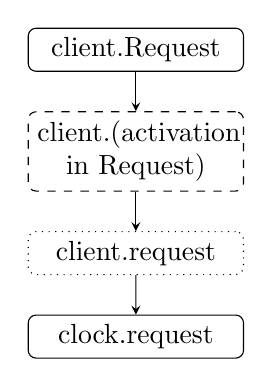
\begin{tikzpicture}[
    arrowstyle/.style={draw, -stealth},
    edge from parent/.style={draw, -stealth},
    reaction/.style={rectangle, draw, rounded corners=1mm, text width=2.5cm,
        text centered, anchor=north},
    activation/.style={rectangle, draw, rounded corners=1mm, dashed, text width=2.5cm,
        text centered, anchor=north},
    push/.style={rectangle, draw, rounded corners=1mm, dotted, text width=2.5cm,
        text centered, anchor=north},
    level 1/.style={sibling distance=7.0cm},
    level 2/.style={sibling distance=4.0cm},
    level 3/.style={sibling distance=3.0cm},
    level distance=0.5cm, growth parent anchor=south
]
\node (Action) [reaction] {client.Request}
  child {
    node (Activation01) [activation] {client.(activation in Request)}
    child {
      node (Push01) [push] {client.request}
      child {
        node (Reaction01) [reaction] {clock.request}
      }
    }
  }
;
\end{tikzpicture}
\endgroup
%%}%
\cprotect\caption{Transaction diagram for the \verb+client.Request+ action of the Clock System}
\label{request_transaction}
\end{figure}

\begin{figure}
\centering
%%\resizebox{\textwidth}{!}{%
\begingroup
\fontsize{10pt}{12pt}\selectfont
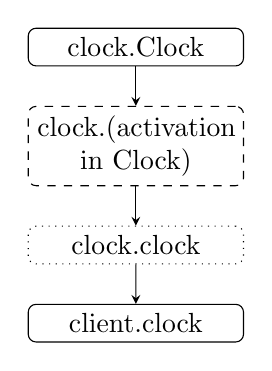
\begin{tikzpicture}[
    arrowstyle/.style={draw, -stealth},
    edge from parent/.style={draw, -stealth},
    reaction/.style={rectangle, draw, rounded corners=1mm, text width=2.5cm,
        text centered, anchor=north},
    activation/.style={rectangle, draw, rounded corners=1mm, dashed, text width=2.5cm,
        text centered, anchor=north},
    push/.style={rectangle, draw, rounded corners=1mm, dotted, text width=2.5cm,
        text centered, anchor=north},
    level 1/.style={sibling distance=7.0cm},
    level 2/.style={sibling distance=4.0cm},
    level 3/.style={sibling distance=3.0cm},
    level distance=0.5cm, growth parent anchor=south
]
\node (Action) [reaction] {clock.Clock}
  child {
    node (Activation01) [activation] {clock.(activation in Clock)}
    child {
      node (Push01) [push] {clock.clock}
      child {
        node (Reaction01) [reaction] {client.clock}
      }
    }
  }
;
\end{tikzpicture}
\endgroup
%%}%
\cprotect\caption{Transaction diagram for the \verb+clock.Clock+ action of the Clock System}
\label{clock_transaction}
\end{figure}

\section{Properties of Composition}
\label{propcomp}
In this section, we examine various features related to reactive components and composition.
Substitutional equivalence for reactive components is demonstrated by outlining a procedure for in-lining sub-components.
Hazards of composition, namely, non-deterministic state transitions resulting from conflicting and recursive composition, are identified and a means of detecting them is proposed.
The issue of decomposition is considered and \emph{pull ports} are introduced as a mechanism for decomposition.

\begin{figure}
\begin{verbatim}
component System {
  /* Substitution of clock component. */
  var int clock_counter (0)
  var bool clock_flag (false)
  push clock_clock(int t)

  reaction clock_request() clock_flag := true

  clock_Clock: clock_flag -> clock_flag := false activates clock_clock(clock_counter)

  clock_Tick: clock_counter := clock_counter + 1

  /* Substitution of client component. */
  var bool client_flag (false)
  push client_request()

  client_Request: !client_flag -> client_flag := true activates client_request()

  reaction client_clock(int t) client_flag := false || /* do something with t */

  bind {
    client_request -> clock_request
    clock_clock -> client_clock
  }
}
\end{verbatim}
\caption[Substitution of sub-components for the Clock System]{Substitution of state variables, ports, actions, and reactions for the sub-components of the System component of the Clock System}
\label{se1}
\end{figure}

\begin{figure}
\begin{verbatim}
component System {
  var int clock_counter (0)
  var bool clock_flag (false)
  var bool client_flag (false)
  push clock_clock(int t)
  push client_request()

  clock_Clock: clock_flag -> clock_flag, client_flag :=
    false, false activates clock_clock(clock_counter) ||
    /* do something with clock_counter */

  client_Request: !client_flag -> client_flag, clock_flag :=
    true, true activates client_request()

  clock_Tick: clock_counter := clock_counter + 1
}
\end{verbatim}
\caption[Simplification of expanded System component of the Clock System]{Simplifications of ports, bindings, and transitions in the expanded System component of the Clock System}
\label{se2}
\end{figure}

\subsection{Substitutional Equivalence}
\label{substitutional_equivalence}
For reactive components, substitutional equivalence means that a sub-component can be replaced with its definition and the result is a well-defined entity in the model.
To this end, a procedure for substituting the definition of a sub-component involves 1) renaming and adding all state variables, ports, actions, and reactions to the parent component and 2) simplifying bindings by substituting the transitions associated with a reaction into the action or reaction that activates the reaction in question.

To illustrate, Figure~\ref{se1} shows the result of substituting state variables, ports, actions, and reactions into the System component of Figure~\ref{system_component}.
Identifiers in the sub-components have been prefixed with the name of the sub-component instance to avoid name clashes.
For example, the \verb+request+ reaction in the \verb+clock+ sub-component has been renamed to \verb+clock_request+.
Figure~\ref{se2} shows the result of simplifying bindings and state transitions.
Note that the push ports have been retained for subsequent composition, i.e., the System component may be a component in a larger system.
The result is a reactive component whose ``size'' in terms of state variables, actions, and reactions is the sum of the sizes  of its constituent components.
Substituting the definition of the Clock component and Client components into the System component confirms the intuition that the flag variable in the client and flag variable in the clock are the same since 1) initially they have the same value and 2) they take on the same value in every state transition.

\subsection{Determinism and Composition}
\label{determinism}

\begin{figure}
\centering
%%\resizebox{\textwidth}{!}{%
\begingroup
\fontsize{10pt}{12pt}\selectfont
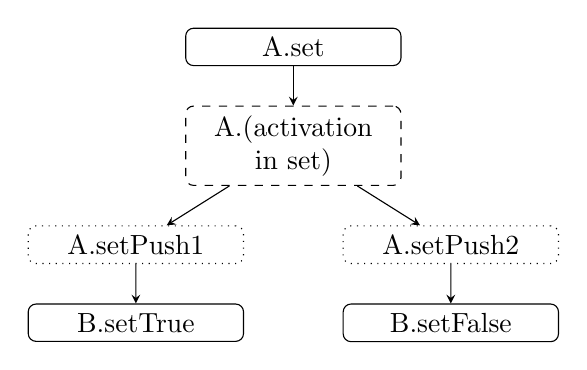
\begin{tikzpicture}[
    arrowstyle/.style={draw, -stealth},
    edge from parent/.style={draw, -stealth},
    reaction/.style={rectangle, draw, rounded corners=1mm, text width=2.5cm,
        text centered, anchor=north},
    activation/.style={rectangle, draw, rounded corners=1mm, dashed, text width=2.5cm,
        text centered, anchor=north},
    push/.style={rectangle, draw, rounded corners=1mm, dotted, text width=2.5cm,
        text centered, anchor=north},
    level 1/.style={sibling distance=7.0cm},
    level 2/.style={sibling distance=4.0cm},
    level 3/.style={sibling distance=3.0cm},
    level distance=0.5cm, growth parent anchor=south
]
\node (Action) [reaction] {A.set}
  child {
    node (Activation01) [activation] {A.(activation in set)}
    child {
      node (Push01) [push] {A.setPush1}
      child {
        node (Reaction01) [reaction] {B.setTrue}
      }
    }
    child {
      node (Push02) [push] {A.setPush2}
      child {
        node (Reaction02) [reaction] {B.setFalse}
      }
    }
  }
;
\end{tikzpicture}
\endgroup
%%}%
\caption{Transaction diagram for a non-deterministic transaction}
\label{ndt}
\end{figure}

The result of composing two well-defined reactive components may yield a system that is non-deterministic.
The two ``hazards'' that must be avoided are non-deterministic assignment to state variables and recursively activated reactions.
Non-deterministic assignment results when the next value for a state variable is not well defined due to the inclusion of two or more transitions in a transaction that operate on the state variable.
To illustrate, consider the transaction depicted in Figure~\ref{ndt}.
The set action of component A has a single activation that activates both the setPush1 and setPush2 push ports.
The setPush1 port is bound to the setTrue reaction of component B while the setPush2 port is bound to the setFalse reaction of the same component B.
Suppose that the setTrue reaction sets a flag to true while the setFalse reaction sets the same flag to false.
The transaction is non-deterministic because the value of the flag after the (A,set) transaction may either be true or false.
An offending pair of transitions may appear anywhere in a transaction graph given that arbitrary transaction graphs may be constructed through composition.
If the underlying language used to define transitions admits pointers, dynamic memory, if statements, and loops (i.e., is Turing-complete), then the problem of determining if two transitions operate on the same state variable is undecidable in general~\cite{Landi:1992:USA:161494.161501, Ramalingam:1994:UA:186025.186041}.
For a transaction graph $G$, instances $i_1$ and $i_2$, and actions/reactions $t_1$ and $t_2$, a necessary (but not sufficient) condition for non-deterministic assignment $\mathit{NDA}$ from composition is $\mathit{NDA}(G): \exists (i_1, t_1), (i_2, t_2) \in G.N, i_1 = i_2, t_1 \ne t_2$ which says that the transaction must contain two different transitions involving the same component instance.

A recursively activated transition occurs when the transaction graph has a cycle.
The execution of such a transaction may result in well-defined next values for all state variables assuming that 1)~the recursion is bounded and 2)~the parameters passed to every reaction result in identical computations.
A transaction may be analyzed like a traditional transformational program since it has finite input, a finite output, and should terminate.
The first problem, then, is a thinly disguised version of the halting problem since it asks if a computation (the transaction) expressed in a Turing-complete language terminates (has bounded recursion)~\cite{Turing01011937, davis1958computability}.
A bounded recursion means that the execution of the transaction will generate a bounded number of activations $A$.
For each activation $a \in A$, we must determine what state is updated by $a$.
If the language is Turing-complete, then this problem is undecidable in general~\cite{Landi:1992:USA:161494.161501, Ramalingam:1994:UA:186025.186041}.
For state variables that are updated by more than one activation, we must then show that each activation sets the state variable to the exact same next state.
If we treat each activation as a program, then we require a function that determines if two (arbitrary) programs compute the same function, which is again, undecidable in general~\cite{Rice:53}.

The difficulty of detecting composition that results in non-deterministic assignments suggests that these problems are best checked by a machine.
That is, an implementation of reactive components may prevent non-deterministic assignment by checking that $\mathit{NDA}(G)$ is false for all transaction graphs in the system.
Similarly, an implementation may check for recursive activation by checking for cycles in transaction graphs.
Both of these approaches are used by the implementation described in Section~\ref{sound_composition}.

\subsection{Decomposition, Getters, and Pull Ports}
\label{decomposition}
Substitutional equivalence implies that the process of substituting the definition of a sub-component into a parent component may be reversed and that sub-components may be ``factored out'' of an existing component, e.g., for reuse with other components.
%% One motivation for extracting sub-components is to support the software engineering practice of refactoring where common code is extracted so that it can be reused in various places.

Another motivation for decomposition is potentially increased performance through parallelism.
Recall that true concurrency in reactive components is modeled as the serial and non-deterministic execution of atomic actions.
Two transactions can be safely executed concurrently if it can be shown that the state variables involved in each transaction are disjoint.
As was previously mentioned, making this determination is undecidable for Turing-complete languages in the general case.
However, the problem becomes decidable if the component instance is used as a proxy for its constituent state variables.
Let $\mathit{rw}: t \to \{ \mathit{Read}, \mathit{Write} \}$ be a function that maps a transition to a value indicating that variables are read-only during the transition or written in some way.
Two instance/transition pairs are independent ($\mathit{indp}$) if either the instances are different or at most one of the transitions writes to the variables of the instance:
\begin{equation}
\mathit{indp}((i_1, t_1), (i_2, t_2)): i_1 \ne i_2 \lor \lnot (\mathit{rw}(t_1) = \mathit{Write} \land \mathit{rw}(t_2) = \mathit{Write})
\end{equation}
Two transaction graphs are independent if all of their nodes are independent $\mathit{indp}(G_1, G_2) = \forall (i_1, t_1) \in G_1.N, (i_2, t_2) \in G_2.N \; \mathit{indp}((i_1, t_1), (i_2, t_2))$.
The significance of the preceding analysis is that the determination about what actions can be executed concurrently becomes machine checkable due to the strong guarantee that state variables belonging to an instance can only be modified by the transitions of that instance.

To illustrate the mechanisms required for decomposition, we will factor out a Counter component from the Clock component of Figure~\ref{clock_component} and then rewrite the Clock component using the Counter component.
Upon inspection, the \verb+Tick+ action and \verb+request+ reaction can be executed concurrently since the state variables involved in each transition are disjoint.
Figure~\ref{counter_component} shows the Counter component which consists of a \verb+counter+ state variable.
The \verb+Tick+ action can be moved to the Counter component without complication.
The \verb+Clock+ action of the Clock component \emph{reads} the value of \verb+counter+ which suggests that a mechanism for accessing the state variables in a component is required.
Thus, we introduce the notion of a \emph{getter} method which can be called on a component to produce a value that may be derived from its state variables.
In the Counter component, the \verb+getCounter+ getter returns the current value of the counter.
A getter is not allowed to modify the state of a component and may only be invoked in the immutable phase.
These semantics preserve the strict separation of immutable phase and mutable phase.
When analyzing composition, a getter is treated like a transition that reads the state variable of the corresponding instance.
Figure~\ref{factored_clock_component} shows the Clock component rewritten to use a Counter sub-component and a getter.

\begin{figure}
\begin{verbatim}
component Counter {
  var int counter (0)

  Tick: counter := counter + 1

  getCounter() int {
    return counter
  }
}
\end{verbatim}
\caption{Definition of the Counter component of the Factored Clock System}
\label{counter_component}
\end{figure}

\begin{figure}
\begin{verbatim}
component Clock {
  var Counter c
  var bool flag (false)
  push clock(int t)

  reaction request() flag := true

  Clock: flag -> flag := false activates clock(c.getCounter())
}
\end{verbatim}
\caption{Definition of the Clock component of the Factored Clock System}
\label{factored_clock_component}
\end{figure}

The logic associated with the \verb+flag+ state variable represents a generic request-response protocol except for the call to \verb+c.getCounter()+.
To indirect the call to \verb+c.getCounter()+ we introduce the notion of a \emph{pull port}.
A pull port represents an external value dependency.
A component can demand a value from the pull port in the immutable phase.
Like push ports, pull ports have an active and passive side.
The active side represents the caller and the passive side represents the callee.
Getters are sufficient to realize the passive side of a pull port.
Every active pull port must be bound to exactly one passive pull port via composition.
Figure~\ref{request_response_component} shows a component that implements the request-response protocol using a pull port \verb+getValue+.
Figure~\ref{factored2_clock_component} shows the Clock component written in terms of the Counter and RequestResponse components.
An \verb+export+ directive allows reactions, getters, and ports in sub-components to be available in the interface of the encapsulating component.

\begin{figure}
\begin{verbatim}
component RequestResponse {
  var bool flag (false)
  pull getValue() int
  push response(int t)

  reaction request() flag := true

  Response: flag -> flag := false activates response(getValue())
}
\end{verbatim}
\caption{Definition of the RequestResponse component of the Factored Clock System}
\label{request_response_component}
\end{figure}

\begin{figure}
\begin{verbatim}
component Clock {
  var Counter c
  var RequestResponse rr
  push request()
  push clock(int t)

  bind {
    c.getCounter -> rr.getValue
  }

  export rr.request as request
  export rr.response as clock
}
\end{verbatim}
\caption{Definition of the Clock component of the Factored Clock System (fully-factored)}
\label{factored2_clock_component}
\end{figure}

Pull ports are subject to a hazard of composition similar to the recursive activation hazard of push ports.
A cycle in the graph of composed pull ports is equivalent to a recursively defined function.
The recursion may be bounded but this is undecidable in the general case.
Consequently, an implementation may reject recursively defined getters and pull ports.

\section{Summary}
In this chapter, we have presented the reactive component model for reactive programs.
A reactive component consists of a set of state variables and transitions that are private to the component.
The interface of a reactive component consists of push ports and reactions, which allow a component to trigger a transition in another component, and pull ports and getters, which allow a component to access the state of another component.
The external or visible behavior of a reactive component can be traced through its interface, specifically its push ports.
The internal details of a component can often be abstracted away to permit reasoning about the behavior of a composed system at various levels of detail.
Composition is achieved through recursive encapsulation (sub-components) and explicit port binding and satisfies the requirements for principled composition set forth in Section~\ref{challenges}.
As demonstrated in Section~\ref{substitutional_equivalence}, the definitions of sub-components can be substituted into the containing component resulting in an equivalent system (substitutional equivalence).
Similarly, sub-components may be ``factored out'' by using pull ports and getters to safely access the state of the sub-components.

The private nature of state variables and transitions causes properties established from the text of a component to be preserved through composition.
Composition links transitions to form an atomic transaction that allows the properties of one component to be related to another component.
When the sub-components of a component are protected from further composition, the properties derived from their interactions are preserved as the parent component is composed.
Property-preserving composition is essential for reasoning about systems in a hierarchical and/or modular fashion.

The result of composing reactive components is either well-defined due to the atomic nature of transactions or illegal due to the composition hazards of recursive transactions and non-deterministic state transitions.
Analysis of these hazards at the state variable level is impossible due to the undecidable nature of their sub-problems.
This suggests that implementations may restrict composition to prevent the conditions necessary for recursive transactions and non-deterministic state transitions.
The main concession is allowing a component instance to proxy for its state variables.
The problem of detecting recursive transactions, then, can be posed as the problem of detecting cycles in a directed graph.
Similarly, the problem of detecting potentially non-deterministic state transitions is reduced to a set membership problem.
Valid systems that fail the check for non-deterministic state transitions using component instance proxies can be refactored by decomposing  the offending components.

  }%

\end{frame}

\begin{frame}[fragile]{\rcgo{}:  Keywords for Defining Components}

{\small
\begin{lstlisting}
type Clock component {
  counter uint;
  flag bool;
  response push (t uint);     // active
  counter pull () uint;       // active
};

init (c *Clock) Initialize () {.}
action (c $const *Clock) Respond (this.flag) {.}
reaction (c $const *Clock) Request () {.}
getter (c $const *Counter) Counter () uint {.}

bind (s *System) BindAll {
  s.sampler.Request -> s.clock.Request;
  s.clock.counter   <- s.counter.Counter;
}

instance s System Initialize ();
\end{lstlisting}
}

\onslide<2>
\begin{tikzpicture}[overlay,remember picture]
  \pgftransformshift{\pgfpointanchor{current page}{center}}
  \node [draw, rectangle, minimum height=15, minimum width=60, red] at (-1.9,3.5) {};
\end{tikzpicture}

\onslide<3->
\begin{tikzpicture}[overlay,remember picture]
  \pgftransformshift{\pgfpointanchor{current page}{center}}
  \node [draw, cylinder, shape border rotate=90, minimum height=20, minimum width=20, fill=white] (sv1) at (-1.5,2.75) {};
\end{tikzpicture}

\onslide<4>
\begin{tikzpicture}[overlay,remember picture]
  \pgftransformshift{\pgfpointanchor{current page}{center}}
  \node [draw, rectangle, minimum height=15, minimum width=35, red] at (-2.5,2.25) {};
\end{tikzpicture}

\onslide<4->
\begin{tikzpicture}[overlay,remember picture]
  \pgftransformshift{\pgfpointanchor{current page}{center}}
  \node [shape=rightout, draw, text=white, fill=white] at (1, 2.3) {man};
\end{tikzpicture}

\onslide<5>
\begin{tikzpicture}[overlay,remember picture]
  \pgftransformshift{\pgfpointanchor{current page}{center}}
  \node [draw, rectangle, minimum height=15, minimum width=35, red] at (-2.7,1.8) {};
\end{tikzpicture}

\onslide<5->
\begin{tikzpicture}[overlay,remember picture]
  \pgftransformshift{\pgfpointanchor{current page}{center}}
  \node [shape=leftin, draw, text=gray, fill=gray] at (.4,1.8) {man};
\end{tikzpicture}

\onslide<6>
\begin{tikzpicture}[overlay,remember picture]
  \pgftransformshift{\pgfpointanchor{current page}{center}}
  \node [draw, rectangle, minimum height=15, minimum width=35, red] at (-5,.6) {};
\end{tikzpicture}

\onslide<7->
\begin{tikzpicture}[overlay,remember picture]
  \pgftransformshift{\pgfpointanchor{current page}{center}}
  \node [draw, diamond, minimum height=15, minimum width=20, fill=white] at (3.1,.5) {};
  \node [draw, minimum height=15, minimum width=20, rounded corners=5, fill=white] at (4.88,.6) {};
\end{tikzpicture}

\onslide<7>
\begin{tikzpicture}[overlay,remember picture]
  \pgftransformshift{\pgfpointanchor{current page}{center}}
  \node [draw, rectangle, minimum height=15, minimum width=45, red] at (-4.8,.1) {};
\end{tikzpicture}

\onslide<8->
\begin{tikzpicture}[overlay,remember picture]
  \pgftransformshift{\pgfpointanchor{current page}{center}}
  \node [shape=leftin, draw, text=white, fill=white] at (4,-.25) {man};
\end{tikzpicture}

\onslide<8>
\begin{tikzpicture}[overlay,remember picture]
  \pgftransformshift{\pgfpointanchor{current page}{center}}
  \node [draw, rectangle, minimum height=15, minimum width=55, red] at (-4.5,-.3) {};
\end{tikzpicture}

\onslide<9->
\begin{tikzpicture}[overlay,remember picture]
  \pgftransformshift{\pgfpointanchor{current page}{center}}
  \node [shape=rightout, draw, text=gray, fill=gray] at (6, -.7) {man};
\end{tikzpicture}

\onslide<9>
\begin{tikzpicture}[overlay,remember picture]
  \pgftransformshift{\pgfpointanchor{current page}{center}}
  \node [draw, rectangle, minimum height=15, minimum width=50, red] at (-4.75,-.7) {};
\end{tikzpicture}

\onslide<10->
\begin{tikzpicture}[overlay,remember picture]
  \pgftransformshift{\pgfpointanchor{current page}{center}}
  \draw[thick] (4,-2.1) -- (6,-2.1);
\end{tikzpicture}

\onslide<10>
\begin{tikzpicture}[overlay,remember picture]
  \pgftransformshift{\pgfpointanchor{current page}{center}}
  \node [draw, rectangle, minimum height=15, minimum width=40, red] at (-5,-1.5) {};
\end{tikzpicture}

\onslide<11->
\begin{tikzpicture}[overlay,remember picture]
  \pgftransformshift{\pgfpointanchor{current page}{center}}
  \node [rectangle, draw, minimum height=15, minimum width=20, fill=white] at (2.1, -3.625) {};
\end{tikzpicture}

\onslide<11>
\begin{tikzpicture}[overlay,remember picture]
  \pgftransformshift{\pgfpointanchor{current page}{center}}
  \node [draw, rectangle, minimum height=15, minimum width=55, red] at (-4.5,-3.65) {};
\end{tikzpicture}

\end{frame}

\begin{frame}{Model $\to$ Language}
  \centering

  \resizebox{\textwidth}{!}{%
    \chapter{Reactive Component Model}
\label{model}

In this chapter, we present a new model for composing and decomposing reactive programs via \emph{reactive components}.
The model is biased toward practical software development even as it enforces properties based in formal methods.
Consequently, the model favors utility, practicality, flexibility, and ease of implementation.
Unlike UNITY in which composition is not property-preserving, the composition of reactive components is property-preserving which facilitates hierarchical and modular reasoning.
Unlike I/O Automata in which transitions have limited depth, a transition among reactive components may access and cascade to an arbitrary number of other components, which permits decomposition to an arbitrary depth and degree.

%% \paragraph{Formal models and software engineering.}
%% I claim that most of the software that is ``put into production'' will never be proved formally correct.
%% This is a function of economics since modeling and constructing proofs is a labor-intensive process that can only be justified for safety or mission critical software.
%% However, I would argue that the development and application of formal models are critical to software engineering.
%% To illustrate, consider \emph{structured programming}~\cite{dahl1972structured}.
%% Structured programming assumes an abstract machine that executes programs that are restricted to a small set of well-defined control structures and assignment statements.
%% A program written in this form can be reasoned about directly from the text by formulating a Hoare-triple for each statement.
%% Structured programming opened the door for \emph{structured programming languages} which are also based on well-defined control structures and evaluation semantics.
%% Thus, while very few programmers will prove their structured programs correct, all of them informally use structured programming when they are fixing a bug revealed by a unit test or analyzing a core dump in a debugger.
%% Structured programming languages reduced the accidental complexity associated with writing the same program in assembly language.

%% The realm of reactive programs is waiting for a similar reduction in accidental complexity.
%% Taking a hint from structured programming, I believe two things are required.
%% First, we must write reactive programs against an easy-to-reason-about abstract machine instead of low-level interfaces like atomic instructions and thread libraries.
%% Second, we must restrict the form of reactive programs so that they can be reasoned about from the text.
%% I hope the proposed model of reactive systems is a step toward toward this goal.

\section{Features of the Model}

%% left active pull port
%% x, y, width, height, label
\def\lapull[#1,#2,#3,#4,#5,#6]#7{
  \draw [fill=lightgray] (#1,#2) -- ++(${#4*.5}*(-1,0) + {#4*.5}*(0,-1)$) -- ++($#3*(1,0)$) -- ++($#4*(0,1)$) -- ++($#3*(-1,0)$) -- cycle;
  \node (#5) at (#1,#2) {};
  \node (#6) at ($(#1,#2) + {#3 - .5 * #4}*(1,0)$) {};
  \node [right, align=left] at (#1,#2) {#7};
}

%% left active push port
%% x, y, width, height, label
\def\lapush[#1,#2,#3,#4,#5,#6]#7{
  \draw [fill=white] ($(#1,#2) + {#4*.5}*(-1,0)$) -- ++(${#4*.5}*(1,0) + {#4*.5}*(0,-1)$) -- ++($#3*(1,0)$) -- ++($#4*(0,1)$) -- ++($#3*(-1,0)$) -- cycle;
  \node (#5) at ($(#1,#2) - .5*#4*(1,0)$) {};
  \node (#6) at ($(#1,#2) + {#3}*(1,0)$) {};
  \node [right, align=left] at (#1,#2) {#7};
}

%% left passive pull port
%% x, y, width, height, label
\def\lppull[#1,#2,#3,#4,#5,#6]#7{
  \draw [fill=lightgray] ($(#1,#2) + {#4*.5}*(-1,0)$) -- ++(${#4*.5}*(1,0) + {#4*.5}*(0,-1)$) -- ++($#3*(1,0)$) -- ++($#4*(0,1)$) -- ++($#3*(-1,0)$) -- cycle;
  \node (#5) at ($(#1,#2) - .5*#4*(1,0)$) {};
  \node (#6) at ($(#1,#2) + {#3}*(1,0)$) {};
  \node [right, align=left] at (#1,#2) {#7};
}

%% left passive push port
%% x, y, width, height, label
\def\lppush[#1,#2,#3,#4,#5,#6]#7{
  \draw [fill=white] (#1,#2) -- ++(${#4*.5}*(-1,0) + {#4*.5}*(0,-1)$) -- ++($#3*(1,0)$) -- ++($#4*(0,1)$) -- ++($#3*(-1,0)$) -- cycle;
  \node (#5) at (#1,#2) {};
  \node (#6) at ($(#1,#2) + {#3 - .5*#4}*(1,0)$) {};
  \node [right, align=left] at (#1,#2) {#7};
}

%% right passive pull port
%% x, y, width, height, label
\def\rppull[#1,#2,#3,#4,#5,#6]#7{
  \draw [fill=lightgray] ($(#1,#2) + {#4*.5}*(1,0)$) -- ++(${#4*.5}*(-1,0) + {#4*.5}*(0,-1)$) -- ++($#3*(-1,0)$) -- ++($#4*(0,1)$) -- ++($#3*(1,0)$) -- cycle;
  \node (#5) at ($(#1,#2) + {#4*.5}*(1,0)$) {};
  \node (#6) at ($(#1,#2) + {#3}*(-1,0)$) {};
  \node [left] at (#1,#2) {#7};
}

%% right active push port
%% x, y, width, height, label
\def\rapush[#1,#2,#3,#4,#5,#6]#7{
  \draw [fill=white] ($(#1,#2) + {#4*.5}*(1,0)$) -- ++(${#4*.5}*(-1,0) + {#4*.5}*(0,-1)$) -- ++($#3*(-1,0)$) -- ++($#4*(0,1)$) -- ++($#3*(1,0)$) -- cycle;
  \node (#5) at ($(#1,#2) + {#4*.5}*(1,0)$) {};
  \node (#6) at ($(#1,#2) + {#3}*(-1,0)$) {};
  \node [left] at (#1,#2) {#7};
}

%% right passive push port
%% x, y, width, height, label
\def\rppush[#1,#2,#3,#4,#5,#6]#7{
  \draw [fill=white] (#1,#2) -- ++(${#4*.5}*(1,0) + {#4*.5}*(0,-1)$) -- ++($#3*(-1,0)$) -- ++($#4*(0,1)$) -- ++($#3*(1,0)$) -- cycle;
  \node (#5) at (#1,#2) {};
  \node (#6) at ($(#1,#2) + {#3 - .5*#4}*(-1,0)$) {};
  \node [left] at (#1,#2) {#7};
}

%% right active pull port
%% x, y, width, height, label
\def\rapull[#1,#2,#3,#4,#5,#6]#7{
  \draw [fill=lightgray] (#1,#2) -- ++(${#4*.5}*(1,0) + {#4*.5}*(0,-1)$) -- ++($#3*(-1,0)$) -- ++($#4*(0,1)$) -- ++($#3*(1,0)$) -- cycle;
  \node (#5) at (#1,#2) {};
  \node (#6) at ($(#1,#2) + {#3 - .5*#4}*(-1,0)$) {};
  \node [left] at (#1,#2) {#7};
}

\begin{figure}[H]
\centering
\resizebox{\textwidth}{!}{%
\begingroup
\fontsize{10pt}{12pt}\selectfont
\begin{tikzpicture}
[
arrowstyle/.style={
  decoration={markings,mark=at position 1 with {\arrow[scale=2,]{stealth}}},
  postaction={decorate},
  shorten >=0.4pt
}
]

%% component boundary
\draw (0,0) rectangle (10,8.25);
%% active pull ports
\lapull[0,1.5,1,.5,apullex1,apullin1]{}
\node[align=center] at (-1,1.5) {active\\pull port};
\lapull[0,.5,1,.5,apullex2,apullin2]{}
%% passive pull ports
\rppull[10,1.5,1,.5,ppullex1,ppullin1]{}
\node[align=center] at (11,1.5) {passive\\pull port};
\rppull[10,.5,1,.5,ppullex2,ppullin2]{}
\draw[thick] (apullin2.center) -- (ppullin2.center);
%% actions and rections
\node[draw, diamond, minimum height=15, minimum width=20] (pre) at (2.5,3) {};
\node at (2.5,2.5) {precondition};
\node[draw, minimum height=15, minimum width=50, rounded corners=5] (trans1) at (5,3) {};
\draw[dashed] (3.5,3) ellipse (3 and 1);
\node at (3.5,3.5) {\textbf{\emph{action}}};
\node[draw, minimum height=15, minimum width=50, rounded corners=5] (trans2) at (5,5) {};
\node at (5,4.5) {transition};
\draw[thick,arrowstyle] (pre) -- (trans1);
\draw[thick] (apullin1.center) -| (trans1) node[pos=.5,right] {\textbf{call}};
%% active push ports
\rapush[10,3,1,.5,apushex1,apushin1]{}
\rapush[10,4,1,.5,apushex2,apushin2]{}
\rapush[10,5,1,.5,apushex3,apushin3]{}
\node[align=center] at (11.1,5) {active\\push port};
\draw[thick,dashed,arrowstyle] (trans1) -- (apushin1.center);
\draw[thick,dashed,arrowstyle] (trans1) -- (apushin2.center);
\node at(7.5,4) {\textbf{activate}};
\draw[thick,dashed,arrowstyle] (trans2) -- (apushin2.center);
\draw[thick,dashed,arrowstyle] (trans2) -- (apushin3.center);
%% passive push ports
\lppush[0,5,1,.5,ppushex1,ppushin1]{}
\draw[thick,arrowstyle] (ppushin1.center) -- (trans2);
\node[align=center] at (-1.1,5) {passive\\push port};
\draw[dashed] (2,5) ellipse (5 and 1);
\node at (2,5.5) {\textbf{\emph{reaction}}};
\node[draw, cylinder, shape border rotate=90, minimum height=40, minimum width=40] (sv1) at (5,7.25) {};
\node[align=center] at (5,6.25) {state variables};
\end{tikzpicture}
\endgroup
}%
\caption{Features of a reactive component\label{reactive_component}}
\end{figure}

Figure~\ref{reactive_component} shows the major features of a reactive component.
As in other state-based formal models like UNITY~\cite{chandy1989parallel} and I/O Automata~\cite{nancy1996distributed}, the core of a reactive component in this model is a set of \emph{state variables} and a set of atomic \emph{transitions} that manipulate those state variables.
When reasoning about a system, behavior is expressed as propositions over the state variables where the propositions are derived from the transitions.

%% The contribution that this work makes to existing state-based formal models of reactive systems is a combination of interface elements and composition semantics that allow reactive programs to be composed in a principled way.

The reactive component model defines interface elements and composition semantics that allow reactive programs to be composed in a principled way.
For example, an \emph{active push port} allows a transition in one component to be linked to a transition in another component such that the resulting combined transition is atomic.
Active push ports allow reactive components to publicize their behavior.
An active push port may be \emph{bound} to and conditionally \emph{activate} zero or more \emph{passive push ports}.
A passive push port names the corresponding transition that will be executed when the passive push port is activated.
This combination of passive push port and transition is called a \emph{reaction} because it reacts to a transition in another component.

The atomic linkage of a transition in one component to a transition in another component through the push port mechanism allows the properties of each component to be related to one another and more complex systems to be constructed by composing simpler systems.
Transitions that are not executed via a passive push port are executed by the scheduler.
A transition of this kind may be governed by a Boolean expression called a \emph{precondition}.
The combination of a precondition and transition is called an \emph{action} because it is a voluntary transition under the control of the containing component.

An \emph{active pull port} represents an immutable external data dependency.
The component may \emph{call} an active pull port to yield a value required in a transition.
Active pull ports must be bound to a \emph{passive pull port} which resembles a function returning a value, e.g., a getter or a predicate.
Where push ports allow components to publicize their behavior, pull ports allow components to safely publicize their internal state for use by other components.

Composition in the reactive component model has two main features.
The first is recursive encapsulation where a state variable in one component may represent an instance of another reactive component.
The second is the ability to bind push ports and pull ports through an \emph{explicit} set of \emph{bindings}.
The decision to use an explicit set of bindings (as opposed to implicit named-based matching) is more in keeping with the goals and techniques of practical software development, since it facilitates the use of software developed under different naming conventions, i.e., third-party software.
A third minor feature called \emph{exporting} is the ability of an encapsulating component to adopt interface elements of its sub-components without defining complimentary ports and transitions that do nothing but forward an activation or call.
The ability to publicize behavior and state and the ability to assemble well-defined behavior from existing behaviors in a straight-forward and flexible way are thus defining characteristics of the reactive component model.

\begin{figure}
\centering
\resizebox{\textwidth}{!}{%
\begingroup
\fontsize{10pt}{12pt}\selectfont
\begin{tikzpicture}
\draw (0,6.5) rectangle (5,10);
\node[below] at (2.5,10) {Web Server};
\rapull[5,9,3.4,.5,ex1a,ignore]{verify(HttpHeader)};
\rapush[5,8,3.6,.5,ex2a,ignore]{request(HttpRequest)};
\rppush[5,7,4.2,.5,ex3a,ignore]{respond(HttpResponse)};

\draw(6,2.5) rectangle (11,10);
\node[below] at (8.5,10) {Application Logic};
\lppull[6,9,3.4,.5,ex1b,ignore]{verify(HttpHeader)};
\lppush[6,8,3.8,.5,ex2b,ignore]{request(HttpRequest)};
\lapush[6,7,3.9,.5,ex3b,ignore]{respond(HttpResponse)};

\rapush[11,6,3.5,.5,ex4a,ignore]{request(DBRequest)};
\rppush[11,5,4.1,.5,ex5a,ignore]{respond(DBResponse)};

\rapush[11,3,2.4,.5,ex6a,ignore]{log(Message)};

\draw (12,4.5) rectangle (17,7);
\node[below] at (14.5,7) {Database};
\lppush[12,6,3.7,.5,ex4b,ignore]{request(DBRequest)};
\lapush[12,5,3.8,.5,ex5b,ignore]{respond(DBResponse)};

\draw (12,2.5) rectangle (17,4);
\node[below] at (14.5,4) {Logging Service};
\lppush[12,3,2.5,.5,ex6b,ignore]{log(Message)};

\draw (ex1a.center) -- (ex1b.center);
\draw (ex2a.center) -- (ex2b.center);
\draw (ex3a.center) -- (ex3b.center);
\draw (ex4a.center) -- (ex4b.center);
\draw (ex5a.center) -- (ex5b.center);
\draw (ex6a.center) -- (ex6b.center);

\end{tikzpicture}
\endgroup
}%
\caption{Diagram of a web application built using reactive components\label{web_server}}
\end{figure}

To demonstrate the utility of component interfaces and explicit support for property-preserving composition, we now present an illustrative design for a web application using reactive components, as is shown in Figure~\ref{web_server}.
The web application consists of five reactive components.
The first is an unnamed top-level component representing the complete application.
This component has four sub-components representing a web server, the application logic, a database, and a logging service.
The ports of the application logic component have been bound to the corresponding ports in the web server, database, and logging service components.
The interface of a component, which consists of its ports, provides insight into the behavior of the component.
For example, based on the interface of the web server component we may expect it to 1)~verify incoming HTTP requests\footnote{A production web server may verify that the requested HTTP method can be applied to the given URI, that content length limits are respected, that content types are supported, etc.}, 2)~pass on valid HTTP requests to the application, and 3)~accept HTTP responses from the application.

Figure~\ref{web_server} also demonstrates how reactive programs can be constructed by composing reactive components, so that a developer may focus on the application logic and use existing components for the web server, database, and logging service.
Furthermore, one can imagine developing three stateless components surrounding the application logic that do nothing but translate messages between application specific message types and the generic types required by the web server, database, and logging service.
The application logic, then, is completely isolated from the surrounding libraries and may be tested by providing mock components for the web server, database, and logging service.
The application logic itself has a well-defined interface and could be reused, say, by implementing a graphical front-end to drive the application instead of a web service.

\subsection{State Variables}
Part of the internal core of a reactive component is a set of state variables, which are the subject of the propositions that demonstrate the behavior of the system.
The state variables are manipulated by the assignment statements that constitute the transitions.
As in other formal models, the types of the state variables may be selected to make writing proofs easier.
%% That is, the state variables have mathematically friendly types like integers, sets, and lists.
However, implementations of the reactive component model must provide a concrete type system that allows the state variables to be realized on a given machine.
For example, the \rcgo{} language for reactive components presented in Chapter~\ref{language} of this dissertation uses the type system of Go to define the types of state variables.
The type of a state variable also may be a reactive component type, which facilitates recursive encapsulation.
For modeling purposes, state variables typically have \emph{value semantics} to avoid reasoning about references and aliasing.
However, and as a practical concession, we will introduce pointers for building arbitrary linked data structures (since we advocate an imperative state-based implementation) and discuss issues raised by introducing pointers into the reactive component model in Chapter~\ref{language}.

\subsection{Atomic State Transitions}
The rest of the internal core of a reactive component is a set of atomic state transitions that manipulate the state variables.
A precise definition of the atomicity of state transitions will be deferred to the subsequent sections on composition (Section~\ref{composition}) and execution (Section~\ref{execution}).
State variables and state transitions are private, meaning that transitions can only refer to the state variables of the associated reactive component and a transition in one reactive component can only be linked to a transition in another component through the composition mechanisms.
Thus, all initialization and updates to state variables can be determined by examining the transitions of the corresponding component.
The encapsulation of state variables contribute to composition being \emph{compositional}.
All properties established from the transitions of a component will continue to hold as the component participates in composition since the set of transitions that affect the state variables is fixed.
State transitions must be deterministic meaning that the next value of every state variable is uniquely and well defined.
State transitions defined by a sequence of simple assignments are implicitly deterministic.
However, special care must be take to ensure that state transitions are deterministic when described using parallel assignment statements as the same variable may appear on the left-hand-side and be assigned two different values~\cite{chandy1989parallel}.
As described in Sections~\ref{composition} and \ref{execution}, composition links transitions using parallel assignment which creates an opportunity for non-deterministic state transitions.
The problem of non-deterministic state transitions arising from composition is explored in Section~\ref{propcomp}.

The reactive component model presented in this chapter does not prescribe a specific language for encoding state transitions.
The language used depends on the goals and tastes of the one developing or analyzing the model.
For example, expressing transitions using the programming language of UNITY~\cite{chandy1989parallel} may allow the modeler to extract proofs from the text, a major goal of UNITY.
The approach used by I/O Automata~\cite{nancy1996distributed} is to specify the condition established by each transition.
As with state variables, we present a language that uses the statements and expressions of the Go programming language to encode state transitions in Chapter~\ref{language}.
This furthers our goal of making reactive components approachable by a general software engineering audience.
%% from Dr. Gill
%% which aims to allow models to be incorporated directly into standard software environments.
%% This isn't accurate.  Compatibility with existing software is not the goal nor should it be a goal as existing software is based on threads which cannot reasonably be integrated with reactive components.

\subsection{Actions, Reactions, Push Ports, Bindings, and Composition}
\label{composition}
A state transition is either part of an action or a reaction.
An \emph{action} is a state transition whose execution is under the control of the component to which it belongs.
The action is guarded by a \emph{precondition} that is guaranteed to be true the instant before the action is executed.
The precondition is a Boolean expression that determines if the action is \emph{enabled} or \emph{disabled}.
If the precondition is absent, it is assumed to be true.

A \emph{reaction} is a state transition whose execution is under the control of another action or reaction.
Thus, we require a mechanism for linking a reaction to an action or another reaction.
To do this, we introduce the notion of a \emph{push port}.
A push port is a typed interaction point consisting of an active side that conditionally \emph{activates} the port and provides arguments to the port, and a passive side that \emph{reacts} to the port and may access the arguments provided by the active side.
A reaction, therefore, is the combination of a passive push port and a state transition.

A \emph{binding} is a declaration that associates an active push port in one component with a reaction in another component.
The transition associated with the reaction is executed atomically with the transition that activates the active push port.
Composition in the reactive component model is achieved by declaring sub-components (recursive encapsulation) and linking transitions via binding.

\subsection{Transactions}

A \emph{transaction} is a compound and concrete state transition formed by expanding the activations in an instance/action pair, subject to the bindings in a system.
The instance and action that define a transaction are called the \emph{root} of the transaction.
A transaction is enabled/disabled if its root action is enabled/disabled.
Given the root instance and action, we may enumerate the active push ports that may be activated by the transition of the action.
Note that the activation of a push port is conditional, being under the control of the transition.
The push ports, in turn, activate reactions in particular component instances.
The transitions associated with the reactions may activate other push ports and so on.
This analysis can be repeated to discover all of the reactions that are linked to the root action.
The result is a \emph{transaction graph} which is a directed acyclic graph $G = (N,E)$.
Each node $n \in N$ is a pair $(i, x)$ where $i$ is a component instance and $x$ is either an action, reaction, activation, or push port.
Each edge $e \in E$ corresponds to a causal relationship between an action/reaction and an activation, an activation and a push port, or a push port and a reaction.
The edges between actions/reactions and activations indicate that the action/reaction \emph{may} execute the activation, as they may be conditionally executed.
The edges between activations and push ports and between push ports and reactions indicate that the implied push port or reaction \emph{will} be executed if the upstream activation is executed.

\subsection{Execution}
\label{execution}
We adopt the common practice of modeling concurrency with non-deterministically executed atomic actions as is done in UNITY~\cite{chandy1989parallel}, I/O Automata~\cite{nancy1996distributed}, and the Actor Model~\cite{agha1985actors}.
The execution of transactions is performed by a \emph{scheduler}.
The scheduler executes one transaction at a time, thus, each transaction is \emph{atomic} with respect to all other transactions.
A transaction is \emph{enabled} if its precondition is true.
When executing a transaction, the scheduler first evaluates the precondition and then executes the body of the transaction if the transaction is enabled.
Thus, executing an enabled transaction \emph{may} result in a state change while executing a disabled transaction \emph{never} causes a state change.
The scheduler is \emph{fair} meaning that each transaction is executed an infinite number of times.
The system may reach a \emph{fixed point} where all transactions are disabled.
The order in which transactions are executed is not determined, thus, execution is \emph{non-deterministic}.

We divide a state transition into two phases called the \emph{immutable phase} and the \emph{mutable phase}.
Logically, a transition assigns values to a set of state variables.
This can be modeled as a parallel assignment statement with a left-hand side (LHS) consisting of a list of state variables and a right-hand side (RHS) consisting of a list of expressions that provide the next value for each corresponding state variable.
The immutable phase corresponds to the computation of the RHS in a state transition.
The mutable phase corresponds to the update of the values on the LHS with the values on the RHS.
When transitions are linked with composition, we must relate the mutable and immutable phase in one state transition to the mutable and immutable phases of the other transitions in the transaction.
Let $A$ be a transition (action) and $R$ be a transition (reaction) that is activated by $A$.
Let $A_I$ be the immutable phase of $A$, $A_M$ be the mutable phase of $A$, $R_I$ be the immutable phase of $R$, and $R_M$ be the mutable phase of $R$.
For the sake of argument, assume that $A_I$ reads variables that are written in $R_M$ and that $R_I$ reads variables that are written in $A_M$.
We require that $A_I$ be evaluated before $A_M$, $R_I$ be evaluated before $R_M$, and $A_I$ be evaluated before $R_I$ since activation is conditional.
This leaves three possible sequences:
\begin{itemize}
\item $A_I A_M R_I R_M$.  In this sequence, a variable is first updated in $A_M$ and then the updated value is read in $R_I$.  The issue with this interpretation is that it does not compose well.  Ideally, we would like to be able to rewrite the transition as a single transition consisting of a single immutable phase and mutable phase.
\item $A_I R_I A_M R_M$ and $A_I R_I R_M A_M$.  These sequences resolve the issue with the first sequence by providing a clear immutable phase ($A_I R_I$) and mutable phase ($A_M R_M$ and $R_M A_M$).
\end{itemize}
Thus, with respect to transactions, all immutable phases (which includes all push port activations) are performed before all mutable phases.

\section{Example:  Clock System}
To illustrate the behavior of reactive components under this model, we rewrite the \emph{Clock automaton} example in \cite{nancy1996distributed} using reactive components.
The Clock automaton consists of a free-running counter and flag used to implement a request-response protocol.
Our Clock component is defined in Figure~\ref{clock_component}.
The state variables are identified with \verb+var+ and their initial values are provided.
The component contains a reaction named \verb+request+ for receiving requests to sample the current value of the counter.
The component also contains an active push port named \verb+clock+ for communicating the sampled value of the counter.
The \verb+Clock+ action is conditioned on the flag variable (which indicates that a request has been made) which when it executes resets the flag and communicates the value of \verb+counter+ by activating the \verb+clock+ port.
The \verb+Tick+ action increments the free-running counter.
The absence of a precondition means this action is always enabled.
A simple client for the Clock component that perpetually requests the current count is shown in Figure~\ref{client_component}.

\begin{figure}
\begin{verbatim}
component Clock {
  var int counter (0)
  var bool flag (false)
  push clock(int t)

  reaction request() flag := true

  Clock: flag -> flag := false activates clock(counter)

  Tick: counter := counter + 1
}
\end{verbatim}
\caption{Definition of the Clock component of the Clock System}
\label{clock_component}
\end{figure}

\begin{figure}
\begin{verbatim}
component Client {
  var bool flag (false)
  push request()

  Request: !flag -> flag := true activates request()

  reaction clock(int t) flag := false || /* do something with t */
}
\end{verbatim}
\caption{Definition of the Client of the Clock System}
\label{client_component}
\end{figure}

In isolation, a Clock component will increment its counter forever and a Client component will make a request and then stop.
In order to make the two components work together, we must compose them.
Figure~\ref{system_component} shows a System component that instantiates a Clock component and a Client component and binds the corresponding push ports in each instance.
In the composed system, the client's \verb+Request+ action will be executed activating the \verb+request+ port which in turn causes the \verb+request+ reaction in the clock to be executed.
Figure~\ref{request_transaction} shows the transaction graph for the \verb+Request+ action.
Eventually, the clock's \verb+Response+ action will be executed activating the \verb+clock+ port which in turn causes the \verb+clock+ reaction in the client to be executed with the current value of the clock's counter.
Figure~\ref{clock_transaction} shows the transaction graph for the \verb+Clock+ action.
In between these actions, the \verb+Tick+ action of the clock is incrementing the counter.

\begin{figure}
\begin{verbatim}
component System {
  var Clock clock
  var Client client

  bind {
    client.request -> clock.request
    clock.clock -> client.clock
  }
}
\end{verbatim}
\caption{Definition of the System component of the Clock System}
\label{system_component}
\end{figure}

\begin{figure}
\centering
%%\resizebox{\textwidth}{!}{%
\begingroup
\fontsize{10pt}{12pt}\selectfont
\begin{tikzpicture}[
    arrowstyle/.style={draw, -stealth},
    edge from parent/.style={draw, -stealth},
    reaction/.style={rectangle, draw, rounded corners=1mm, text width=2.5cm,
        text centered, anchor=north},
    activation/.style={rectangle, draw, rounded corners=1mm, dashed, text width=2.5cm,
        text centered, anchor=north},
    push/.style={rectangle, draw, rounded corners=1mm, dotted, text width=2.5cm,
        text centered, anchor=north},
    level 1/.style={sibling distance=7.0cm},
    level 2/.style={sibling distance=4.0cm},
    level 3/.style={sibling distance=3.0cm},
    level distance=0.5cm, growth parent anchor=south
]
\node (Action) [reaction] {client.Request}
  child {
    node (Activation01) [activation] {client.(activation in Request)}
    child {
      node (Push01) [push] {client.request}
      child {
        node (Reaction01) [reaction] {clock.request}
      }
    }
  }
;
\end{tikzpicture}
\endgroup
%%}%
\cprotect\caption{Transaction diagram for the \verb+client.Request+ action of the Clock System}
\label{request_transaction}
\end{figure}

\begin{figure}
\centering
%%\resizebox{\textwidth}{!}{%
\begingroup
\fontsize{10pt}{12pt}\selectfont
\begin{tikzpicture}[
    arrowstyle/.style={draw, -stealth},
    edge from parent/.style={draw, -stealth},
    reaction/.style={rectangle, draw, rounded corners=1mm, text width=2.5cm,
        text centered, anchor=north},
    activation/.style={rectangle, draw, rounded corners=1mm, dashed, text width=2.5cm,
        text centered, anchor=north},
    push/.style={rectangle, draw, rounded corners=1mm, dotted, text width=2.5cm,
        text centered, anchor=north},
    level 1/.style={sibling distance=7.0cm},
    level 2/.style={sibling distance=4.0cm},
    level 3/.style={sibling distance=3.0cm},
    level distance=0.5cm, growth parent anchor=south
]
\node (Action) [reaction] {clock.Clock}
  child {
    node (Activation01) [activation] {clock.(activation in Clock)}
    child {
      node (Push01) [push] {clock.clock}
      child {
        node (Reaction01) [reaction] {client.clock}
      }
    }
  }
;
\end{tikzpicture}
\endgroup
%%}%
\cprotect\caption{Transaction diagram for the \verb+clock.Clock+ action of the Clock System}
\label{clock_transaction}
\end{figure}

\section{Properties of Composition}
\label{propcomp}
In this section, we examine various features related to reactive components and composition.
Substitutional equivalence for reactive components is demonstrated by outlining a procedure for in-lining sub-components.
Hazards of composition, namely, non-deterministic state transitions resulting from conflicting and recursive composition, are identified and a means of detecting them is proposed.
The issue of decomposition is considered and \emph{pull ports} are introduced as a mechanism for decomposition.

\begin{figure}
\begin{verbatim}
component System {
  /* Substitution of clock component. */
  var int clock_counter (0)
  var bool clock_flag (false)
  push clock_clock(int t)

  reaction clock_request() clock_flag := true

  clock_Clock: clock_flag -> clock_flag := false activates clock_clock(clock_counter)

  clock_Tick: clock_counter := clock_counter + 1

  /* Substitution of client component. */
  var bool client_flag (false)
  push client_request()

  client_Request: !client_flag -> client_flag := true activates client_request()

  reaction client_clock(int t) client_flag := false || /* do something with t */

  bind {
    client_request -> clock_request
    clock_clock -> client_clock
  }
}
\end{verbatim}
\caption[Substitution of sub-components for the Clock System]{Substitution of state variables, ports, actions, and reactions for the sub-components of the System component of the Clock System}
\label{se1}
\end{figure}

\begin{figure}
\begin{verbatim}
component System {
  var int clock_counter (0)
  var bool clock_flag (false)
  var bool client_flag (false)
  push clock_clock(int t)
  push client_request()

  clock_Clock: clock_flag -> clock_flag, client_flag :=
    false, false activates clock_clock(clock_counter) ||
    /* do something with clock_counter */

  client_Request: !client_flag -> client_flag, clock_flag :=
    true, true activates client_request()

  clock_Tick: clock_counter := clock_counter + 1
}
\end{verbatim}
\caption[Simplification of expanded System component of the Clock System]{Simplifications of ports, bindings, and transitions in the expanded System component of the Clock System}
\label{se2}
\end{figure}

\subsection{Substitutional Equivalence}
\label{substitutional_equivalence}
For reactive components, substitutional equivalence means that a sub-component can be replaced with its definition and the result is a well-defined entity in the model.
To this end, a procedure for substituting the definition of a sub-component involves 1) renaming and adding all state variables, ports, actions, and reactions to the parent component and 2) simplifying bindings by substituting the transitions associated with a reaction into the action or reaction that activates the reaction in question.

To illustrate, Figure~\ref{se1} shows the result of substituting state variables, ports, actions, and reactions into the System component of Figure~\ref{system_component}.
Identifiers in the sub-components have been prefixed with the name of the sub-component instance to avoid name clashes.
For example, the \verb+request+ reaction in the \verb+clock+ sub-component has been renamed to \verb+clock_request+.
Figure~\ref{se2} shows the result of simplifying bindings and state transitions.
Note that the push ports have been retained for subsequent composition, i.e., the System component may be a component in a larger system.
The result is a reactive component whose ``size'' in terms of state variables, actions, and reactions is the sum of the sizes  of its constituent components.
Substituting the definition of the Clock component and Client components into the System component confirms the intuition that the flag variable in the client and flag variable in the clock are the same since 1) initially they have the same value and 2) they take on the same value in every state transition.

\subsection{Determinism and Composition}
\label{determinism}

\begin{figure}
\centering
%%\resizebox{\textwidth}{!}{%
\begingroup
\fontsize{10pt}{12pt}\selectfont
\begin{tikzpicture}[
    arrowstyle/.style={draw, -stealth},
    edge from parent/.style={draw, -stealth},
    reaction/.style={rectangle, draw, rounded corners=1mm, text width=2.5cm,
        text centered, anchor=north},
    activation/.style={rectangle, draw, rounded corners=1mm, dashed, text width=2.5cm,
        text centered, anchor=north},
    push/.style={rectangle, draw, rounded corners=1mm, dotted, text width=2.5cm,
        text centered, anchor=north},
    level 1/.style={sibling distance=7.0cm},
    level 2/.style={sibling distance=4.0cm},
    level 3/.style={sibling distance=3.0cm},
    level distance=0.5cm, growth parent anchor=south
]
\node (Action) [reaction] {A.set}
  child {
    node (Activation01) [activation] {A.(activation in set)}
    child {
      node (Push01) [push] {A.setPush1}
      child {
        node (Reaction01) [reaction] {B.setTrue}
      }
    }
    child {
      node (Push02) [push] {A.setPush2}
      child {
        node (Reaction02) [reaction] {B.setFalse}
      }
    }
  }
;
\end{tikzpicture}
\endgroup
%%}%
\caption{Transaction diagram for a non-deterministic transaction}
\label{ndt}
\end{figure}

The result of composing two well-defined reactive components may yield a system that is non-deterministic.
The two ``hazards'' that must be avoided are non-deterministic assignment to state variables and recursively activated reactions.
Non-deterministic assignment results when the next value for a state variable is not well defined due to the inclusion of two or more transitions in a transaction that operate on the state variable.
To illustrate, consider the transaction depicted in Figure~\ref{ndt}.
The set action of component A has a single activation that activates both the setPush1 and setPush2 push ports.
The setPush1 port is bound to the setTrue reaction of component B while the setPush2 port is bound to the setFalse reaction of the same component B.
Suppose that the setTrue reaction sets a flag to true while the setFalse reaction sets the same flag to false.
The transaction is non-deterministic because the value of the flag after the (A,set) transaction may either be true or false.
An offending pair of transitions may appear anywhere in a transaction graph given that arbitrary transaction graphs may be constructed through composition.
If the underlying language used to define transitions admits pointers, dynamic memory, if statements, and loops (i.e., is Turing-complete), then the problem of determining if two transitions operate on the same state variable is undecidable in general~\cite{Landi:1992:USA:161494.161501, Ramalingam:1994:UA:186025.186041}.
For a transaction graph $G$, instances $i_1$ and $i_2$, and actions/reactions $t_1$ and $t_2$, a necessary (but not sufficient) condition for non-deterministic assignment $\mathit{NDA}$ from composition is $\mathit{NDA}(G): \exists (i_1, t_1), (i_2, t_2) \in G.N, i_1 = i_2, t_1 \ne t_2$ which says that the transaction must contain two different transitions involving the same component instance.

A recursively activated transition occurs when the transaction graph has a cycle.
The execution of such a transaction may result in well-defined next values for all state variables assuming that 1)~the recursion is bounded and 2)~the parameters passed to every reaction result in identical computations.
A transaction may be analyzed like a traditional transformational program since it has finite input, a finite output, and should terminate.
The first problem, then, is a thinly disguised version of the halting problem since it asks if a computation (the transaction) expressed in a Turing-complete language terminates (has bounded recursion)~\cite{Turing01011937, davis1958computability}.
A bounded recursion means that the execution of the transaction will generate a bounded number of activations $A$.
For each activation $a \in A$, we must determine what state is updated by $a$.
If the language is Turing-complete, then this problem is undecidable in general~\cite{Landi:1992:USA:161494.161501, Ramalingam:1994:UA:186025.186041}.
For state variables that are updated by more than one activation, we must then show that each activation sets the state variable to the exact same next state.
If we treat each activation as a program, then we require a function that determines if two (arbitrary) programs compute the same function, which is again, undecidable in general~\cite{Rice:53}.

The difficulty of detecting composition that results in non-deterministic assignments suggests that these problems are best checked by a machine.
That is, an implementation of reactive components may prevent non-deterministic assignment by checking that $\mathit{NDA}(G)$ is false for all transaction graphs in the system.
Similarly, an implementation may check for recursive activation by checking for cycles in transaction graphs.
Both of these approaches are used by the implementation described in Section~\ref{sound_composition}.

\subsection{Decomposition, Getters, and Pull Ports}
\label{decomposition}
Substitutional equivalence implies that the process of substituting the definition of a sub-component into a parent component may be reversed and that sub-components may be ``factored out'' of an existing component, e.g., for reuse with other components.
%% One motivation for extracting sub-components is to support the software engineering practice of refactoring where common code is extracted so that it can be reused in various places.

Another motivation for decomposition is potentially increased performance through parallelism.
Recall that true concurrency in reactive components is modeled as the serial and non-deterministic execution of atomic actions.
Two transactions can be safely executed concurrently if it can be shown that the state variables involved in each transaction are disjoint.
As was previously mentioned, making this determination is undecidable for Turing-complete languages in the general case.
However, the problem becomes decidable if the component instance is used as a proxy for its constituent state variables.
Let $\mathit{rw}: t \to \{ \mathit{Read}, \mathit{Write} \}$ be a function that maps a transition to a value indicating that variables are read-only during the transition or written in some way.
Two instance/transition pairs are independent ($\mathit{indp}$) if either the instances are different or at most one of the transitions writes to the variables of the instance:
\begin{equation}
\mathit{indp}((i_1, t_1), (i_2, t_2)): i_1 \ne i_2 \lor \lnot (\mathit{rw}(t_1) = \mathit{Write} \land \mathit{rw}(t_2) = \mathit{Write})
\end{equation}
Two transaction graphs are independent if all of their nodes are independent $\mathit{indp}(G_1, G_2) = \forall (i_1, t_1) \in G_1.N, (i_2, t_2) \in G_2.N \; \mathit{indp}((i_1, t_1), (i_2, t_2))$.
The significance of the preceding analysis is that the determination about what actions can be executed concurrently becomes machine checkable due to the strong guarantee that state variables belonging to an instance can only be modified by the transitions of that instance.

To illustrate the mechanisms required for decomposition, we will factor out a Counter component from the Clock component of Figure~\ref{clock_component} and then rewrite the Clock component using the Counter component.
Upon inspection, the \verb+Tick+ action and \verb+request+ reaction can be executed concurrently since the state variables involved in each transition are disjoint.
Figure~\ref{counter_component} shows the Counter component which consists of a \verb+counter+ state variable.
The \verb+Tick+ action can be moved to the Counter component without complication.
The \verb+Clock+ action of the Clock component \emph{reads} the value of \verb+counter+ which suggests that a mechanism for accessing the state variables in a component is required.
Thus, we introduce the notion of a \emph{getter} method which can be called on a component to produce a value that may be derived from its state variables.
In the Counter component, the \verb+getCounter+ getter returns the current value of the counter.
A getter is not allowed to modify the state of a component and may only be invoked in the immutable phase.
These semantics preserve the strict separation of immutable phase and mutable phase.
When analyzing composition, a getter is treated like a transition that reads the state variable of the corresponding instance.
Figure~\ref{factored_clock_component} shows the Clock component rewritten to use a Counter sub-component and a getter.

\begin{figure}
\begin{verbatim}
component Counter {
  var int counter (0)

  Tick: counter := counter + 1

  getCounter() int {
    return counter
  }
}
\end{verbatim}
\caption{Definition of the Counter component of the Factored Clock System}
\label{counter_component}
\end{figure}

\begin{figure}
\begin{verbatim}
component Clock {
  var Counter c
  var bool flag (false)
  push clock(int t)

  reaction request() flag := true

  Clock: flag -> flag := false activates clock(c.getCounter())
}
\end{verbatim}
\caption{Definition of the Clock component of the Factored Clock System}
\label{factored_clock_component}
\end{figure}

The logic associated with the \verb+flag+ state variable represents a generic request-response protocol except for the call to \verb+c.getCounter()+.
To indirect the call to \verb+c.getCounter()+ we introduce the notion of a \emph{pull port}.
A pull port represents an external value dependency.
A component can demand a value from the pull port in the immutable phase.
Like push ports, pull ports have an active and passive side.
The active side represents the caller and the passive side represents the callee.
Getters are sufficient to realize the passive side of a pull port.
Every active pull port must be bound to exactly one passive pull port via composition.
Figure~\ref{request_response_component} shows a component that implements the request-response protocol using a pull port \verb+getValue+.
Figure~\ref{factored2_clock_component} shows the Clock component written in terms of the Counter and RequestResponse components.
An \verb+export+ directive allows reactions, getters, and ports in sub-components to be available in the interface of the encapsulating component.

\begin{figure}
\begin{verbatim}
component RequestResponse {
  var bool flag (false)
  pull getValue() int
  push response(int t)

  reaction request() flag := true

  Response: flag -> flag := false activates response(getValue())
}
\end{verbatim}
\caption{Definition of the RequestResponse component of the Factored Clock System}
\label{request_response_component}
\end{figure}

\begin{figure}
\begin{verbatim}
component Clock {
  var Counter c
  var RequestResponse rr
  push request()
  push clock(int t)

  bind {
    c.getCounter -> rr.getValue
  }

  export rr.request as request
  export rr.response as clock
}
\end{verbatim}
\caption{Definition of the Clock component of the Factored Clock System (fully-factored)}
\label{factored2_clock_component}
\end{figure}

Pull ports are subject to a hazard of composition similar to the recursive activation hazard of push ports.
A cycle in the graph of composed pull ports is equivalent to a recursively defined function.
The recursion may be bounded but this is undecidable in the general case.
Consequently, an implementation may reject recursively defined getters and pull ports.

\section{Summary}
In this chapter, we have presented the reactive component model for reactive programs.
A reactive component consists of a set of state variables and transitions that are private to the component.
The interface of a reactive component consists of push ports and reactions, which allow a component to trigger a transition in another component, and pull ports and getters, which allow a component to access the state of another component.
The external or visible behavior of a reactive component can be traced through its interface, specifically its push ports.
The internal details of a component can often be abstracted away to permit reasoning about the behavior of a composed system at various levels of detail.
Composition is achieved through recursive encapsulation (sub-components) and explicit port binding and satisfies the requirements for principled composition set forth in Section~\ref{challenges}.
As demonstrated in Section~\ref{substitutional_equivalence}, the definitions of sub-components can be substituted into the containing component resulting in an equivalent system (substitutional equivalence).
Similarly, sub-components may be ``factored out'' by using pull ports and getters to safely access the state of the sub-components.

The private nature of state variables and transitions causes properties established from the text of a component to be preserved through composition.
Composition links transitions to form an atomic transaction that allows the properties of one component to be related to another component.
When the sub-components of a component are protected from further composition, the properties derived from their interactions are preserved as the parent component is composed.
Property-preserving composition is essential for reasoning about systems in a hierarchical and/or modular fashion.

The result of composing reactive components is either well-defined due to the atomic nature of transactions or illegal due to the composition hazards of recursive transactions and non-deterministic state transitions.
Analysis of these hazards at the state variable level is impossible due to the undecidable nature of their sub-problems.
This suggests that implementations may restrict composition to prevent the conditions necessary for recursive transactions and non-deterministic state transitions.
The main concession is allowing a component instance to proxy for its state variables.
The problem of detecting recursive transactions, then, can be posed as the problem of detecting cycles in a directed graph.
Similarly, the problem of detecting potentially non-deterministic state transitions is reduced to a set membership problem.
Valid systems that fail the check for non-deterministic state transitions using component instance proxies can be refactored by decomposing  the offending components.

  }%

\begin{tikzpicture}[overlay,remember picture]
  \pgftransformshift{\pgfpointanchor{current page}{center}}
  \node [draw, rectangle, minimum height=60, minimum width=100, red, very thick] at (1,.2) {};
\end{tikzpicture}

\end{frame}

\begin{frame}[fragile]{\rcgo{}:  The Immutable Phase}

  \begin{block}{Immutability}
    \begin{itemize}
      \item \verb+const+ - lvalue and lvalues derived through indirection are immutable.
      \item \verb+$const+ - lvalues derived through indirection are immutable.
    \end{itemize}
  \end{block}

\begin{lstlisting}
action   (c $const *Clock) Respond (this.flag) {.}
reaction (c $const *Clock) Request () {.}
getter   (c $const *Counter) Counter () uint {.}
\end{lstlisting}

\onslide<1>
\begin{tikzpicture}[overlay,remember picture]
  \pgftransformshift{\pgfpointanchor{current page}{center}}
  \node [draw, rectangle, minimum height=40, minimum width=40, red] at (-2.1,-.8) {};
\end{tikzpicture}

\onslide<1>
\fbox{
  \parbox{\linewidth}{\centering
    Actions/reactions start in immutable phase. \\
    Getters only called in immutable phase.
  }
}

\end{frame}

\begin{frame}[fragile]{\rcgo{}:  The Mutable Phase (Activations)}

\begin{lstlisting}
action (this $const *QueueProcessor) _dequeue
(!this.queue.Empty()) {

  var m $const *MetaData =
    this.lookupMetadata(this.queue.Front())

  activate Out (this.queue.Front(), m) {
    this.queue.Pop()
  }

}
\end{lstlisting}

\onslide<2>
\begin{tikzpicture}[overlay,remember picture]
  \pgftransformshift{\pgfpointanchor{current page}{center}}
  \node[draw, rectangle, minimum height=14, minimum width=170, red] (box) at (0,.1) {};
  \node[
    rectangle callout,
    draw=eclipseGreen,
    ultra thick,
    fill=white,
    decorate,
    callout absolute pointer={(box.south)},
    font=\Large,
    text width=0.6\textwidth,
    align=center,
    anchor=center
  ] at (0,-2.5) {list of push ports to activate};
\end{tikzpicture}

\onslide<3>
\begin{tikzpicture}[overlay,remember picture]
  \pgftransformshift{\pgfpointanchor{current page}{center}}
  \node [draw, rectangle, minimum height=14, minimum width=10, red] (box) at (3.35,.1) {};
  \node[
    rectangle callout,
    draw=eclipseGreen,
    ultra thick,
    fill=white,
    decorate,
    callout absolute pointer={(box.south)},
    font=\Large,
    text width=0.6\textwidth,
    align=center,
    anchor=center
  ] at (0,-2.5) {\verb+this+ is not \verb+$const+ in activate body};
\end{tikzpicture}

\onslide<4>
\begin{tikzpicture}[overlay,remember picture]
  \pgftransformshift{\pgfpointanchor{current page}{center}}
  \node [draw, rectangle, minimum height=14, minimum width=10, red] (box) at (-4.85,-.75) {};
  \node[
    rectangle callout,
    draw=eclipseGreen,
    ultra thick,
    fill=white,
    decorate,
    callout absolute pointer={(box.south)},
    font=\Large,
    text width=0.6\textwidth,
    align=center,
    anchor=center
  ] at (0,-2.5) {activate terminates action/reaction};
\end{tikzpicture}

\end{frame}

\begin{frame}[fragile]{\rcgo{}:  Reference Semantics}

\begin{lstlisting}
reaction (this $const *C) R (w *W) {
  if (interesting(w)) {
    activate {
      this.w = w // Save for later
    }}}
\end{lstlisting}

\vspace*{-8pt}

\begin{columns}
  \begin{column}{.5\textwidth}
\begin{center}
  Compositionality is lost!
\begin{tikzpicture}
  [object/.style={
      draw=black, very thick,
      dashed,
      rounded corners,
      text centered,
    },
    component/.style={
      rounded corners
    }
  ]
  \draw[component] (0,0) rectangle (2,2);
  \draw[component] (3,0) rectangle (5,2);
  \node[object] (w) at (1,1) {w};
  \draw[->, very thick] (4,1) -> (w.east);
\end{tikzpicture}
\end{center}
  \end{column}
  \begin{column}{.5\textwidth}
    \begin{block}{Safe Reference Semantics}
      \begin{itemize}
      \item component state is private
      \item \verb+$foreign+ attribute for pointers (read, \sout{write}, \sout{save})
      %%\item ports, reactions, getters, and initializers must be \emph{foreign safe}
      \end{itemize}
    \end{block}
  \end{column}
\end{columns}

\begin{lstlisting}
reaction (this $const *C) R (w $foreign *W) {
  if (interesting(w)) {
    var w2 *W = w.DeepCopy()
    activate {
      this.w = w2 // Save for later
    }}}
\end{lstlisting}

\end{frame}

\begin{frame}[fragile]{\rcgo{}:  Move Semantics}

\begin{lstlisting}
action (this $const *C1) A (precondition) {
  var w *heap W = new(heap W)
  change (w, x) {
    x.foo = 3
    ...
  }
  activate port (w) {
    ...
  }}

reaction (this $const *C2) R (w $foreign *heap W) {
  var y *heap W = move(w)
  // Or
  var z *W = merge(w)
  ...
}
\end{lstlisting}

\onslide<2>
\begin{tikzpicture}[overlay,remember picture]
  \pgftransformshift{\pgfpointanchor{current page}{center}}
  \node[draw, rectangle, minimum height=14, minimum width=75, red] (box) at (-.2,3.1) {};
  \node[
    rectangle callout,
    draw=eclipseGreen,
    ultra thick,
    fill=white,
    decorate,
    callout absolute pointer={(box.south)},
    font=\Large,
    text width=0.6\textwidth,
    align=center,
    anchor=center
  ] at (2.5,0) {allocate a new heap};
\end{tikzpicture}

\onslide<3>
\begin{tikzpicture}[overlay,remember picture]
  \pgftransformshift{\pgfpointanchor{current page}{center}}
  \node[draw, rectangle, minimum height=14, minimum width=60, red] (box) at (-3.95,2.7) {};
  \node[
    rectangle callout,
    draw=eclipseGreen,
    ultra thick,
    fill=white,
    decorate,
    callout absolute pointer={(box.south)},
    font=\Large,
    text width=0.6\textwidth,
    align=center,
    anchor=center
  ] at (2.5,0) {direct allocations to \verb+w+};
\end{tikzpicture}

\onslide<4>
\begin{tikzpicture}[overlay,remember picture]
  \pgftransformshift{\pgfpointanchor{current page}{center}}
  \node[draw, rectangle, minimum height=14, minimum width=15, red] (box) at (-2.3,2.7) {};
  \node[
    rectangle callout,
    draw=eclipseGreen,
    ultra thick,
    fill=white,
    decorate,
    callout absolute pointer={(box.south)},
    font=\Large,
    text width=0.6\textwidth,
    align=center,
    anchor=center
  ] at (2.5,0) {\verb+x+ is a \verb+*W+};
\end{tikzpicture}

\onslide<5>
\begin{tikzpicture}[overlay,remember picture]
  \pgftransformshift{\pgfpointanchor{current page}{center}}
  \node[draw, rectangle, minimum height=50, minimum width=100, red] (box) at (-3.25,2.1) {};
  \node[
    rectangle callout,
    draw=eclipseGreen,
    ultra thick,
    fill=white,
    decorate,
    callout absolute pointer={(box.east)},
    font=\Large,
    text width=0.6\textwidth,
    align=center,
    anchor=center
  ] at (2.5,0) {all variables outside of \verb+change+ are \verb+foreign+};
\end{tikzpicture}

\onslide<6>
\begin{tikzpicture}[overlay,remember picture]
  \pgftransformshift{\pgfpointanchor{current page}{center}}
  \node[draw, rectangle, minimum height=14, minimum width=50, red] (box) at (-.65,-1.1) {};
  \node[
    rectangle callout,
    draw=eclipseGreen,
    ultra thick,
    fill=white,
    decorate,
    callout absolute pointer={(box.north)},
    font=\Large,
    text width=0.6\textwidth,
    align=center,
    anchor=center
  ] at (2.5,0) {take ownership};
\end{tikzpicture}

\onslide<7>
\begin{tikzpicture}[overlay,remember picture]
  \pgftransformshift{\pgfpointanchor{current page}{center}}
  \node[draw, rectangle, minimum height=14, minimum width=55, red] (box) at (-1.7,-1.95) {};
  \node[
    rectangle callout,
    draw=eclipseGreen,
    ultra thick,
    fill=white,
    decorate,
    callout absolute pointer={(box.north)},
    font=\Large,
    text width=0.6\textwidth,
    align=center,
    anchor=center
  ] at (2.5,0) {take ownership and unbox};
\end{tikzpicture}

\onslide<8>
\begin{tikzpicture}[overlay,remember picture]
  \pgftransformshift{\pgfpointanchor{current page}{center}}
  \node[draw, rectangle, minimum height=14, minimum width=25, red] (box) at (-4.2,.6) {};
  \node[
    rectangle callout,
    draw=eclipseGreen,
    ultra thick,
    fill=white,
    decorate,
    callout absolute pointer={(box.east)},
    font=\Large,
    text width=0.6\textwidth,
    align=center,
    anchor=center
  ] at (2.5,0) {content behind \verb+w+ may be gone \\
    (\verb+change+, \verb+move+, \verb+merge+ will return \verb+nil+)};
\end{tikzpicture}

\end{frame}

\begin{frame}{Enforcing Sound Composition:  Non-determinism}

  \begin{block}{Problem}
  Suppose there are two transitions $t_1$ and $t_2$:

  $t_1: x, y := 1, 2$

  $t_2: x, z := 3, 4$

  Composing them results in a non-deterministic transaction!

  $t_1 || t_2: x, y, x, z := 1, 2, 3, 4$
  \end{block}

  \begin{block}{Challenge}
    Reject programs with non-deterministic transactions.
  \end{block}

  \begin{block}{Solution}
    Let component instances be a proxy for their state variables.
  \end{block}

\end{frame}

\begin{frame}{Enforcing Sound Composition:  The Transaction Graph}

  \centering

  \vspace*{12pt}

  \begin{description}
  \item[Transaction Graph] follow activations through code and bindings
  \end{description}

  Action/Reaction $\to$ Activation $\to$ Port $\to$ Reaction $\to$ \ldots

  \vspace*{12pt}

  \resizebox{.9\textwidth}{!}{
  \begin{tikzpicture}[
    arrowstyle/.style={draw, -stealth},
    edge from parent/.style={draw, -stealth},
    reaction/.style={rectangle, draw, rounded corners=1mm, text width=2cm,
        text centered, anchor=north},
    activation/.style={rectangle, draw, rounded corners=1mm, dashed, text width=2cm,
        text centered, anchor=north},
    push/.style={rectangle, draw, rounded corners=1mm, dotted, text width=2cm,
        text centered, anchor=north},
    level 1/.style={sibling distance=7.0cm},
    level 2/.style={sibling distance=4.0cm},
    level 3/.style={sibling distance=3.0cm},
    level distance=0.5cm, growth parent anchor=south
]
\node (Action) [reaction] {Instance1 Action}
  child {
    node (Activation01) [activation] {Instance1* Activation1}
    child {
      node (Push01) [push] {Instance1 Push1}
      child {
        node (Reaction01) [reaction] {Instance2 Reaction1}
        child {
          node (Activation03) [activation] {Instance2* Activation3}
        }
      }
    }
    child {
      node (Push02) [push] {Instance1 Push2}
    }
  }
  child {
    node (Activation02) [activation] {Instance1 Activation2}
    child {
      node (Push03) [push] {Instance1 Push3}
      child {
        node (Reaction02) [reaction] {Instance2 Reaction2}
        child {
          node (Activation04) [activation] {Instance2* Activation5}
        }
      }
      child {
        node (Reaction03) [reaction] {Instance3 Reaction3}
        child {
          node (Activation05) [activation] {Instance3 Activation6}
        }
      }
    }
  }
;

\draw[arrowstyle] (Activation02) -- (Push01.north east);

\end{tikzpicture}
  }

  * indicates instance is mutated

\onslide<2>
\begin{tikzpicture}[overlay,remember picture]
  \pgftransformshift{\pgfpointanchor{current page}{center}}
  \node[draw, rectangle, minimum height=30, minimum width=280, red, very thick] (box) at (0,1.5) {};
\end{tikzpicture}

\onslide<3>
\begin{tikzpicture}[overlay,remember picture]
  \pgftransformshift{\pgfpointanchor{current page}{center}}
  \node[draw, rectangle, minimum height=30, minimum width=280, red, very thick] (box) at (0,.35) {};
\end{tikzpicture}

\onslide<4>
\begin{tikzpicture}[overlay,remember picture]
  \pgftransformshift{\pgfpointanchor{current page}{center}}
  \node[draw, rectangle, minimum height=30, minimum width=280, red, very thick] (box) at (0,-.75) {};
\end{tikzpicture}

\onslide<5>
\begin{tikzpicture}[overlay,remember picture]
  \pgftransformshift{\pgfpointanchor{current page}{center}}
  \node[draw, rectangle, minimum height=30, minimum width=280, red, very thick] (box) at (0,-1.9) {};
\end{tikzpicture}

\onslide<6>
\begin{tikzpicture}[overlay,remember picture]
  \pgftransformshift{\pgfpointanchor{current page}{center}}
  \node[draw, rectangle, minimum height=30, minimum width=280, red, very thick] (box) at (0,-3.05) {};
\end{tikzpicture}

\end{frame}

\begin{frame}{Enforcing Sound Composition:  Instance Sets}

  \centering

  \begin{description}
  \item[Instance Set] self and union of instances of children
  \end{description}

  \resizebox{.9\textwidth}{!}{
\begin{tikzpicture}[
    reaction/.style={rectangle, draw, rounded corners=1mm, text width=2cm,
        text centered, anchor=north},
    activation/.style={rectangle, draw, rounded corners=1mm, dashed, text width=2cm,
        text centered, anchor=north},
    push/.style={rectangle, draw, rounded corners=1mm, dotted, text width=2cm,
        text centered, anchor=north},
    level 1/.style={sibling distance=7.0cm},
    level 2/.style={sibling distance=4.0cm},
    level 3/.style={sibling distance=3.0cm},
    level distance=0.5cm, growth parent anchor=south
]
\node (Action) [reaction] {Instance1 Instance1* Instance2* Instance3}
  child {
    node (Activation01) [activation] {Instance1* Instance2*}
    child {
      node (Push01) [push] {Instance2*}
      child {
        node (Reaction01) [reaction] {Instance2*}
        child {
          node (Activation03) [activation] {Instance2*}
        }
      }
    }
    child {
      node (Push02) [push] {}
    }
  }
  child {
    node (Activation02) [activation] {Instance1 Instance2* Instance3}
    child {
      node (Push03) [push] {Instance2* Instance3}
      child {
        node (Reaction02) [reaction] {Instance2*}
        child {
          node (Activation04) [activation] {Instance2*}
        }
      }
      child {
        node (Reaction03) [reaction] {Instance3}
        child {
          node (Activation05) [activation] {Instance3}
        }
      }
    }
  }
;

\draw (Activation02) -- (Push01);

\end{tikzpicture}
  }

  \begin{itemize}
  \item Activations at same level are \emph{mutually exclusive}
  \item Ports and reactions are activated as a group
  \end{itemize}

\onslide<2>
\begin{tikzpicture}[overlay,remember picture]
  \pgftransformshift{\pgfpointanchor{current page}{center}}
  \node[
    ellipse,
    draw=red,
    thick,
    decorate,
    align=center,
    anchor=center,
    minimum width=2.2cm
  ] at (2.8,.6) {};
\end{tikzpicture}

\end{frame}

\begin{frame}{Platform Details}

  \begin{block}{Synchronized Two-Phase Calling Convention}
    \begin{itemize}
    \item Transactions can be executed efficiently
    \end{itemize}
    \end{block}

  \begin{block}{Heaps}
    \begin{itemize}
    \item Each component has one (or more) heaps
    \item Scoping and one level of indirection enforces encapsulation
    \item Encapsulation enables parallel garbage collection
    \end{itemize}
  \end{block}

  \begin{block}{I/O}
    \begin{itemize}
    \item Extend language with host OS types, e.g., file descriptors
    \item Non-blocking I/O for fairness
    \item Timer + UDP $\to$ Prototype SNTP client
    \end{itemize}
  \end{block}
\end{frame}

\begin{frame}{The Scheduling Problem}

  \begin{columns}
    \begin{column}{.5\textwidth}
      \resizebox{\textwidth}{!}{
      \begin{tikzpicture}
        [trans/.style={
            circle,
            draw,
            on chain},
          start chain=going above,
          node distance = .5cm]
        \node[text centered, text width=5em] at (0,0) {Idle \\ Transactions};
        \node[trans,red] at (0,1) {$t_0$};
        \node[trans,red] {$t_1$};
        \node[trans,green] {$t_2$*};
        \node[trans,green] {$t_4$*};

        \node[text centered, text width=5em] at (3,0) {Active \\ Transactions};
        \node[trans] at (3,1) {$t_3$};
        \node[trans] {$t_5$};
      \end{tikzpicture}
      }
    \end{column}
    \begin{column}{.5\textwidth}
      Fairly pick an idle transaction that is {\color{green}safe*} with respect to the set of active transactions.
    \end{column}
  \end{columns}

\end{frame}

\begin{frame}{Scheduler Design Criteria}

  When are preconditions evaluated?
  \begin{itemize}
  \item before execution (\emph{lazy}) or after execution (\emph{eager})
  \end{itemize}

  \vspace*{12pt}

  How is safety checked?
  \begin{itemize}
  \item every time (\emph{oblivious}) or \emph{a priori} (\emph{knowledgeable})
  \end{itemize}

  \vspace*{12pt}

  How are race conditions handled?
  \begin{itemize}
  \item avoid (\emph{cautious}) or recover (\emph{speculative})
  \end{itemize}

  \vspace*{12pt}

  Is the execution of a transaction physically atomic?
  \begin{itemize}
  \item yes (\emph{non-preemptive}) or no (\emph{preemptive})
  \end{itemize}

\end{frame}

\begin{frame}{Scheduler Implementation}

  \begin{columns}
    \begin{column}[T]{.5\textwidth}

      \centering

      {\Large Instance Scheduler}

      \vspace*{8pt}

      \begin{tikzpicture}
        [thread/.style={draw, rounded corners}]
        %\draw[help lines] (-2,-2) grid (2,4);
        \draw[ystep=.5cm] (0,0) grid (1,3);
        \node[text centered, text width=2cm] at (-1,1.5) {Queue of Instances};
        \node[thread] (t1) at (-.5,-1) {Thread 1};
        \node[thread] (t2) at (1.5,-1) {Thread 2};
        \draw[->,thick,>=stealth] (.5,0) -> (t1.north);
        \draw[->,thick,>=stealth] (.5,0) -> (t2.north);
        \node at (.5,-2) {Execute all transactions in instance};
        \draw[thick] (t1.west) to[out=135,in=225] (-2,3);
        \draw[->,thick,>=stealth] (-2,3) to[out=45,in=90] (.5,3);
      \end{tikzpicture}

    \end{column}
    \begin{column}[T]{.5\textwidth}

      \centering

      {\Large Partitioned Scheduler}

      \vspace*{8pt}

      \begin{tikzpicture}
        [thread/.style={draw, rounded corners}]
        %\draw[help lines] (-2,-2) grid (2,4);
        \node[thread] (t1) at (0,0) {Thread 1};
        \node[thread] (t2) at (3,0) {Thread 2};
        \node[thread] (t3) at (3,2) {Thread 3};
        \node[thread] (t4) at (0,2) {Thread 4};
        \draw[->,thick,>=stealth] (t1.east) -- (t2.west);
        \draw[->,thick,>=stealth] (t2.north) -- (t3.south);
        \draw[->,thick,>=stealth] (t3.west) -- (t4.east);
        \draw[->,thick,>=stealth] (t4.south) -- (t1.north);
        \node at (1.5, 1) {Termination Ring};
      \end{tikzpicture}

      \vspace*{8pt}

      Thread

      \vspace*{8pt}

      \begin{tikzpicture}
        \draw[ystep=.5cm] (0,0) grid (1,3);
        \node[text centered, text width=2.5cm] at (-1.5,1.5) {List of Transactions};
        \node at (.5, 2.75) {Idle};
        \node at (.5, 2.25) {Idle};
        \node[blue] at (.5, 1.75) {Exec};
        \node[green] at (.5, 1.25) {Wait};
        \node[green] at (.5,  .75) {Wait};
        \node at (.5,  .25) {Idle};
      \end{tikzpicture}

    \end{column}
  \end{columns}

\end{frame}

\begin{frame}{Scheduler Evaluation: AsyncClock 
\includegraphics[height=12pt]{CLOCK01-300px.png}}

  \begin{columns}
    \begin{column}{.4\textwidth}
      \begin{itemize}
      \item Machine:  2 cores
      \item Instance/Partitioned:  2 threads
      \item Thread:  3 threads
      \end{itemize}

      \vspace*{8pt}

      \emph{Thread suffers excessive context switches}
    \end{column}
    \begin{column}{.6\textwidth}
      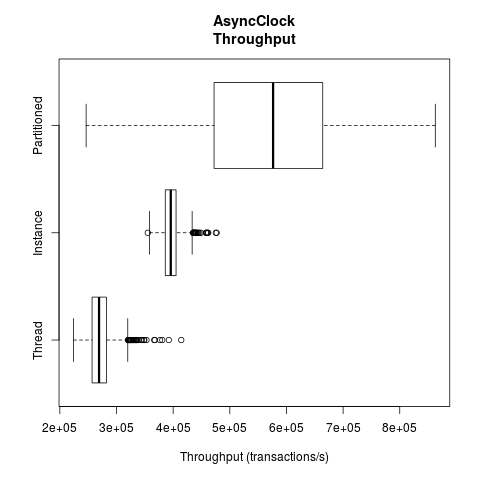
\includegraphics[width=.6\textheight]{async_throughput_box.png}
    \end{column}
  \end{columns}

  \vspace*{12pt}

  \fbox{
    \parbox{\linewidth}{
      \centering
      Instance/Partitioned are viable multi-threaded event schedulers!
    }
  }

\end{frame}

\begin{frame}{Scheduler Evaluation: SyncClock 
\includegraphics[height=12pt]{CLOCK01-300px.png}}

    \begin{columns}
    \begin{column}{.4\textwidth}
      \begin{itemize}
      \item Machine:  2 cores
      \item Instance/Partitioned:  2 threads
      \item Thread:  \emph{2 threads}
      \end{itemize}
    \end{column}
    \begin{column}{.6\textwidth}
      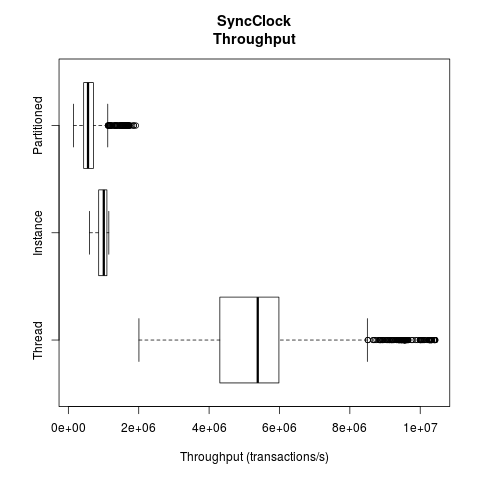
\includegraphics[width=.6\textheight]{sync_throughput_box.png}
    \end{column}
  \end{columns}

  \vspace*{12pt}

  \fbox{
    \parbox{\linewidth}{
      \centering
      Compilation beats interpretation!
    }
  }

\end{frame}

\begin{frame}{Conclusions and Future Work}
  \begin{block}{Conclusions}
    \begin{enumerate}
    \item Reactive component model enables principled composition/decomposition of reactive systems.
    \item Reactive component semantics can be checked efficiently.
    \item Empirical results suggest that reactive components could compete with optimized multi-threaded approaches.
    \end{enumerate}
  \end{block}

  \begin{block}{Future Work}
    \begin{itemize}
    \item Extend model for introduction and dynamic composition
    \item Explore additional scheduler classes and algorithms
    \end{itemize}
  \end{block}
\end{frame}

\begin{frame}
  \centering
  \Huge
  Questions?
\end{frame}

%% \begin{frame}
%%   \bibliographystyle{plain}
%%   \bibliography{slides}{}
%% \end{frame}

\begin{frame}
    \centering
  \Huge
  Bonus Slides
\end{frame}

\begin{frame}{Synchronized Two-Phase Calling Convention}

  \begin{columns}
    \begin{column}{.4\textwidth}
      To execute a transaction:
      \begin{enumerate}
      \item Depth-first traversal of transaction graph (immutable phase)
      \item Execute continuation of activate statements (mutable phase)
      \end{enumerate}
      \vspace*{12pt}
      \emph{Maps well to existing architectures!}
    \end{column}
    \begin{column}{.6\textwidth}
  \resizebox{!}{.7\textheight}{%
\begin{tikzpicture}
%% component boundary

\draw (0,-5) -- (0,7);
\draw (5,-5) -- (5,7);

\node at (2.5, 6.5) { ... };
\draw (0,6) -- (5,6);
\node at (2.5, 5.5) { argument (component pointer) };
\draw (0,5) -- (5,5);
\node (pip1) at (2.5, 4.5) { previous instruction pointer };
\draw (0,4) -- (5,4);
\node (pbp1) at (2.5, 3.5) { previous base pointer };
\draw (0,3) -- (5,3);
\node at (2.5, 2.5) { locals };
\draw (0,2) -- (5,2);
\node at (2.5, 1.5) { arguments to push port };
\draw (0,1) -- (5,1);
\node at (2.5, .5) { argument (component pointer) };
\draw (0,0) -- (5,0);
\node at (2.5, -.5) { arguments to push port };
\draw (0,-1) -- (5,-1);
\node (pip2) at (2.5, -1.5) { previous instruction pointer };
\draw (0,-2) -- (5,-2);
\node (pbp2) at (2.5, -2.5) { previous base pointer };
\draw (0,-3) -- (5,-3);
\node at (2.5, -3.5) { locals };
\draw (0,-4) -- (5,-4);
\node at (2.5, -4.5) { ... };

\node[anchor=west] (as1) at (5.5, 4.5) { activate statement body };
\draw[->] (pip1) -- (as1);
\node[anchor=west] (as2) at (5.5, -1.5) { activate statement body };
\draw[->] (pip2) -- (as2);

\draw[->] (pbp2) -- ++(-3,0) -- ++(0,6) -- (pbp1);

\node[anchor=west] (nil) at (5.5, 3.5) { nil };
\draw[->] (pbp1) -- (nil);

\node[anchor=west] (head) at (5.5, -2.5) { $head$ };
\draw[->] (head) -- (pbp2);

\draw[decorate,decoration={brace}] (-1,2) -- (-1,6) node[anchor=east,midway] { action };

\draw[decorate,decoration={brace}] (-1,-4) -- (-1,1) node[anchor=east,midway] { reaction };

\end{tikzpicture}
}%
    \end{column}
  \end{columns}
\end{frame}

\begin{frame}{Heaps}
  \begin{block}{Problem}
    Move state from one component to another efficiently
  \end{block}

  \begin{block}{Challenge}
    Maintain isolation of components (encapsulation)
  \end{block}

\end{frame}

\begin{frame}[fragile]{Heaps:  Approach}

  \begin{columns}

    \begin{column}{.5\textwidth}
      \begin{itemize}
      \item Run-time maintains a stack of heaps
      \item Top heap services allocation requests
      \item \verb+change+ scoping rules enforce encapsulation
      \item encapsulation enables parallel garbage collection
      \end{itemize}
    \end{column}

    \begin{column}{.5\textwidth}
      \begin{tikzpicture}
        [element/.style={on chain, draw, rounded corners, text width=10em, text centered},
          every join/.style={->, thick, shorten >=1pt},
          start chain=going above,
          node distance=.3cm]
        \node[element,join] {component1 (action)};
        \node[element,join] {component2 (reaction)};
        \node[element,join,green] {heap2.1 (change)};
      \end{tikzpicture}
    \end{column}

  \end{columns}

  \vspace*{24pt}

  \begin{center}
    One level of indirection for move and merge

    \begin{tikzpicture}
      \node [rectangle, draw] (p2) at (0,0) {0x12345678};
      \node [rectangle, draw] (p3) at (0,-1) {0x56781234};
      \node at (0,1) {* heap W};
      \node [rectangle, draw,blue] (hl) at (4,0) {0x90ABCDEF};
      \node at (4,1) {heap link};
      \node [rectangle, draw] (heap) at (8,0) {heap object};
      \node at (8,1) {heap (W root)};
      \draw [->,thick] (p2) -- (hl);
      \draw [->,thick] (p3) -- (hl);
      \draw [->,thick] (hl) -- (heap);
      \draw [dashed] (6, -.5) -- (6, .5);
    \end{tikzpicture}
  \end{center}

  \onslide<2>
  \begin{tikzpicture}[overlay,remember picture]
    \pgftransformshift{\pgfpointanchor{current page}{center}}
    \draw[red, very thick] (-1.3,-3.15) -- (1.1,-3.15);
  \end{tikzpicture}

\end{frame}

%% \begin{frame}

%%   Heaps may form hierarchies

%%   \vspace*{12pt}

%%   \begin{tikzpicture}
%%     [heap/.style={draw, rounded corners}]
%%     \node[heap] {component}
%%     child {
%%       node [heap] {heap1}
%%     }
%%     child {
%%       node [heap] {heap2}
%%       child {
%%         node [heap] {heap3}
%%       }
%%       child {
%%         node [heap] {heap4}
%%       }
%%     }
%%     ;
%%   \end{tikzpicture}

%% \end{frame}

\begin{frame}[fragile]{I/O}
  \begin{block}{Problem}
    Interact with external systems (through operating system)
  \end{block}

  \begin{block}{Challenges}
    \begin{itemize}
      \item Maintain fairness
      \item Avoid accidental sharing of state
    \end{itemize}
  \end{block}

  \begin{block}{Approach}
    \begin{enumerate}
    \item Introduce \verb+FileDescriptor+ type.
    \item Wrap \verb+FileDescriptor+s in reactive components.
    \item Introduce \verb+readable+ and \verb+writable+ predicates.
    \item Introduce functions for manipulating \verb+FileDescriptor+s.  All operations are non-blocking to ensure fairness.
    \end{enumerate}
  \end{block}
\end{frame}

\begin{frame}{Example:  Simple Network Time Protocol (SNTP)}
  \resizebox{\textwidth}{!}{
\begin{tikzpicture}
\draw (2,7.5) rectangle (4,9);
\node[below] at (3,9) {Timer};
\node (alarma) [shape=rightout, draw, fill=white] at (4,8) {Alarm()};

\draw (1.5,6) rectangle (16.5,10);
\node[below] at (8.5,10) {Sntp};
\node (alarmb) [shape=leftin, draw, fill=white] at (5,8) {Alarm()};
\node (senda)  [shape=rightout, draw, fill=white] at (11,8) {Send(UdpMessage)};
\node (receivea) [shape=rightin, draw, fill=white] at (11,7) {Receive(UdpMessage)};

\draw (12,6.5) rectangle (16,9);
\node[below] at (14,9) {UdpParticipant};
\node (sendb) [shape=leftin, draw, fill=white] at (12,8) {Send(UdpMessage)};
\node (receiveb) [shape=leftout, draw, fill=white] at (12,7) {Receive(UdpMessage)};

\draw (alarma.east) -- (alarmb.west);
\draw (senda.east) -- (sendb.west);
\draw (receiveb.west) -- (receivea.east);

\end{tikzpicture}
}
\end{frame}

\begin{frame}[fragile]{Example:  UdpParticipant}
\begin{lstlisting}
type UdpParticipant component {
  fd FileDescriptor;
  outQueue Queue;
  inQueue Queue;
  Receive push (msg $foreign UdpMessage);
}

init (this *UdpParticipant) Init () {
  this.fd = udp_socket()
}
\end{lstlisting}


\onslide<2>
\begin{tikzpicture}[overlay,remember picture]
  \pgftransformshift{\pgfpointanchor{current page}{center}}
  \node[
    rectangle callout,
    draw=eclipseGreen,
    ultra thick,
    fill=white,
    decorate,
    callout absolute pointer={(-1,1.8)},
    font=\Large,
    text width=0.6\textwidth,
    align=center,
    anchor=center
  ] at (2.5,0) {wrap a \verb+FileDescriptor+};
\end{tikzpicture}

\onslide<3>
\begin{tikzpicture}[overlay,remember picture]
  \pgftransformshift{\pgfpointanchor{current page}{center}}
  \node[
    rectangle callout,
    draw=eclipseGreen,
    ultra thick,
    fill=white,
    decorate,
    callout absolute pointer={(-.1,-1.1)},
    font=\Large,
    text width=0.6\textwidth,
    align=center,
    anchor=center
  ] at (2.5,0) {initialize a \verb+FileDescriptor+};
\end{tikzpicture}

\end{frame}

\begin{frame}[fragile]{Example:  UdpParticipant}
\begin{lstlisting}
reaction (this $const * UdpParticipant)
Send (msg $foreign UdpMessage) {
  var m UdpMessage = msg.Copy ();
  activate {
    this.outQueue.Push (m);
  };
}

action (this $const * UdpParticipant)
_send (!this.outQueue.Empty () &&
       writable (this.fd)) {
  activate {
    var m UdpMessage = this.outQueue.Front ();
    sendto (this.fd, m.host, m.port, m.msg);
    this.outQueue.Pop ();
  }
}
\end{lstlisting}

\onslide<2>
\begin{tikzpicture}[overlay,remember picture]
  \pgftransformshift{\pgfpointanchor{current page}{center}}
  \node[
    rectangle callout,
    draw=eclipseGreen,
    ultra thick,
    fill=white,
    decorate,
    callout absolute pointer={(.25,-.75)},
    font=\Large,
    text width=0.6\textwidth,
    align=center,
    anchor=center
  ] at (2.5,.75) {check status in precondition};
\end{tikzpicture}

\onslide<3>
\begin{tikzpicture}[overlay,remember picture]
  \pgftransformshift{\pgfpointanchor{current page}{center}}
  \node[
    rectangle callout,
    draw=eclipseGreen,
    ultra thick,
    fill=white,
    decorate,
    callout absolute pointer={(-3.1,-2)},
    font=\Large,
    text width=0.6\textwidth,
    align=center,
    anchor=center
  ] at (2.5,.75) {expose operating system calls};
\end{tikzpicture}

\end{frame}

%% \begin{frame}[fragile]{Example:  UdpParticipant}
%% \begin{lstlisting}
%% action (this $const * UdpParticipant)
%% _pre_receive (readable (this.fd)) {
%%   activate {
%%     var buf [64]byte;
%%     var r int = read(this.fd, buf[:]);
%%     var m UdpMessage;
%%     m.msg = copy(buf[0:r]);
%%     this.inQueue.Push (m);
%%   }
%% }

%% action (this $const *UdpParticipant)
%% _receive (!this.inQueue.Empty ()) {
%%   activate Receive (this.inQueue.Front ()) {
%%     this.inQueue.Pop ();
%%   }
%% }
%% \end{lstlisting}
%% \end{frame}

%% \begin{frame}{\rcgo{}:  Reference Semantics}

%% \rcgo{} is a \emph{race-free} programming language

%% \resizebox{\textwidth}{!}{%
%% \begin{tikzpicture}
%% [
%%   >=stealth',
%%   punkt/.style={
%%     rectangle,
%%     rounded corners,
%%     draw=black, very thick,
%%     text width=6.5em,
%%     minimum height=2em,
%%     text centered
%%   },
%%   pil/.style={
%%     ->,
%%     thick,
%%     %%shorten <=2pt,
%%     %%shorten >=2pt,
%%   }
%% ]

%% %% stacks
%% \node[punkt] (stack1) at (0, 0) {Stack 1};
%% \node[punkt,below=4cm of stack1] (stack2) {Stack 2};
%% \node[below=1cm of stack2] (stackdots) {...};
%% \node[punkt,below=1cm of stackdots] (stacks) {Stack S};

%% %% components
%% \node[punkt,right=1cm of stack1] (component1) {Component 1};
%% \node[punkt,below=4cm of component1] (component2) {Component 2};
%% \node[below=1cm of component2] (componentdots) {...};
%% \node[punkt,below=1cm of componentdots] (componentc) {Component C};

%% %% heaps
%% \node[punkt, text width=4.5em,below=1cm of component1] (heap1) {Heap 1};
%% \node[punkt] (heap2) at ($(component1) + (6,3)$) {Transferable Heap 1};
%% \node[punkt, below=1cm of heap2] (heap3) {Transferable Heap 2};
%% \node[below=1cm of heap3] (heapdots) {...};
%% \node[punkt, below=1cm of heapdots] (heaph) {Transferable Heap H};

%% \node[punkt] (heap21) at ($(heaph) + (-2,-2)$) {Transferable Heap H.1};
%% \node[punkt] (heap22) at ($(heaph) + (2,-2)$) {Transferable Heap H.2};

%% \draw[pil,->] (stack1) -- (component1);
%% \draw[pil,->] (stack1) -- (component2.north west);
%% \draw[pil,->] (stack1) -- (heap1.north west);
%% \draw[pil,->] (stack1) -- (heap2.west);

%% \draw[pil,<->] (component1.south) -- (heap1.north);
%% \draw[pil,->] (component1.east) -- (heap2.west);
%% \draw[pil,->] (component1.east) -- (heap3.west);
%% \draw[pil,->] (heap1.east) -- (heaph.west);

%% \draw[pil,->] (heaph) -- (heap21.north);
%% \draw[pil,->] (heaph) -- (heap22.north);

%% \path[pil] (stack1.west) edge [loop above, out=-135, in=135, min distance=1.5cm] (stack1.west);
%% \path[pil] (stack2.west) edge [loop above, out=-135, in=135, min distance=1.5cm] (stack2.west);
%% \path[pil] (stacks.west) edge [loop above, out=-135, in=135, min distance=1.5cm] (stacks.west);

%% \path[pil] (component1.north) edge [loop above, out=135, in=45, min distance=1.5cm] (component1.north);
%% \path[pil] (component2.north) edge [loop above, out=135, in=45, min distance=1.5cm] (component2.north);
%% \path[pil] (componentc.north) edge [loop above, out=135, in=45, min distance=1.5cm] (componentc.north);

%% \path[pil] (heap1.south) edge [loop above, out=-45, in=-135, min distance=1.5cm] (heap1.south);
%% \path[pil] (heap2.east) edge [loop above, out=45, in=-45, min distance=1.5cm] (heap2.east);
%% \path[pil] (heap3.east) edge [loop above, out=45, in=-45, min distance=1.5cm] (heap3.east);
%% \path[pil] (heaph.east) edge [loop above, out=45, in=-45, min distance=1.5cm] (heaph.east);

%% \path[pil] (heap21.east) edge [loop above, out=45, in=-45, min distance=1.5cm] (heap21.east);
%% \path[pil] (heap22.east) edge [loop above, out=45, in=-45, min distance=1.5cm] (heap22.east);

%% \end{tikzpicture}
%% }

%% \end{frame}

%% \makeatletter
%% \pgfdeclareshape{clock}
%% {%
%%   % All anchors are taken from the 'circle' shape:
%%   \inheritsavedanchors[from={circle}]%
%%   \inheritanchor[from={circle}]{center}%
%%   \inheritanchor[from={circle}]{mid}%
%%   \inheritanchor[from={circle}]{base}%
%%   \inheritanchor[from={circle}]{north}%
%%   \inheritanchor[from={circle}]{south}%
%%   \inheritanchor[from={circle}]{west}%
%%   \inheritanchor[from={circle}]{east}%
%%   \inheritanchor[from={circle}]{mid west}%
%%   \inheritanchor[from={circle}]{mid east}%
%%   \inheritanchor[from={circle}]{base west}%
%%   \inheritanchor[from={circle}]{base east}%
%%   \inheritanchor[from={circle}]{north west}%
%%   \inheritanchor[from={circle}]{south west}%
%%   \inheritanchor[from={circle}]{north east}%
%%   \inheritanchor[from={circle}]{south east}%
%%   \inheritanchorborder[from={circle}]%
%%   %
%%   % Only the background path is different
%%   %
%%   \backgroundpath{%
%%     % First the existing 'circle' code:
%%     \pgfutil@tempdima=\radius%
%%     \pgfmathsetlength{\pgf@xb}{\pgfkeysvalueof{/pgf/outer xsep}}%
%%     \pgfmathsetlength{\pgf@yb}{\pgfkeysvalueof{/pgf/outer ysep}}%
%%     %% \ifdim\pgf@xb<\pgf@yb%
%%     %%   \advance\@tempdima by-\pgf@yb%
%%     %% \else%
%%     %%   \advance\@tempdima by-\pgf@xb%
%%     %% \fi%
%%     \pgfpathcircle{\centerpoint}{\@tempdima}%
%%     %
%%     % Now the | and -- lines:
%%     \pgfmoveto{\centerpoint}%
%%     \pgflineto{\pgfpointscale{.5}{\pgfpointadd{\centerpoint}{\pgfpoint{0pt}{\pgfutil@tempdima}}}}%
%%     \pgfmoveto{\centerpoint}%
%%     \pgflineto{\pgfpointscale{.5}{\pgfpointadd{\centerpoint}{\pgfpoint{\pgfutil@tempdima}{0pt}}}}%
%%   }%
%% }
%% \makeatother

%% \begin{frame}

%%   trends slide - IIOT

%%   DDS to introduce problems with state of the art

%%   Contributions

%%   model

%%   \begin{center}
%%     {\LARGE Synchronous Reactive Systems}
%%     \vspace*{12pt}

%%     \begin{tikzpicture}
%%       \node at (0,2) {0};
%%       \node at (1,2) {1};
%%       \node at (2,2) {2};
%%       \node at (3,2) {3};
%%       \node at (4,2) {4};
%%       \node at (5,2) {5};
%%       \node at (6,2) {6};

%%       \fill[red] (1,1.25) rectangle (3,1.75);
%%       \fill[red] (4,1.25) rectangle (5,1.75);
%%       \draw (0,1.25) rectangle (6,1.75);

%%       \fill[blue] (0,.25) rectangle (4,.75);
%%       \fill[blue] (5,.25) rectangle (6,.75);
%%       \draw (0,.25) rectangle (6,.75);

%%       \draw[fill] (-1.5,1) circle [radius=.5];
%%       \draw[white] (-1.5,1) -- (-1.5,1.5);
%%       \draw[white] (-1.5,1) -- (-1, 1);
%%       \draw (-1,1) -- (-.5,1);
%%       \draw (-.5,1) -- (-.5,1.5);
%%       \draw (-.5,1) -- (-.5,.5);
%%       \draw (-.5,1.5) -- (0, 1.5);
%%       \draw (-.5,.5) -- (0, .5);
%%     \end{tikzpicture}
%%   \end{center}

%%   \rule{\textwidth}{0.4pt}

%%   \begin{center}
%%     {\LARGE Asynchronous Reactive Programs}
%%     \vspace*{12pt}

%%     \begin{tikzpicture}
%%       \draw[fill] (-1,1.5) circle [radius=.25];
%%       \draw[white] (-1,1.5) -- (-1,1.75);
%%       \draw[white] (-1,1.5) -- (-.75, 1.5);

%%       \draw[fill] (-1,.5) circle [radius=.25];
%%       \draw[white] (-1,.5) -- (-1,.75);
%%       \draw[white] (-1,.5) -- (-.75, .5);

%%       \draw (-.75,1.5) -- (6, 1.5);
%%       \draw (-.75,.5) -- (6, .5);


%%       \draw[fill,red] (0,1.5) circle [radius=.1];
%%       \draw[fill,red] (1,1.5) circle [radius=.1];
%%       \draw[fill,red] (2,1.5) circle [radius=.1] node (a) {};
%%       %\draw[fill,red] (3,1.5) circle [radius=.1];
%%       \draw[fill,red] (4,1.5) circle [radius=.1];
%%       \draw[fill,red] (5,1.5) circle [radius=.1];
%%       \draw[fill,red] (6,1.5) circle [radius=.1];

%%       \draw[fill,blue] (0,.5) circle [radius=.1];
%%       \draw[fill,blue] (.5,.5) circle [radius=.1];
%%       \draw[fill,blue] (1,.5) circle [radius=.1];
%%       \draw[fill,blue] (2.5,.5) circle [radius=.1] node (b) {};
%%       \draw[fill,blue] (3.5,.5) circle [radius=.1];
%%       \draw[fill,blue] (4,.5) circle [radius=.1];
%%       \draw[fill,blue] (6,.5) circle [radius=.1];

%%       \draw[->,>=stealth'] (a) -- (b) {};

%%       \node[draw, shape=ellipse, minimum height=2cm, minimum width=1cm] (so) at (2.25,1) {};

%%       \node () at (2.25, -.5) {synchronization};
%%     \end{tikzpicture}
%%   \end{center}
%% \end{frame}

%% \begin{frame}
%%   \frametitle{Limitations of the State of the Art}

%%   show a picture of a DDS like application

%%   show deadlock

%%   highlight the burden placed on programmer
%%   \begin{enumerate}
%%   \item identify and protect shared state
%%   \item understand the call graph
%%   \end{enumerate}

%% \end{frame}

\end{document}
